%
% $Id: thesis.tex 3914 2009-06-18 12:55:36Z sliske $
%
% See styles/readme.txt for further details and explanations on
% the used classes. 
%
% BE REMINDED, THAT WE EXPECT THE DIPLOMA THESIS TO BE TWOSIDED!
%
% Usage of the 'bsvs-thesis', which is based on KOMA default class
% 'scrreprt'. Thus the options are completely identical to the ones
% described by the KOMA-Doc (KOMA-Doc, Ch.3.1).
\documentclass[
  % Most of the default options are initiated well. (KOMA-Doc,
  % Tab.3.2), but some can be improved :-)
  % Additionally, KOMA offers some more options for its document
  % classes.
  %
  % Hint (LaTeX-Book Ch.2.1.1, Ch.A.5.4, Ch.A.5.8): The class options
  % set in '\documentclass' are directly passed through the single
  % '\usepackage'. Packages that are included via '\RequirePackage'
  % and '\LoadClassWithOptions' will get the options too.
  % If one option stays unused, there will be a corresponding LaTeX
  % warning during compilation.
  %
  % Compatibility options (KOMA-Doc, Ch.3.1.1)  
  % there is no option set yet, that bases on KOMA-Doc, Ch.3.1.1
  % Page spread options (KOMA-Doc, Ch.3.1.2)
  BCOR11mm, % Binding correction (unrequired? -> comment out [default=0])
  DIV12, % Number of divisions for the page spread construction (unrequired? -> comment out [default=9])
  % Layout options (KOMA- Doc, Ch.3.1.3)
  twoside, % two sided (unrequired? -> comment out [default='oneside'])
  headsepline, % separate head-line from content optically (horizontal row) (KOMA-Doc, Ch.'Kopf- und Fusszeilen')
  % Font family options (KOMA-Doc, Ch.3.1.4)
  % there is no option set yet, that bases on KOMA-Doc, Ch.3.1.4
  % List of content options (KOMA-Doc, Ch.3.1.5)
  liststotoc, % include list of tables/figures to list of content
  bibtotoc, % include list of literature to list of content
  idxtotoc, % include index to list of content
  % Lists of float environment options (KOMA-Doc, Ch.3.1.6)
  % there is no option set yet, that bases on KOMA-Doc, Ch.3.1.6
  % Formating options (KOMA-Doc, Ch.3.1.7)
  abstracton, % Put an coresponding header to the abstract (unrequired? -> comment out [default='abstractoff'])
  pointlessnumbers, % suppress ending dot in numberations (required? -> 'pointednumbers')
  %semidraft, % print 'draft' information, e.g. black border indicating oversized lines, DRAFT-watermark (unrequired? -> comment out [default='final'])
  % Now, there are other, KOMA-independend options that will be
  % provided to the required packages.
  %german % german modification of several LaTeX behaviour (unrequired? -> comment out)
]{bsvs-thesis}
\newenvironment{dtZusammenfassung}{\chapter*{\centering \normalsize Deutsche Zusammenfassung}}

% include thesis' meta data
\InputIfFileExists{thesis.cfg}{}{\ClassError{thesis.tex}{Missing file [thesis.cfg]!}{Create a configuration file.}}

\hyphenation{
   Soft-ware
   ad-ded
   compi-lers
}     
% 
% THE MAIN DOCUMENT
%

\begin{document}
\ofoot[\pagemark]{\pagemark}

% include intro
%
% $Id: intro.tex 2661 2008-06-05 13:54:42Z sliske $
%

% start with non paging
% note: authorship itself has another empty
\pagestyle{empty}
\cleardoubleemptypage
% title (includes acknowledgment/dedication)
\maketitle

% authorship
\cleardoubleemptypage

\makeauthorship

% abstract
\makeabstract
\cleardoubleemptypage
 
\makezusammenfassung
% table of contents
\cleardoubleemptypage
\pagenumbering{roman}
\pagestyle{plain}
\tableofcontents

\captionsetup[table]{skip=10pt}
% prepare main document
\cleardoublepage
\pagenumbering{arabic}
\pagestyle{chapterstyle}

% reset acronym counter
\acresetall
% include a chapter
%
% $Id: chapter1.tex 2908 2008-11-19 13:56:30Z sliske $
%

\chapter{Introduction}
\label{sec:intro}

Since the advent of the Internet, bandwiths available to both
commercial and private users have been ever increasing. While this opens up new possibilitys for high bandwiths
network applications, it also poses new security challenges for dealing with potentially malicious network traffic. In addition to traditional firewalls, 
\ac{HIDS} are a commonly used security measure, to protect a system  . Traditionally, \ac{HIDS} make use of application logfiles, which are parsed
for information on possible attacks and to identify malicious clients. The \ac{IPS} Fail2ban\cite{fail2ban} is 
is an one of the most prim
\par
The goal of this thesis will be the design and implementation of a new \ac{IPC} architecture for the
transmission of log messages, that is able to facilitate low latency communication
between sender and receiver. Additionally, the design should be able to scale to multiple
recipients, in order to accommodate more complex security system, in which several processes
require access to a hosts application log. For this purpose, a Proof of Concept \ac{IPS} will be 
developed, that utilizes the proposed \ac{IPC} architecture to receive log messages and ban malicious
clients in the style of Fail2ban. 


This thesis will be structured as follows: The following section provides background 
information on relevant concepts,  
% reset acronym counter
%%acresetall
% include a chapter
%
% $Id: chapter2.tex 2612 2008-06-03 18:32:54Z jozinke $
%

\chapter{Background} \label{sec:background}

The following section introduces the concept of \ac{HIDS} with the specific example of Fail2ban and presents the problem setting 
this thesis aims to solve. In addition to that, a short overview over common types of inter process communication and existing \ac{IPC} based logging solution is given. 
Finally, external libraries and other software used for the implementation and evaluation of the proof of concept \ac{IPS} are introduced.    

\section{Host-based Intrusion Detection / Prevention} \label{sec:hids}

Intrusion Detection Systems are tasked with monitoring and collecting data from target systems, which is then further processed and analyzed, to identify 
potential threads and facilitate a response \cite{vigna2006}.
The idea of specialized software for detecting intrusion attempts and other 
security threads goes as far back as 1980, when James Anderson published a study on 
``Computer security threat monitoring and surveillance'', which suggested the use of automated tools to assist with security monitoring\cite{anderson1980}. In 1987, Dorothy
Denning presented a seminal model for Intrusion Detection Systems, that proposed the use of pattern matching, based on
statistical analysis of audit records generated by a system, in order to detect abnormal user behavior \cite{denning1987}. 
Intrusion Detection Systems in general, can collect data from a multitude of sources. This allows for the distinction between \acp{NIDS} and Host-based Introduction Detection Systems (\ac{HIDS}). \ac{NIDS}
monitor network interfaces and analyze captured traffic, while \ac{HIDS} gather information directly provided by the hosts under their supervision. For the latter, this includes event logs of applications, as well as \ac{OS} based information,
such as user logins, file system operations or systemcalls. For analysis of the accumulated data, there a two commonly deployed strategies: 1. Misuse based detection relies on predefined 
patterns of misuse or malicious behavior, which are then matched against the observed data. 2. Anomaly based detection uses statistical analysis, to identify significant deviations
from normally observed behavior, which, in principal, enables the detection of attack patterns, that have not been previously observed. \cite{vigna2006} 

\subsection{Fail2ban} \label{sec:fail2ban}

Fail2ban is a open source Intrusion Prevention System \ac{IPS}, that is widely used to protect hosts against a range of network-based attacks, such as, for instance, brute-force login attempts \cite{fail2ban}. Intrusion prevention system constitute
a special class of \ac{IDS}, that not only detect an intrusion attempt, but also initiate an active response, with the aim of preventing or mitigating the attack. To identify potentially malicious clients,
Fail2ban uses a misuse detection approach, based on application logs. For configured applications, Fail2ban actively monitors their log and parses new entries based on a predefined filter. Fail2ban uses configuration units called `jails'  
, that allow for the customization to different applications. A jail defines a path to an application log, the filter being applied to the log messages within the logfile and an action, that
is executed on client matching the filter criteria. In addition to that, jails contain further parameters, such as the threshold of matches per client for the action to be executed,
as well as the duration of the action. The filter component of a jail defines a set of regular expressions, that are used to identify certain events in a log, like an unsuccessful login attempt or the 
exceeding of a request rate limit. The filter also obtains a clients IP address, to identify the client and datetime information, to determine, if the event occurred within a relevant time frame. 
Most commonly, the action issued by Fail2ban, is to ban the clients IP address. Fail2ban facilitates this via an \texttt{iptables} entry. 
\texttt{Iptables} is a utility program for Linux systems, that allows the interaction with the \texttt{netfilter} kernel framework, to implement packet filtering rules \cite{netfiler,iptables}. When banning a client, Fail2ban adds an iptables rule for the clients IP address, that leads 
to the dropping of all subsequent network packets from that address.
\par
Fail2bans netfilter-based approach of packet filtering has the disadvantage, of scaling poorly for large traffic rates, since packets need to traverse several processing steps of the kernel network stack, before they are ultimately discarded.
In his master thesis, Florian Mikolajczak proposed the alternative usage of eBPF programs, as a more efficient way of implementing packet filtering for intrusion prevention systems \cite{mikolajczak2022}. The \ac{eBPF}      
is an interface of the Linux kernel, that allows the event based execution of verified, user defined programs within the kernel. Packet filtering through \ac{eBPF} can be facilitated with an \ac{eBPF} program,
that is executed on incoming packets and delivers a verdict, of wether the packets should be dropped or further processed by the kernel. Via the \ac{XDP}, \ac{eBPF} programs can be attached to different hooks in 
the packet processing pipeline. For supported devices, programs can be attached in \texttt{XDP\_DRIVER} mode, where they are executed as part of the network device diver routine, very early into the packet processing. Florian Mikolajczak adapted an existing \ac{eBPF} program by Jesper Brouer
and Andy Gospodarek, to handle \ac{IPv6} traffic. He then integrated it with Fail2ban, to replace netfilter-based packet filtering. While he was able to demonstrate substantial performance improvements over netfilter-based filtering, his measurements 
revealed, that Fail2ban has significant performance issues, when faced with a large influx of log messages. 

\begin{figure}[h!]
	\centering
	\scriptsize
    \centerline{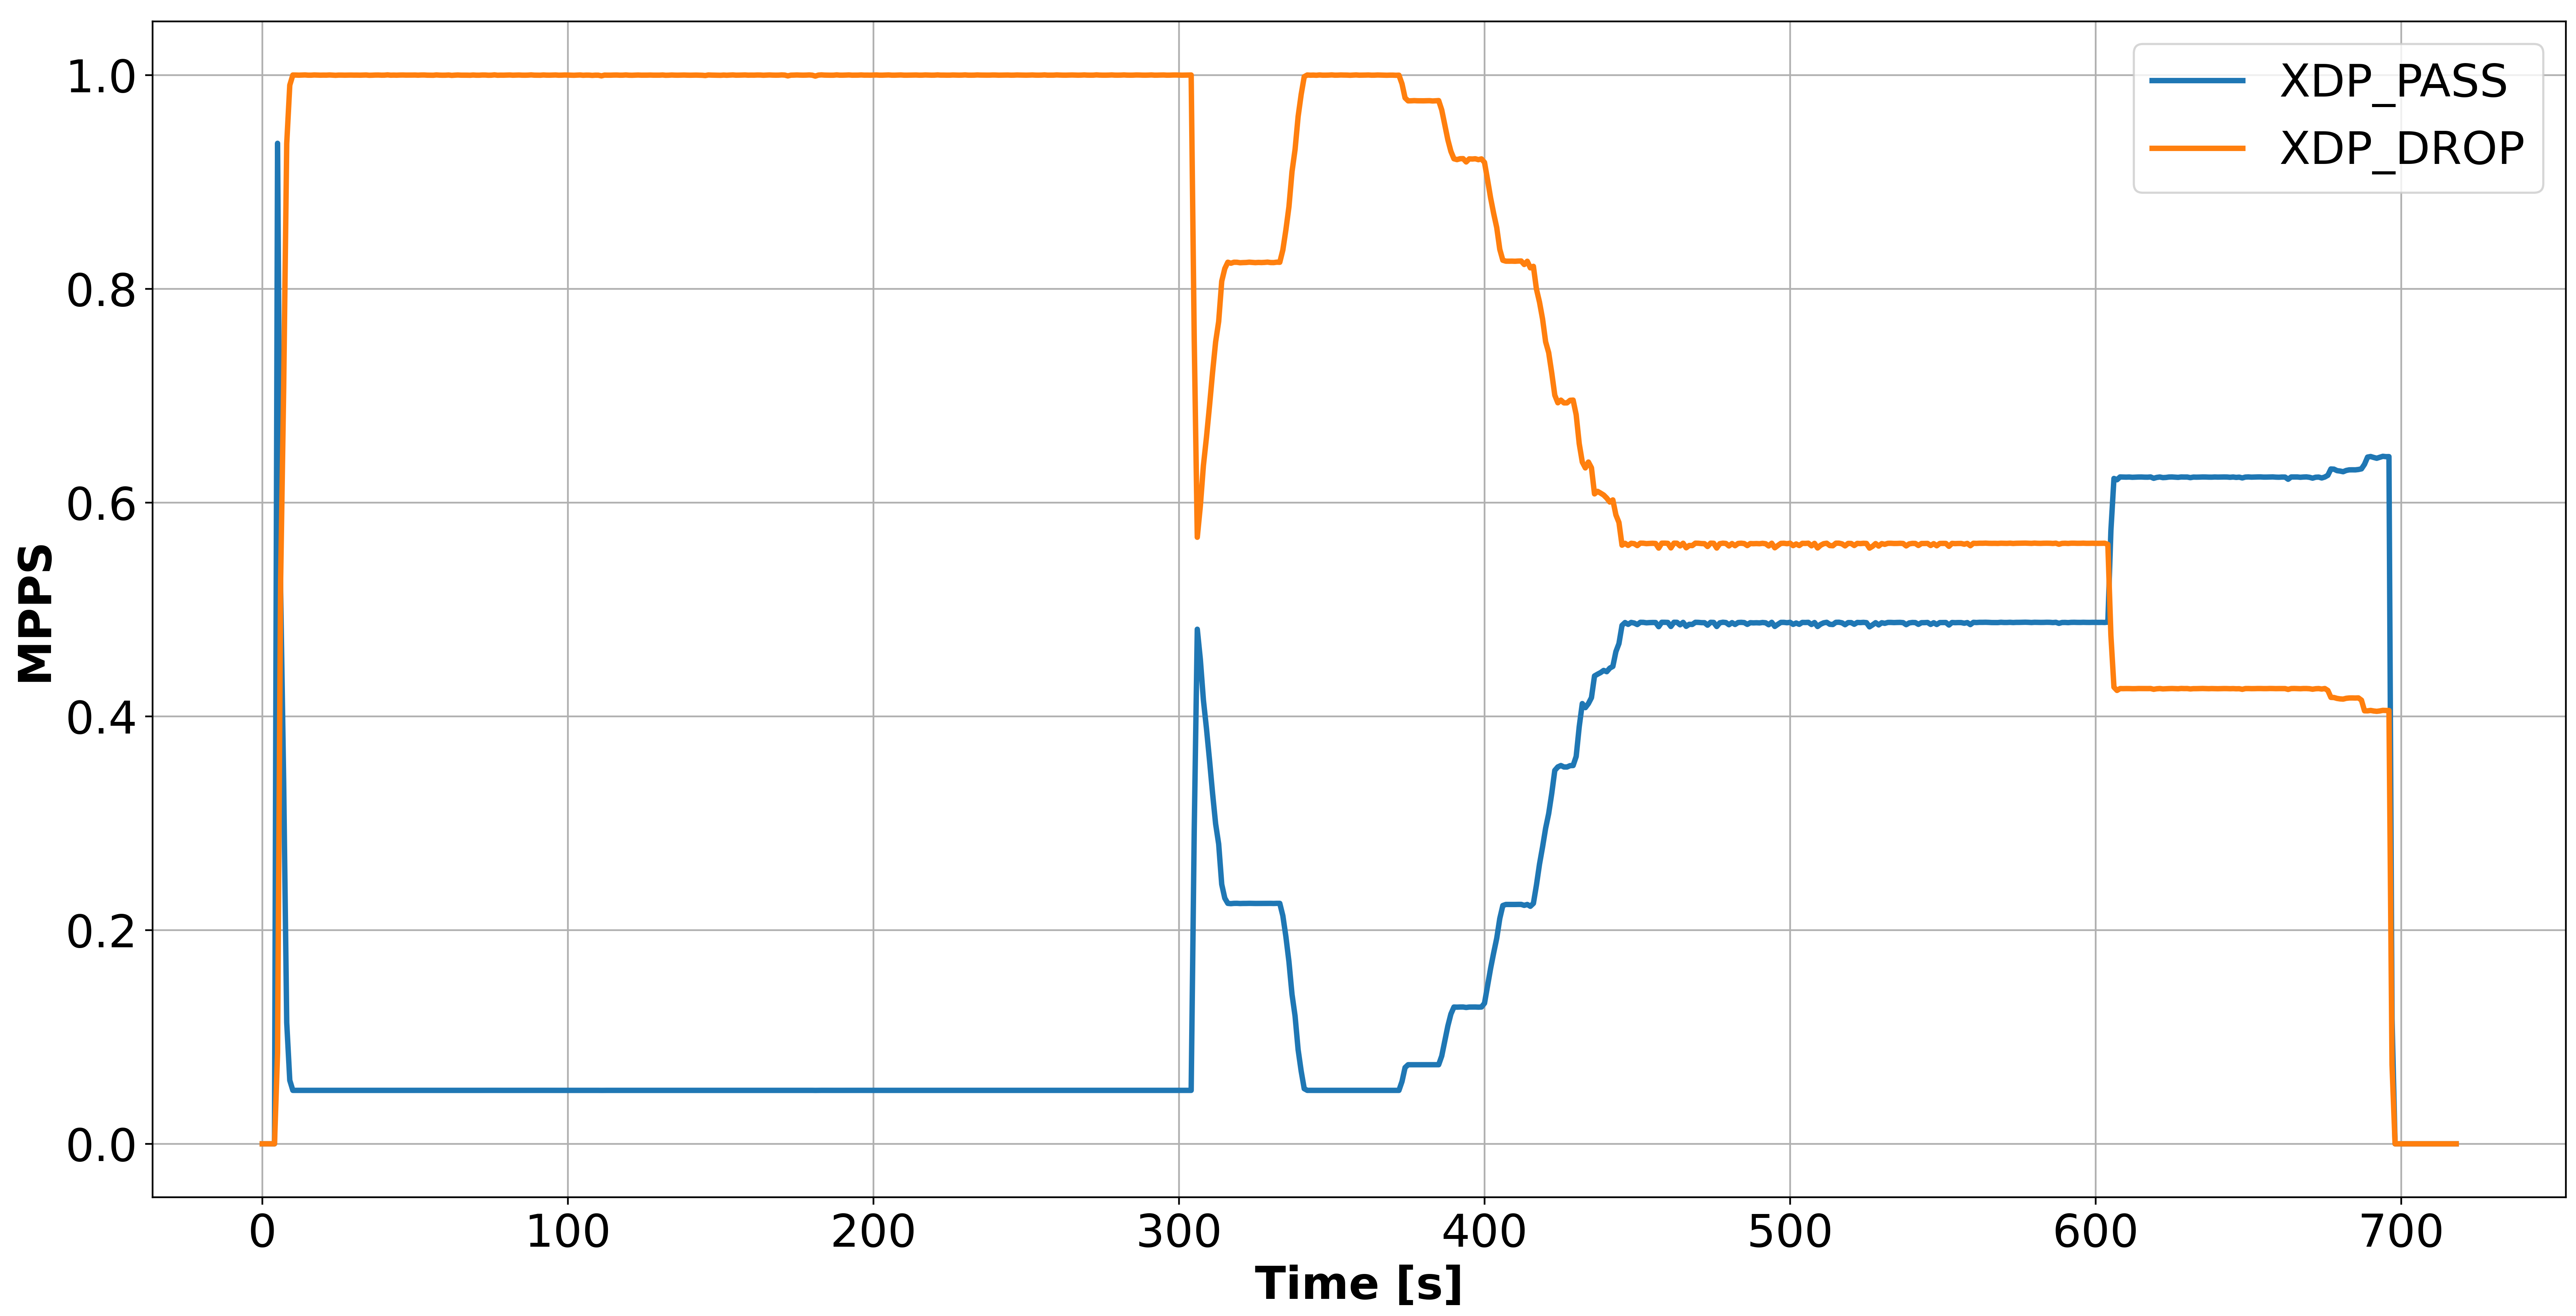
\includegraphics[width=1.2\textwidth]{images/Fail2Ban2.png}}
    \caption[Fail2ban measurement by \cite{mikolajczak2022}]{Results of experiment 1 from the  master thesis of Florian Mikolajczak \cite{mikolajczak2022}. In the experiment, 1 million \ac{PPS} of invalid traffic and 50 thousand \ac{PPS} of valid traffic where send to a server writing corresponding log messages for invalid requests. Fail2ban was 
	configured to ban clients for a duration of 300 seconds. Even in conjunction with more efficient \ac{eBPF} filtering, Fail2ban performed poorly, likely due to the slow speed of file-based log message transmission.}
	\label{fig:fail2ban:mikolajczak2022}
\end{figure}

Figure \ref{fig:fail2ban:mikolajczak2022} shows the results of the Fail2ban measurement conducted by Florian Mikolajczak. In the experiment, a BIND DNS Server received unwanted requests at a rate of 1 million \ac{PPS} from 254 different clients,
which resulted in corresponding entries in the servers rate-limit log. Fail2ban was configured to ban clients with rate limit violations for 300 seconds. Initially, the performance was as expected. However, after 
the end of the first ban cycle, Fail2ban failed to renew the ban for some clients, leading to a significant amount of unwanted traffic still reaching the application. Closer inspection of Fail2bans behavior indicated,
that the performance issues are likely the result of slow logfile parsing. Fail2bans rate of processing log entries appeared to be exceeded by rate of new entries, leading to Fail2ban falling increasingly further behind
in the processing of logged events. This constitutes a problem, as it essentially makes Fail2ban and by extension the protected host, vulnerable to \ac{DoS} attacks. This problem setting provides the primary motivation for this
thesis and will serve as a benchmark for the \ac{IPC} architecture and \ac{PoC} \ac{IPS} being developed. 

\section{Inter-Process Communication}
\label{sec:ipc}

\subsection{Types of IPC}
\label{sec:ipc_types}

Inter-process communication allows the exchange of data between different processes, through \acp{API} provided by the operating system. Since the development environment for this thesis will be Linux, the focus is restricted to \ac{IPC} APIs, that are available on UNIX-like systems.
\minisec{Shared Memory}
A commonly used mechanism, for sharing large amounts of data between two processes on the same system, is shared memory \cite[p.301ff.]{stevens1998ipc}.
Shared memory allows the allocation of a memory segment in \ac{RAM}, that can mapped into the address space of several processes. The memory segment has associated file permissions, 
allowing the creating process, to control the read and write access of other processes. Linux provides two main ways of creating
shared memory in the System V shared memory \ac{API} and the newer POSIX shared memory \ac{API} \cite{posixshm,systemvshm}. Processes can essentially treat shared memory like 
any other valid memory in their address space, which allows for fast and flexible application. A disadvantage of shared memory, at least for the aforementioned APIs, is its restriction 
to the local system boundaries, though solutions for network-based remote direct memory access exist \cite{recio2007}.
\par 
\minisec{Named Pipes / FIFOs}
Pipes, specifically named pipes, are a way of facilitating unidirectional data transfer between processes on a UNIX system. Named pipes have specific read and write file descriptors and are  
associated with a special file in the filesystem, which can be accessed by different processes. Pipes can be written to and read from via standard write and read system calls. The data is transmitted in 
a \ac{FIFO} manner, hence why named pipes are also commonly referred to as FIFOs. The maximum capacity, up to which a pipe can buffer data is limited, which by default is 65535 bytes on Linux, but can be adapted by a user. \cite{pipe}   
\par
\minisec{Sockets}
Sockets are another common \ac{IPC} type for data transfer, that allow for one-to-one as well as one-to-many 
communication, via a range of protocols\cite[p.57ff.]{stevens1998sock}. Sockets send data in formatted packets, that can be transmitted on a local host or via a network. For communication on a local system, UNIX systems offer UNIX Domain sockets. UNIX Domain sockets can be bound to a valid path in the filesystem, which serves as a way of addressing
the socket from another processes \cite{unixsock}. For data transfer beyond the local system, the Internet protocol \ac{IP} in conjunction with the \ac{TCP} or \ac{UDP} is most common. TCP offers connection oriented data transmission, that requires an orderly connection establishment, through a handshake between the commutating parties. It further ensures a reliable transfer of data, by       
detecting transmission errors trough acknowledgment and retransmitting unacknowledged packets. \ac{UDP} in contrast, provides no guarantees on reliable transfer, with the benefit of lower latency and less communication overhead. \cite[p.29ff.]{stevens1998sock}
\par
\minisec{Message Queues}
Finally, message queues are another commonly used \ac{IPC} mechanism, that allow the exchange of messages between processes. Linux natively supports the System V and POSIX message queue APIs, but third party
implementations exist as well, for instance the ZeroMQ library \cite{systemvshm,posixmsq,zeromq}. Message queues essentially function as a buffer, which can store messages up to a certain capacity. A writing process adds messages to the queue, while
reading processes remove messages from the queue. Unlike with sockets, writing and reading can occur asynchronously i.e. messages do not have to be read immediately after being added to a queue. ZeroMQ specifically, supports a range of common communication 
patterns. Among them are the publish-subscribe pattern, where a writer sends messages to multiple subscribed readers, or the request-reply pattern, that can be used, to implement remote procedure calls.         

\subsection{IPC based logging} \label{sec:ipc_logging}
Other than traditional file-based logging, syslog is a commonly used protocol to facilitate network based-logging
on UNIX-based systems. The syslog protocol was first developed in the 1980s by Eric Allman, as a solution
for centralized logging, and ultimately standardized by RFC 5424 \cite{gerhards2009}. Syslog operates on a server-client
basis, where logging clients send messages to a syslog server, that can be located on the host or a remote machine. This allows for
the aggregation of log events from different sources and also serves to functionally separate the generation of log messages from storing, analyzing
and further processing. 
Syslog messages have a standardized format, that contains sender information, date and time of the event, as well as a facility and severity code. The facility indicates
the category of the logging application, while the severity indicates urgency and impact of the logged event\footnote{A full list of codes can be found in \cite[p.10-11]{gerhards2009}}. 
The syslog protocol is most commonly used with \ac{UDP}, but does not specify a transport protocol and can also be used in 
encrypted form, via the \ac{TLS} protocol. 
Rsyslog is a modern implementation and extension of the syslog protocol, developed by Rainer Gebhards\cite{rsyslog}.
It is intended as a high-performance log processing system for enterprise systems, that allows the aggregation of log events
from a variety of sources, such as files, named pipes, sockets or message queues, via the \ac{AMQP}\cite{vinoski2006advanced}. 
\par
Logstash is another commonly used system, that supports \ac{IPC} based data aggregation \cite{logstash}. It provides input 
plugins for a range of inputs, including files, sockets, pipes and messages queues. Logstash is part of the Elasticsearch technology stack, that allows 
aggregation, processing and analysis of various data sources. Log aggregators, like Rsyslog and Logstash, have application in a security context,
as they can be integrated as part of \ac{SIEM} systems. \ac{SIEM} systems collect data from various security relevant contexts, such as firewalls or intrusion detection 
systems, to provide comprehensive real-time security monitoring and analysis of complex systems \cite{bhatt2014operational}.
\par
Regarding other high performance logging systems, the literature is, to the best of my knowledge, rather slim.
Jeong et al. present a shared memory based logging system for embedded UNIX-based applications \cite{jeong2013high}.
They use a memory mapped file, to buffer log messages between the logging application and a daemon processes, that is used for further forwarding of the messages.
Their logging systems achieves a more than 10 times larger message throughput and more than 100 times lower latency than traditional syslog, which they attribute 
to the pure use of user-level \ac{IPC} ,that avoids costly context switches to the kernel. 


\section{External Software} \label{sec:software}

\subsection{Hyperscan} \label{sec:hyperscan}
 
Hyperscan is a open source regular expressions matching engine developed by Intel. 
It is specifically designed for high performance use cases, such as the application in security contexts and is being used by the intrusion detection systems Snort and Suricata.  
The process of regular expressions matching with Hyperscan, is separated into compile- and run-time. At compile-time, a regular expressions in string representation are compiled into a 
database, with additional configuration options. These include the processing mode, which 
can be streaming, block or vectored mode. Streaming mode allows the scanning of a continuous data stream,
which is facilitated via a state, maintained between function calls. Block and vectored mode operate on data
that is readily available and can be scanned in a single call. Other compile options include 
case-less and multiline scanning, instructing Hyperscan to only match an expression
once, or to report the leftmost start index of a match\footnote{By default, only the end index of a match is provided.}. The latter, comes with detrimental performance implications.
Hyperscan allows the compilation
of multiple patterns into a single database, which can be scanned for in parallel. 
For scanning, Hyperscan allows the user to define a callback function, that is 
called when a match occurs. The matched pattern can be identified with an id parameter. \cite{hyperscan}
\par 
For the purpose of this thesis, Hyperscan will be used as the regular expression engine, for
the matching of patterns against log messages, received by the proof of concept \ac{IPS}.    

\subsection{io\_uring} \label{sec:io_uring}

io\_uring is an asynchronous \ac{IO} framework of the Linux kernel, that was first introduced in kernel version 5.1 \cite{io_uring}.
In contrast to traditional read and write systemcalls, io\_uring provides non-blocking \ac{IO} operations on
file descriptors. This is facilitated via in-memory queues, that are shared between a user process and the kernel.
The first queue is a submission queue, that the application uses, to register \ac{IO} operations to the
kernel. The second queue is a completion queue, that the kernel fills with information on completed \ac{IO} requests.
An application can register several \ac{IO} operations, which are ultimately submitted to the kernel.
The application can then continue execution, while the \ac{IO} operation is asynchronously executed by the kernel.
Via the completion queue, the application can poll the status of the submitted operations
and receive information about their completion.        
\par
Liburing is a library written by Jens Axboe, that provides a high level interface to the io\_uring framework \cite{liburing}.
It allows the setup of a a io\_uring instance, which can be subsequently used to conduct \ac{IO} operations
on files, but also other types of file descriptors, such as sockets.
\par
For the purpose of this thesis, liburing will be used to implement asynchronous file reading and writing,
for both the proof concept \ac{IPS}, as well as auxiliary applications. 

\subsection{TRex} \label{sec:trex}

TRex is a traffic generating tool developed by Cisco System \cite{trex}. It supports the generation of both
stateless as well stateful traffic, for network up to application layer protocols. TRex is build with the Data Plane Development Kit framework,
that offers user space based packet acceleration, enabling TRex to reach traffic rates up to 200Gb/s, given appropriate hardware support. 
Traffic can be generated either via pcap files or Python scripts, that use the packet manipulation library scapy \cite{scapy}.
\par 
For the purpose of this thesis, TRex will be used, to conducted measurements and evaluate the proof of concept \ac{IPS}.
During initial measurements, its was discovered, that TRex struggles to maintain the advertised traffic rates for stateful traffic in certain scenarios.
More specifically, the absence of an acknowledgment packet to a \ac{TCP}-SYN packet sent by TRex, appears to inhibit performance.
Hence, measuring a \ac{DoS} scenario, as described in section \ref{sec:fail2ban}, is problematic for \ac{TCP} based traffic, as SYN packets from banned clients
emulated by TRex will not be answered by a server protected by Fail2ban or the proof of concept \ac{IPS}. For this reason, all measurements conducted in this
thesis will be \ac{UDP} based.


% reset acronym counter
%%acresetall
% include a chapter
%
% $Id: chapter3.tex 3915 2009-06-18 13:28:32Z sliske $
%
%%\pagestyle{scrheadings}
%%\ohead[]{}
%%\ihead[]{}
%%\chead[]{}
%%\ofoot[\pagemark]{\pagemark}
%%\ifoot[]{}
\chapter{Design \& Implementation}
\label{sec:design}

The following section introduces the design and implementation of the proposed \ac{IPC} architecture and the proof of concept \ac{IPS}, as well as auxiliary libraries and applications.
First, the requirements and overall purpose of the design are defined and translated into an abstract architecture. Subsequently, the implementation for a concrete \ac{IPC} type is presented.


\section{Requirements}

The primary goal of the new \ac{IPC} based logging architecture is the ability to handle high load scenarios, like the \ac{DoS} scenario discussed in section \ref{sec:fail2ban}.
This includes the basic functional requirement of offering an API that can be used to send data to and receive data from different processes. Beyond that,
the architecture should be usable in a realistic context. For this purpose, the following requirements should be satisfied, in order of importance.
\begin{itemize}
    \item \textbf{Low latency} \\
    As discussed in \ref{sec:fail2ban},  the primary issue of file based logging in the context of \ac{IPS} appears to be a lack of transmission speed. Hence,
    offering low latency data transfer is a critical aspect of the new architecture. In a \ac{DoS} scenario, the \ac{IPS} need to receive information
    about malicious clients as fast as possible, in order to take countermeasures that lower the load on the system. 
    \item \textbf{Low overhead} \\
    Another problem with file based logging is, that both read and write operations require systemcalls, which lead to costly context switches between application and kernel. Using traditional
    file I/O, read and write operations are blocking, meaning that a program can only resume, once the operation has concluded. In a high load scenario, where potentially
    millions of log messages are written per second, this can cause significant communication overhead for both reader and writer. It also looses critical execution time to waiting,
    which, on the side of the writing server, lowers the availability of the service and on the reading \ac{IPS} side, reduces responsiveness to the ongoing attack. The new architecture should there offer low overhead communication,
    ensuring that both writer and reader are not spending a majority of their execution time writing or receiving log messages.
    \item \textbf{High bandwidth} \\
    In conjunction with  low latency, high bandwidth is required to ensure a fast transfer of large amounts of data. When processing millions of log events per second, the architecture
    needs to be able to execute a single data transfer quickly, but also allow for a large amount of data to be transmitted at once, to avoid a bottleneck between writer and reader.
    \item \textbf{Reliability} \\
    While not the primary concern, the architecture should in principal be able to transfer log messages reliably, even under a high load. Hence, message loss or corruption 
    should be kept to a minimum. This is to ensure, that the \ac{IPS} or other reading application are aware of entirety of all logged events and no potentially security relevant event is missed. 
    \item \textbf{Scalability} \\
    An advantage of file based logging is, that logged events are stored persistently and also accessible to a multitude of applications. Log data generated by an application may be relevant in different
    contexts, such as intrusion prevention, \ac{SIEM} or other non-security related uses. Therefore, the architecture should be able to scale to multiple readers that can access the log data in parallel. 
    \item \textbf{Integrability / Portability} \\
    Finally, to be of use in a realistic context, it is required that the architecture is able to integrate with existing applications. Since the goal if this thesis is a proof of concept and not an 
    API ready for use in production, this will be a lower priority requirement. However, the design should at a minimum offer a well defined and easily usable API, that can be realistically integrated into a real application
    and potentially further developed beyond the scope of this thesis. As part of that, the design should be portable to different systems and ideally not rely on special hardware of software support, other than what
    is commonly present on most Linux systems. The architecture should also be flexible i.e. impose as little restrictions as possible on the user, in order to be adaptable to a wide range of use case scenarios.  

\end{itemize}

The architecture proposed on this thesis will likely not be able to satisfy all listed requirements to the fullest. Potential tradeoffs between requirements exists and will have to be considered in the following
design. Where tradeoffs are impossible to avoid, the architecture should ideally offer configuration option, that allows the user to decide, which requirements should be prioritized.       

\section{Abstract Architecture}

To further illustrate the purpose and requirements of the desired architecture, an abstract architecture is provided.
The goal is to provide a high-level design, that formalizes a set of functional requirement, but leaves enough
flexibility to be implemented with different \ac{IPC} solutions.  

\begin{figure}[h!]
    \label{fig:abstract_architecture}
    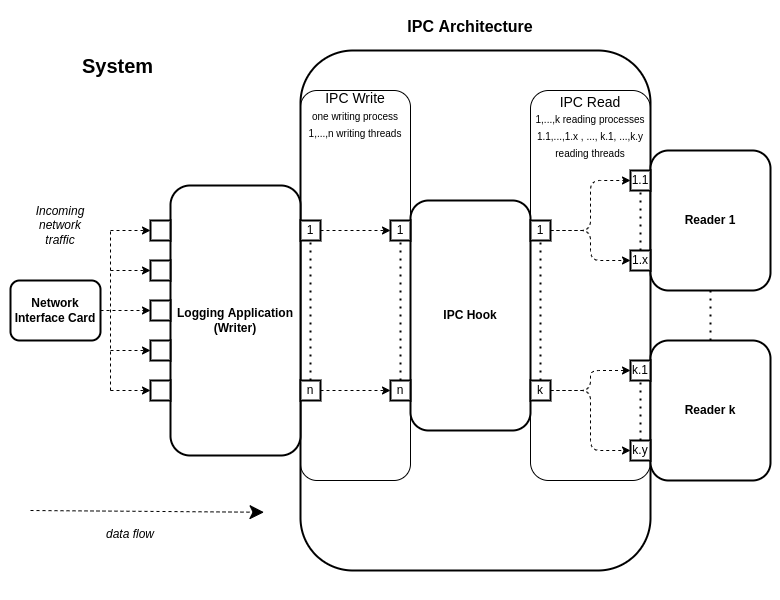
\includegraphics[width=\textwidth]{images/meta_ipc_architecture.png}
    \caption[IPC Architecture]{Abstract \ac{IPC} architecture }
\end{figure}

Figure \ref{fig:abstract_architecture} presents the abstract design for the proposed \ac{IPC} architecture.
The primary assumed use case is a producer consumer scenario, in which a single application writes log messages that 
are read by $k$ receiving processes. The transfer of data is assumed to be unidirectional, i.e. the roles of reader and writer are static for the duration of the
communication. An exception to this can be auxiliary messages for the setup, teardown or reconfiguration of the communication, that may require readers to send
data to the writer. The writer is assumed to be a server, that receives receives client request over a network.
On modern multi-core system, web servers like nginx and apache or a DNS server such as BIND usually use multiple threads to handle incoming request.
This allows for the parallel distribution of work onto the available CPU cores, making more efficient use of the systems resources. To efficiently accommodate a 
multi-threaded writer, the \ac{IPC} architecture is required to support a thread-safe write operation. Hence, it must be possible to
write in parallel from $n$ threads, without race conditions that could cause data corruption, or the need for additional thread synchronization    
on the writer side. On the reader side, the architecture must be able to support multiple reading processes, that each receive the entirety
of the written messages and are able to read in parallel. To allow load balancing on the reader side as well, the read operation
should also be capable of multi-threading. For the multi-threaded read within a reading process, the operation should enable a balanced an starvation-free distribution 
of messages to the calling threads.  
\par
Given the requirements and abstract architecture, the goal is to find a concrete implementation, that satisfied the proposed design.


\section{Choice of IPC Type}

During the development of this thesis, several \ac{ICP} mechanism where considered as suitable candidates for the proposed architecture. The initial
objectives was to create multiple implementation that each use a different \ac{IPC} type, in order to compare their performance empirically. 
To prevent the required time effort and scope of this thesis to get out of hand, the idea was abandoned in favor of a single implementation.
This has the additional benefit, of devoting more time to refine the concrete design and implement additional features. 
\par
All of the \ac{IPC} types introduced in section \ref{sec:ipc_types} 

\section{Ringbuffer API}

The following section presents the design and implementation of the shared memory based architecture for the transmission
of log messages. \\

\subsection{Design}
\label{sec:design}
For the base structure of the shared memory design, a ringbuffer was chosen. A ringbuffer is a queue-like data structure, used to store
multiple entries in a sequence. The entries are processed \ac{FIFO} manner, hence data is being read in the same order that is was written. 
Ringbuffers are a commonly used structure to buffer data streams, especially network application \cite{}.
They are usually realized as a fixed size array with additional pointers, that indicate the current location
of readers and writers within the buffer. When the end of the buffer is reached during a read or write operation, the pointer
wraps around to the begin of the buffer, threating the array, as if start and end where connected in a circular shape. 

\begin{figure}[h!]
    \label{fig:shm_architecture}
    \includegraphics[width=\textwidth]{images/shm_architecture.png}
    \caption[Shared Memory Architecture]{Architecture for the single-writer, multi-reader shared memory ringbuffer for the transmission
    of log messages. }
\end{figure}

Figure \ref{fig:shm_architecture} display the proposed ringbuffer architecture, adapted from the abstract design in Figure \ref{fig:abstract_architecture}.
The shared memory region consists of a global header as well as a variable amount of segments,
that each have their own segments header. Each segment constitutes a ringbuffer that is independent of the
the other segments. The global header contains contains information that is global to
the entire buffer and is used for initialization, when processes attach to the buffer. The buffer parameters within the global
header are initializes by the processes creating the buffer and are supposed to be constant for the lifetime of the shared memory segment.
The segment count variable indicates the amount of segments within the buffer. As illustrated
in \ref{fig:shm_architecture}, the number of segments is supposed to map 1:1 to the number 
of writing threads. Since each writing threads has their own ringbuffer, no synchronization for access
to the write pointers is required. The individual entries within the segment ringbuffers are fixed
size lines, the length of which in bytes is determined by the line size field in the global header. Each line corresponds
to one log message, the same way a line in a logfile would.  
Limiting buffer entries to a fixed maximum size has some obvious disadvantages. The primary concern
is inefficient use of memory, as the line size will have to be chosen to accommodate the largest possible log message, since multi line
messages are not intended in the design. If log messages vary greatly in length, this may cause a lot of unused memory
for shorter messages. The fixed size was chosen for a more convenient implementation of the overwrite feature, which is enable with the overwrite filed in the global header and will be covered in more detail
later. Allowing for variable length entries is still an important consideration for further development of the design. The line count variable in the global header 
determines the number of entries each segment ringbuffer has. Making all segments equal in size implicitly assumes, that the distribution of log messages written
is equal among the writing threads. However, variable size segments could be trivially added to the design, should a use case for that emerge. 
Finally, the global header contains a field for the number of allowed readers, as well as boolean fields, that indicate the attachment of the writer and the readers.
Keeping the number of allowed readers fixed limits the ability of dynamically adding new readers, but makes the implementation more convenient. The attachment field are used for
reference counting, of how many processes are attached to the buffer. When a reader attaches to the buffer, it will iterate through the readers attached array in the global header, in search of the first entry that that is not
set to true. If an entry is found, the reader will set the value of the entry to true and the index of the entry becomes the readers reader id. Since writing to the attachment fields 
is implemented via atomic compare exchange operations, no race conditions exist for simultaneously attaching readers. Similarly, the writer uses the write attached field when attaching to the buffer.
\par
Each segment of the buffer begins with its own header, that consist of a write index and an array of read indices, that is reader count elements long.
The index corresponds to a line in the segment and is used to keep track of the current position of the reader or writer in the buffer, as well
as to synchronize reader and writer. Both reader and write indices are implemented as atomic variables. Hence, read and write operation 
are executed like a single CPU instruction. This eliminates the possibility, that a processes can read the index of another processes while it is being written and
potentially obtain a corrupted value. Using atomic indices allows for lock free synchronization of reader and writer, which avoids the performance impact of having to
switch threads between waiting and execution states that result from lock-based synchronization. However, atomic operations are also more costly compared to regular reads writes \footnote{The performance evaluation of atomic vs lock based synchronization is not part of this thesis, but could be a consideration for a potential further development of this architecture.}. 
The lines of the segment begin below the segment header. The segment buffer capacity in bytes is given by line size "*" line count and the capacity of the entire buffer is given by segment capacity "*" segment count.  

\subsection{Implementation}
In the following, the implementation of the design in figure \ref{fig:shm_architecture} and relevant API functions is presented.
The entire API was implemented as a static library in C. The associated header and source files are \texttt{shm\_rbuf.h} and \texttt{shm\_rbuf.c}, which can be found 
under src/lib in the Git repository for this thesis \cite{gitlab}. All API functions return numeric error codes, the meaning of which is also documented in \texttt{shm\_rbuf.h}.  
\par
\begin{algorithm}[h!]
    \lstinputlisting[language=c, firstline=86, lastline=92]{listings/shm_ringbuf.h}
    \label{alg:shm:set_clean}
    \caption[Shared Memory Ringbuffer: Initialization and Cleanup]{Initialization and cleanup function for the shared memory ringbuffer.}
\end{algorithm}
Algorithm \ref{alg:shm:set_clean} displays the function signature for  the initialization and finalizations functions.
\texttt{shmrbuf\_init} is used to create or attach to an existing shared memory buffer and has to be called before read or write operations
on the buffer can be executed. \texttt{shmrbuf\_finalize} is the corresponding function to detach or destroy the shared memory buffer and should be called
upon ending the interaction with the buffer, for instance when exiting an application. \texttt{shmrbuf\_finalize} will only destroy the shared memory segment,
if no other process is attached. Otherwise the memory will simple be unmapped and the attachment field in the global header (as described in \ref{sec:design}) is released. 
\texttt{shmrbuf\_init} and \texttt{shmrbuf\_finalize} can be called by both reader and writer 
processes, which is why a role has to be specified as an additional parameter in the function call. The role determines, what type of struct the union pointer shmrbuf\_arg\_t is being cast to,
which contains further parameters used by the functions. 

\begin{algorithm}[h!]
    \lstinputlisting[language=c, firstline=27, lastline=36]{listings/shm_ringbuf.h}
    \label{alg:shm:writer_arg}
    \caption[Shared Memory Ringbuffer: Writer Parameters]{Structure to store writer parameters for the shared memory ringbuffer.}
\end{algorithm}

Algorithm \ref{alg:shm:writer_arg} displays the struct, that is used by a writing processes, to store and pass related parameters to the API functions.
In the current implementation, creation of a buffer can only be performed by a writing process. The reason for this is, that parameters such as the line
size of segment count need to be tailored to the writing process. The writer creates a new buffer by parameterising a \texttt{shmrbuf\_writer\_arg\_t} structure with
the desired parameters for the buffer and calling \texttt{shmrbuf\_init}. In addition to the already discussed parameters line size and line, segment and reader count, 
a key parameter is required. The key has to be a valid filepath within the file system and is used by System Vs shared memory API, to identify the shared segment\footnote{The System V shared memory API \cite{systemvshm} was used instead of the more modern POSIX API, since its support for memory allocation with huge pages was more convenient. Allocating the buffer with huge pages, should make read and write operations on a large buffer more efficient, since fewer entries are required in the translation lookaside buffer (TLB), making TLB misses less likely.}.  
If no shared memory segment referenced by the given path exists, a new segment of appropriate size will be allocated and mapped into the calling processes address space. Subsequently, its global header will 
be initialized with the parameters provided in the \texttt{shmrbuf\_writer\_arg\_t} structure.  

\begin{algorithm}[h!]
    \lstinputlisting[language=c, firstline=50, lastline=58]{listings/shm_ringbuf.h}
    \label{alg:shm:global_hdr}
    \caption[Shared Memory Ringbuffer: Global Header]{Structure to represent the global header of the shared memory ringbuffer.}
\end{algorithm}

Algorithm \ref{alg:shm:global_hdr} displays the structure for the global header of the shared memory buffer. When the header has been initialized
the checksum field is set to the sum over all constant header fields of the header. This is done as an additional security check for other processes attaching to the buffer. 
If the checksum is not correct, \texttt{shmrbuf\_init} will fail, to avoid writing to or reading from potentially corrupted memory. After initializing the header,
\texttt{shmrbuf\_init} sets the indices of all segment headers to zero. As an alternative to creating a new buffer,
a writer can also reattach to an existing buffer. When reattaching, the buffer parameters provided in \texttt{shmrbuf\_writer\_arg\_t} are ignored. To enable reattachment, the \texttt{REATT} flags has to be specified in the flags field of the shmrbuf\_writer\_arg\_t, otherwise the call   
to \texttt{shmrbuf\_init} will fail for an existing buffer. Reattachment is included in the API, so the writing application can be restarted (for instance for maintenance) without the need to
destroy the shared memory segment, if readers are attached. The overwrite feature is also specified via the flag field by specifying the \texttt{OVWR} flag.
Finally, \texttt{shmrbuf\_init} initializes an array of segment header structures in \texttt{shmrbuf\_writer\_arg\_t} and sets the \texttt{global\_hdr} pointer to point to the start of the shared memory segment.

\begin{algorithm}[h!]
    \lstinputlisting[language=c, firstline=67, lastline=71]{listings/shm_ringbuf.h}
    \label{alg:shm_seg_write}
    \caption[Shared Memory Ringbuffer: Writer Segment Header]{Structure to store writer information for a segment of the shared memory ringbuffer.}
\end{algorithm}
Algorithm \ref{alg:shm_seg_write} displays the structure  used in the segment header array. The structure does not represent the actual segment header the way its layed out in memory, but holds convenience pointers for a segment, that are used for writing operations.   
   
\par
For readers, attaching to an existing buffer is also done with a call to \texttt{shmrbuf\_init}. This functions analogous the writer, with the exception that the
shared memory segment pointed to by the provided path has to exist. 
\begin{algorithm}[h!]
    \lstinputlisting[language=c, firstline=38, lastline=46]{listings/shm_ringbuf.h}
    \label{alg:shm:reader_arg}
    \caption[Shared Memory Ringbuffer: Reader Parameters]{Structure to store reader parameters for the shared memory ringbuffer.}
\end{algorithm}
Algorithm \ref{alg:shm:reader} displays the structure used for storing reader parameters. If the attachment to the shared memory segment
and the checksum were successful, the reader will obtain a unique reader id, as described in section \ref{sec:design}. If all reader slots are already occupied, the \texttt{shmrbuf\_init} call fails.
Subsequently, \texttt{shmrbuf\_init} will initialize the pointers to the global header and the array of segment headers structures in the provided \texttt{shmrbuf\_reader\_arg\_t} structure.  
Readers have their own structure for storing segment header information, which is displayed in Algorithm \ref{alg:shm:seg_read}.  
\begin{algorithm}[h!]
    \lstinputlisting[language=c, firstline=60, lastline=65]{listings/shm_ringbuf.h}
    \label{alg:shm:seg_read}
    \caption[Shared Memory Ringbuffer: Reader Segment Header]{Structure to store reader information for a segment of the shared memory ringbuffer.}
\end{algorithm}

The structure includes a pointer to the index of the reader within the segment header. Which read index of a segment header is assigned to a reader, is determined 
by their reader id. Additionally, the structure contains a mutex lock, that is used to synchronize access to the segment when reding with multiple threads.
After a successful call to \texttt{shmrbuf\_init}, both reader an writer can start using their respective APIs for the buffer.

\subsection{Write API}

\begin{algorithm}[h!]
    \lstinputlisting[language=c, firstline=94, lastline=103]{listings/shm_ringbuf.h}
    \label{alg:shm:write_api}
    \caption[Shared Memory Ringbuffer: Write API]{Write API for the shared memory ringbuffer.}
\end{algorithm}

Algorithm \ref{alg:shm:write_api} displays the write API for the shared memory ringbuffer. \texttt{shmrbuf\_write}
writes a single log message to a specified segment within the buffer. The segment being written to has to be reference with an id, which is simply its index within $\{0..n\}$, where
n is the number of segments. The src argument is a pointer to the string that should be written to the buffer and \texttt{wsize} specifies the length of the string.
If \texttt{wsize} exceeds the line size specified in the global header of the buffer, the write operation will fail with a size error. When issuing a call to \texttt{shmrbuf\_write} without overwrite, the 
the function will atomically load all reader indices in the segment header and check their distance to the write index. If no reader is directly ahead of the write index, the line will be written
to the buffer and the writer index will be atomically updated to its new position, otherwise, the function call returns with an error. If the overwrite operation is specified in the header, synchronization between writer and reader is
effectively disabled and the write operation will conclude, regardless of the readers positions. This incurs the risk, that a reader and writer simultaneously access 
the same line, which may potentially corrupt the data being read. An advantage of overwrite is, that the writer avoids costly atomic operations and also cant be blocked 
by a slow or stale reader. The performance of the overwrite feature will be evaluated in section \ref{sec:evaluation}.
The write API provides a seconds write function in \texttt{shmrbuf\_writev}. Instead of writing a single line, the function receives an  
an array of \texttt{iovec} structures. The \texttt{iovec} structure defined in \texttt{struct\_iovec.h} within the standard C library, is a generic container for vectored
io operations. It contains a void pointer to a data field and a variable to specify the length of the data in bytes. 
shmrbuf\_writev works analogous to \texttt{shmrbuf\_write}, with the only difference that \texttt{vsize} lines referenced the corresponding \texttt{iovec}
structure in iovecs will be written to the buffer. Performance inspection of \texttt{shmrbuf\_write} with the benchmarking tool
perf \cite{perf} revealed, that about 75\% of the execution time is being spent for executing the atomic operations. Hence, 
using a vectored write operation should improve performance, as the synchronization only has to be applied once for multiple log messages.
For the sake of performance, neither write function implements synchronization for the write index. Calling a write operation
on the same segment from two different threads, is therefore not thread-safe.

\subsection{Read API}

Algorithm \ref{alg:shm:read_api} presents the functions of the reader API.
\begin{algorithm}[h!]
    \lstinputlisting[language=c, firstline=105, lastline=133]{listings/shm_ringbuf.h}
    \label{alg:shm:read_api}
    \caption[Shared Memory Ringbuffer: Read API]{Read API for the shared memory ringbuffer.}
\end{algorithm}

\texttt{shmrbuf\_read} is the corresponding read operation to \texttt{shmrbuf\_write}. It reads a single from
the specified segment into the provided buffer. If the provided buffer size is exceeded by the
size of the line, the read call fails, hence, the buffer should always at least have maximum line size, specified 
in the global header. Upon a call to \texttt{shmrbuf\_read}, the function atomically loads the write index for the segment. 
If the position of the write index differs from that of the readers read index, the line pointed to by 
the reader index will be copied to the external buffer and the read index will be atomically updated to its new position.
On success, \texttt{shmrbuf\_read} returns the (maximum) line size or zero, if the buffer is empty \footnote{In its current implementation, the buffer allows any type of binary data to be copied to a line. This is a problem for determining the actual length of a string
in the line buffer, since the terminating zero byte could still be part of the payload. Therefore, the maximum line length is always returned. Restricting the buffer to
non zero characters, or moving to a variable line length design, would enable the function to determine the length of the string contained in the line buffer, making the return value more meaningful.}.     
Analogous to the write API, a vectored read function exists in \texttt{shmrbuf\_readv}, which should incur the same performance benefits.
Instead of reading a single line, \texttt{vsize} lines are copied to the buffers specified by in corresponding \texttt{iovec} structures in \texttt{iovecs}.
Unlike the write API, all read operations called on the same segment by threads within the same processes are thread safe. 
At the beginning of each read operation, the mutex lock in the corresponding \texttt{shmrbuf\_seg\_rhdr\_t} structure is claimed and release after the read index has been updated.
For performance reasons, frequent locking of a segment by different reading threads should be avoided and threads should ideally be assigned segments that they access exclusively.
The read API contains to further functions. \texttt{shmrbuf\_read\_rng} is a convenience wrapper around \texttt{shmrbuf\_read}. It its useful for the case, that the reading
application uses fewer reading threads than there are segments in the buffer. shmrbuf\_read\_rng allow the specification a segment range through the upper
and lower parameters. When calling \texttt{shmrbuf\_read\_rng}, the function will iterate over all segments in the range in a round-robin fashion and perform a read call, until the first non empty segment is found or one cycle is completed.
The iteration index is persistent across function calls, ensuring that subsequent calls will continue the round-robin at the same position. This allows
starvation-free reading from the specified segment range. The boolean pointer \texttt{wsteal} allows for the option of workload stealing.
If \texttt{wsteal} is non null and all segments within the specified range are empty, the function will additionally iterate over all
segments outside of the specified range until a line has been read successfully or all segments have been checked. If a line was read from 
outside the specified range, \texttt{wsteal} will be set to true. The intention of the workload stealing feature is to mitigate scenarios,
where writing operation are not equally distributed across segments. If a reader, for instance, assigns two reading threads to one segments each,
but only one of the segments is being written to, then one reading thread would be idle, while the other has to handle all reading operations.
Workload stealing mitigates this, by having threads read across their assigned boundaries, if they would otherwise be idle.
\texttt{shmrbuf\_readv\_rng} is the last function in the read API and corresponds to \texttt{shmrbuf\_read\_rng} with the only difference,
that multiple lines can be read from each segment, up to the number specified by \texttt{vsize}. The \texttt{wsteal} parameter is
also an integer instead of a boolean pointer and will be set to the number of lines read from outside the specified range, if \texttt{wsteal} is non null.

\section{Proof-of-Concept IPS}

The following section presents the design and implementation of the proof of concept \ac{IPS}, for testing the \ac{IPC} architecture covered in the past sections.
In order to be comparable, the \ac{IPS} will be closely modelled after Fail2ban. The goal is however not to fully reimplement Fail2bans full set of feature, as that would go beyond
the scope of this thesis. Instead, a minimal set of features will be supported, the allows for the replication of the experiment covered in section \ref{sec:fail2ban}. 
The requirements for the \ac{Poc} are as follows:
\begin{itemize}
    \item Ability to monitor an application log, via traditional logfile parsing and the new \ac{IPC} solution.
    \item Ability to parse log messages with a customly definable regular expression.
    \item Ability to create filter rules for a clients IP addresses for both \ac{IPv4} \& \ac{IPv6}.
    \item Support for a ban limit, i.e. a customly definable number of matches per client before a ban is executed.
    \item Support for a ban time, i.e. a customly definable duration for the ban of a clients IP address. 
\end{itemize} 

Figure \ref{fig:ips_architecture} illustrates the proposed design for the \ac{PoC}, which will from hereon be referred to as Simplefail2ban. The source file 
for the implementation of Simplefail2ban is \texttt{simplefailban.c} in the \texttt{src/programs} directory of the thesis Git repository \cite{gitlab}.


\begin{figure}[p]
    \includegraphics[width=\textwidth]{images/ips_architecture.png}
    \caption[Simplefail2ban Architecture]{Activity diagram for the proof-of-concept IPS implementation. A variable number of ``banning threads'' receive log messages from a host and
    parse them with a predefined regular expressions. For messages that match the expression, the clients IP address is extracted from the log message and added to a hashtable, that keeps count of
    the number of matches per address. If the count reaches the configured limit, the address is added to the list of banned addresses with a current timestamp and inserted into the eBPF map. One ``unbanning
   thread'' routinely iterates through the banned list and checks, if a clients bantime hast elapsed. Clients with an elapsed bantime are removed from the eBPF map, banned list and hashtable.}
   \label{fig:ips_architecture}
\end{figure}

The functionality of the application will be separated into two classes of threads. A variable number of ``banning'' threads
and a single ``unbanning'' thread. The banning threads are tasked with monitoring the application log. The routinely call a read
function, to check if new messages have been added to the log. The read function varies, depending on the type of \ac{IPC} architecture
being used. For multi-threaded use, the read function has to be thread-safe and should ideally be lock free, to allow for optimal performance.
When using the shared memory ringbuffer as the source for log messages, \texttt{shmrbuf\_readv\_rng} is used, where the buffer segments
are equally distributed among the banning threads. For traditional logfile parsing, a custom read function was implemented, on the
basis of the asynchronous \ac{IO} library liburing introduced in \ref{sec:io_uring}.

\begin{algorithm}[h!]
    \lstinputlisting[language=c, firstline=27, lastline=35]{listings/uring_getline.h}
    \label{alg:uring_getline}
    \caption[Asynchronous Getline Function]{Function signatures for the io\_uring based getline functions.}
\end{algorithm}

\ref{alg:uring_getline} displays the function signatures. \texttt{uring\_getline} was modelled after the getline function
from the \texttt{stdio.h} library within the C standard library \cite{getline}. The function is passed a pointer to a \texttt{file\_io\_t} structure   
which contains file descriptor for the designated file, as well two buffers for the data being read. When the function is called, both buffers are checked for lines from an earlier function call.
If both buffers are empty, a liburing based read operation
is initiated. The read data is then tokenized into lines via a linear search for newline characters. If the read operation fills the entire buffer, another read
operation is scheduled for the second buffer. The return of the read operation is not awaited and will only be checked on a subsequent function call. The idea is,
that, in anticipation of subsequent function calls, data is being asynchronously read ahead, so that for most function calls, the function can resort to the buffer instead
of reading from the actual file. This should hopefully be more performant than regular blocking calls to \texttt{read}. The file offset for the read operation is tracked in
the \texttt{file\_io\_t} structure and updated after each read. \texttt{uring\_getlines} works analogous to \texttt{uring\_getline}, with the difference that up to \texttt{vsize}
lines can be read in a single function call. The lines and their size in byte are copied to the corresponding \texttt{iovec} structure in \texttt{iovecs}.
\texttt{uring\_getline} and \texttt{uring\_getlines} are not build for thread-safety, hence, the logfile based version of Simplefail2ban only supports single threaded monitoring\footnote{It its unclear, wether multi-threaded file reading would provide a performance benefit, since the read operations would have to be serialized by the operating system. Hence the decision to not support multi-threading.}.
\par
If a banning thread has successfully read one or multiple log messages, the messages are then matched against a regular expressions, which can be defined at the start of the application.
For \ac{Regex}-matching the regular expressions engine Hyperscan, introduced in section \ref{sec:hyperscan}, is used. Hyperscan is used in multi-pattern matching mode, scanning
for both the provided \ac{Regex} as well as expressions for \ac{IPv4} and \ac{IPv6}, to extract the clients \ac{IP} address from the log message. If the message was successfully matched against
the provided \ac{Regex}, the clients \ac{IP} address identified by the \ac{IP}-\ac{Regex} will be translated to its binary form for further processing. If the scan does not find a match, 
the processing moves on to the next log message. Alternatively, Simplefail2ban can also be configured to directly translate the entire log message to an \ac{IP} address, without regular expression matching.
This is not explicitly referenced in \ref{fig:ips_architecture} and was only implemented as reference, to measure the impact of \ac{Regex}-matching on the overall performance of the application.
\par
Once a clients binary \ac{IP} address has been determined (either through successful matching or direct translation), a hash table lookup for the address is performed.
The purpose if this is to determine, if a client has reached the ban limit, which is configured at the start of the application. 
The hash table stores key value pairs, where the key can be a \ac{IPv4} or \ac{IPv6} address in binary form and the value is a counter,
indicating the number of times the key has been queried. A custom hash table was implemented as a static library, the sources files for which are \texttt{ip\_hashtable.h}
and \texttt{ip\_hashtable.c} in the \texttt{src/lib} directory of the thesis Git repository \cite{gitlab}. 

\begin{algorithm}[h!]
    \lstinputlisting[language=c, firstline=29, lastline=38]{listings/ip_hashtable.h}
    \label{alg:ip_hashtable}
    \caption[IP Hash Table]{Structure for storing a single entry in the IP hash table. The \texttt{key} pointer 
    points to the binary address, the size of which depends on wether the domain value is \texttt{AF\_INET} or \texttt{AF\_INET6}.}
\end{algorithm}

\ref{alg:ip_hashtable} displays the structure used for storing a single entry in the hash table. The base
table consist of an array of bins, with a default size of 6000011\footnote{The array size was purposefully chosen as a prime number, to allow for a more equal spread among the bins.}.
When an ip address is inserted into the table, an index within the array is determined by calculated the value of a hash function modulo 
the size of the array. The address and its associated counter value are then stored in the bin at the determined index, if it is empty. 
The hash function used for the implementation is spookyc, which is a C implementation of
the spooky hash function by Bob Jenkins \cite{spookyc}. If the bin at the determined is not empty, a collision occurs.
Collisions are handled via a linked list, where the bin in the base array constitutes the first node of the list.
\begin{table}[h!]
    \label{tab:hash_col}
    \centering
    \small
    \begin{tabular}{llll}
        \toprule
        \textbf{Number of Insertions} & \textbf{Collisions IPv4 [\%]} & \textbf{Collisions IPv6 [\%]} & \textbf{Collisions IPv4 \& IPv6 [\%]}\\ \midrule 
        65534 & 5.33 & 5.29 & 5.28 \\ \midrule
        131068 & 10.17 & 10.17 & 10.15 \\ \midrule
        600011 & 36.81 & 36.77 & 36.8 \\
        \bottomrule
    \end{tabular}
    \caption[Hash Collisions]{Percentage of hash collisions by key type for different numbers of insertions. The results were obtained
    with \texttt{hashfunc\_benchmark.c} in the \texttt{src/utilities} directory of the thesis Git repository \cite{gitlab}.}
\end{table}

Table \ref{tab:hash_col} presents experimental results for the collisions performance of the hash function. 
There appear to be no significant differences in collision behaviors between \ac{IPv4} and \ac{IPv6} addresses.
For 6000011 insertions (size of the base table), a little more than a third of all insertions resulted in a collision. 
The hash table is global to the application, since different banning threads may handle log messages for the same
client and need to synchronize their match count. To ensure thread-safe operations on the hash table, locking via mutexes is used.
The granularity of the locking is at bin level, hence, parallel operations on the table are possible if different bins are accessed.
\par
If the hash table lookup returns a count that is equal to the ban limit, the banning thread facilitates a ban
action, analogous to Fail2ban. To implement \ac{IP} address filtering, the \ac{eBPF} program developed by Florian Mikolajczak \cite{mikolajczak2022}
 as described in \ref{sec:fail2ban}, was used. The program can be loaded onto an network interface and is executed event based on incoming packets\footnote{For a more through and detailed explanation, see \cite{mikolajczak2022}}.
To determine which packets should be dropped, the program used maps containing \ac{IP} addresses, which are pinned to the \ac{eBPF} file system.
At the start of Simplefail2ban, the \ac{eBPF} program will be loaded onto a configured interface. The function used for loading and unloading
the \ac{eBPF} program and corresponding maps are slightly adapted from the implementation by  Florian Mikolajczak and can be found in \texttt{ebpf\_helpers.h}
and \texttt{ebpf\_helpers.c} in the \texttt{src/lib} directory of the thesis Git repository \cite{gitlab}. The ban action executed by the banning thread
consists of adding a clients binary \ac{IP} address to the corresponding \ac{eBPF} map. There are two distinct maps being used for \ac{IPv4} and \ac{IPv6} addresses.
Once the address has been added to the map, the \ac{eBPF} program will drop all incoming packets from that address, for as long as the address is contained in the map.
Additionally, the banning thread adds the \ac{IP} address to a linked list (referred to as banned list in \ref{fig:ips_architecture}) together with a 
current timestamp. The linked list is used to store client that are currently banned. The source files for the linked list implementation are \texttt{ip\_llist.h}
and \texttt{ip\_hllist.c} and can be found in the \texttt{src/lib} directory of the thesis Git repository \cite{gitlab}. The unbanning thread will routinely iterate over the list 
and checked the amount of time that has passed since the timestamp. If the configured ban time has elapsed, the unbanning thread will unban the client.
To unban a client, the unbanning thread removes its entry in the linked list as well as the entry in the \ac{eBPF} map. Finally, the address entry in the
hash table is removed. This resets the matching count, so a client can be banned, if the ban limit is reached again.    

\section{Test Application}
\label{sec:test_server}

To evaluate the \ac{IPC} architecture in conjunction with Simplefail2ban, a test application is needed, which utilizes the \ac{IPC} API to transmit log
messages. For this purpose, a test server was developed, the source file for which is \texttt{udp\_server.c} in the \texttt{src/programs} directory of the thesis Git repository \cite{gitlab}. 
Alternatively, the \ac{IPC} architecture could have been integrated into a real application, like the BIND server used in the previous Fail2ban measurements by Florian Mikolajczak. While this would have provided a more 
realistic basis for the evaluation, the associated implementation effort was deemed beyond the scope of this thesis. 
The test server serves as a stand in for a real \ac{UDP} based application such as BIND. It listens on a configurable port,
and replies to incoming packets with a single one byte payload UDP packet. Based on the first payload byte of the received request,
the server decides wether to write a log string for the requesting client\footnote{The byte to trigger logging can be determined with the \texttt{INVALID\_PAYLOAD} macro in \texttt{udp\_server.c}.}.
The log string contains the current date, time and \ac{IP} address of the client, as well as a descriptive message and is written to either a logfile or the shared memory ringbuffer.  
Alternatively, the test server can be configured to only log a clients \ac{IP} address. The test server uses multiple threads to listen for incoming packets 
and is designed to handle a large amount of requests and logging operation per second, in order to not be a bottleneck for the evaluation of Simplefail2ban. 
Perf \cite{perf} evaluation of the test server revealed, that a about 20\% of the execution time on the application side was spent translating \ac{IP} addresses to string form.  
To facilitates fast creation of log strings, a custom function was written for the transformation of a binary \ac{IP} address to string form. 
\begin{table}[h!]
    \centering
    \small
    \begin{tabular}{lll}
        \toprule
        \textbf{Function} & \textbf{Execution Time IPv4 [Seconds]} & \textbf{Execution Time IPv6 [Seconds]} \\ \midrule 
        \texttt{inet\_ntop} & 1.29 & 3.98 \\ \midrule
        \texttt{ip\_to\_str} & 0.21 & 0.53 \\ 
        \bottomrule
    \end{tabular}
    \caption[IP String Conversion]{Performance evaluation for binary IP address to string conversion. The evaluated functions are
    \texttt{inet\_ntop} from \texttt{arpa/inet.h} in the C standard library and a custom function \texttt{ip\_to\_str}. The corresponding source 
    files are \texttt{ip\_to\_str.h}
    and \texttt{ip\_to\_str.c} in the \texttt{src/lib} directory and the evaluation was conducted with
    \texttt{ip\_string\_benchmark.c} in the \texttt{src/utilities} directory of the thesis Git repository \cite{gitlab}}
    \label{tab:ip_str}
\end{table}

Table \ref{tab:ip_str} summaries the evaluation results for the custom function \texttt{ip\_to\_str} and the standard library function \texttt{inet\_ntop}. 
\texttt{ip\_to\_str} is on average about 6 times faster for translating \ac{IPv4} addresses and about 7 times for \ac{IPv6}. Since the test server
can write up to a million log messages per second, overall performance should be improved by the use of \texttt{ip\_to\_str}\footnote{This could be further evaluated by the comparing overall difference of the server for both functions, but I unfortunately did not have the time to implement further test.}. 

\section{Other Applications}

Two other applications where developed as part of this thesis. To test the multi reader capability of the proposed
shared memory architecture, an application serving as an additional reader was implemented. The application models a 
log aggregator such as Logstash (discussed in \ref{sec:ipc_types}) and writes the log messages contained in the buffer to a configurable 
logfile. The source file for this application is \texttt{simplelogstash.c} in the \texttt{src/utilities} directory of the thesis Git repository \cite{gitlab}.
The second application is a utility for inspection and debugging the shared memory ringbuffer. It allows the inspection of the header as well
as the display of load statistics on the individual segments and the entire buffer. The source file is \texttt{poll\_rbuf.c} in the \texttt{src/utilities} directory of the thesis Git repository \cite{gitlab}. 


% reset acronym counter
%%acresetall
% include a chapter

% $Id: chapter4.tex 2612 2008-06-03 18:32:54Z jozinke $
%
%%\pagestyle{scrheadings}
%%\ohead[]{}
%%\ihead[]{}
%%\chead[]{}
%%\ofoot[\pagemark]{\pagemark}
%%\ifoot[]{}

\chapter{Evaluation}

\section{Testenviroment}

\begin{table}[b!]
	\renewcommand{\arraystretch}{1.5}
	\caption[Testbed Summary]{}
	 \label{tab:specs}
	 \centering
	\small
	\begin{tabular}{ll}
	\toprule
	\multicolumn{2}{l}{\textbf{Hardware}}                                        \\ \midrule
	CPU      & Intel(R) Xeon(R) Silver 4314 CPU @ 2.40GHz \\
	NIC      & Mellanox ConnectX-6 100GbE                       \\
	RAM        & 128GB                                                       \\ \bottomrule
	\multicolumn{2}{l}{\textbf{Software}}                                        \\ \midrule
	OS         & Debian 11                                                  \\
	Kernel          & 6.1.0-0                                                   \\
	NIC Driver & mlx5\_core, 6.1.0-0                                      \\
	Fail2Ban       & 0.11.2                                     \\
	TRex            & 3.02                                       \\ \bottomrule
	\end{tabular}
\end{table}

\section{Experimental Design}

\section{Fail2ban Replication Measurements}


\begin{figure}[p]
	\label{fig:fail2ban:10k}
    \centerline{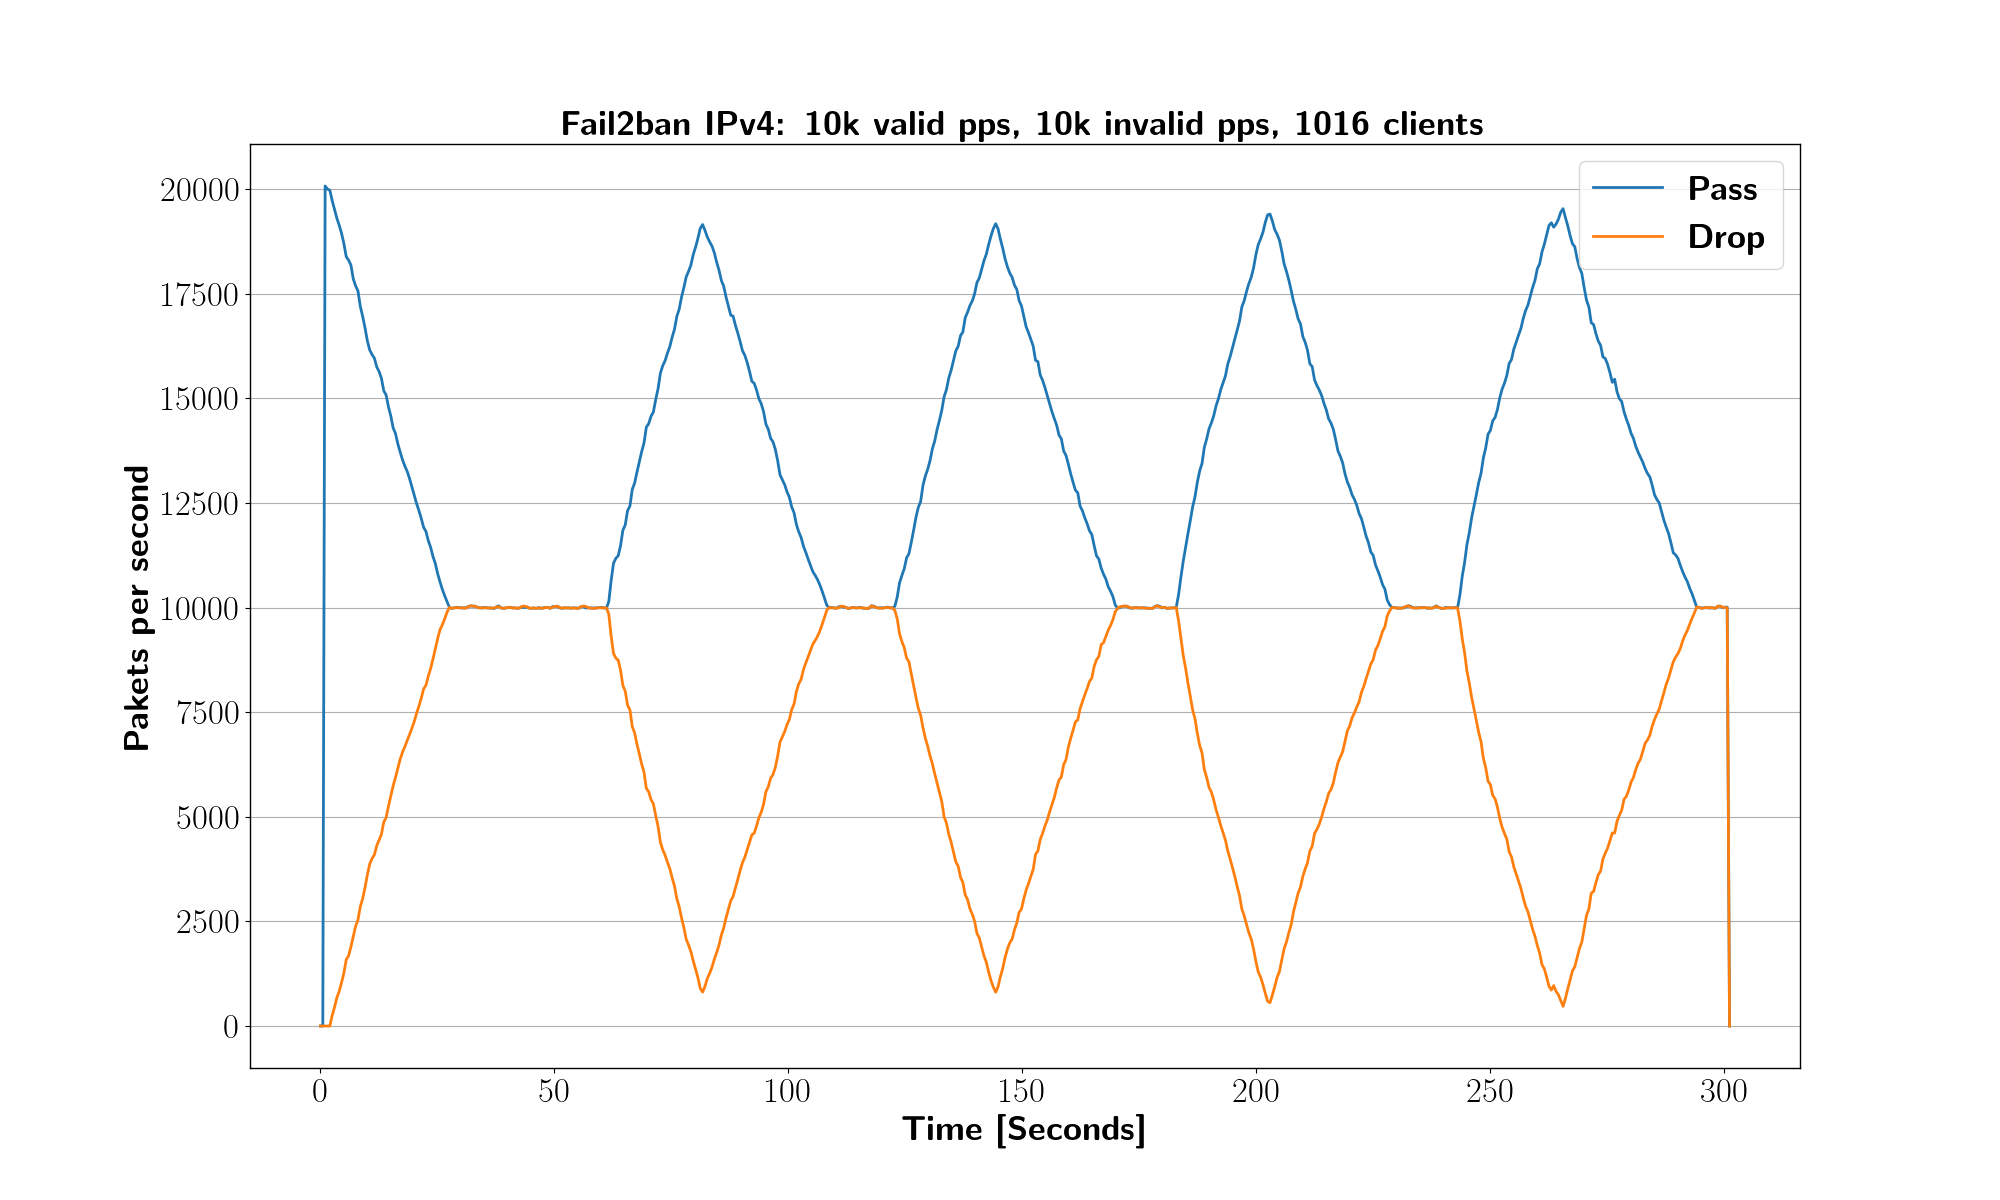
\includegraphics[width=1.2\textwidth]{images/fail2ban_v10k_iv10k_c1016.png}}
    \caption[Fail2Ban Replication Measurements 1]{Abstract architecture }
\end{figure}

\begin{figure}[p]
	\label{fig:fail2ban:1m}
    \centerline{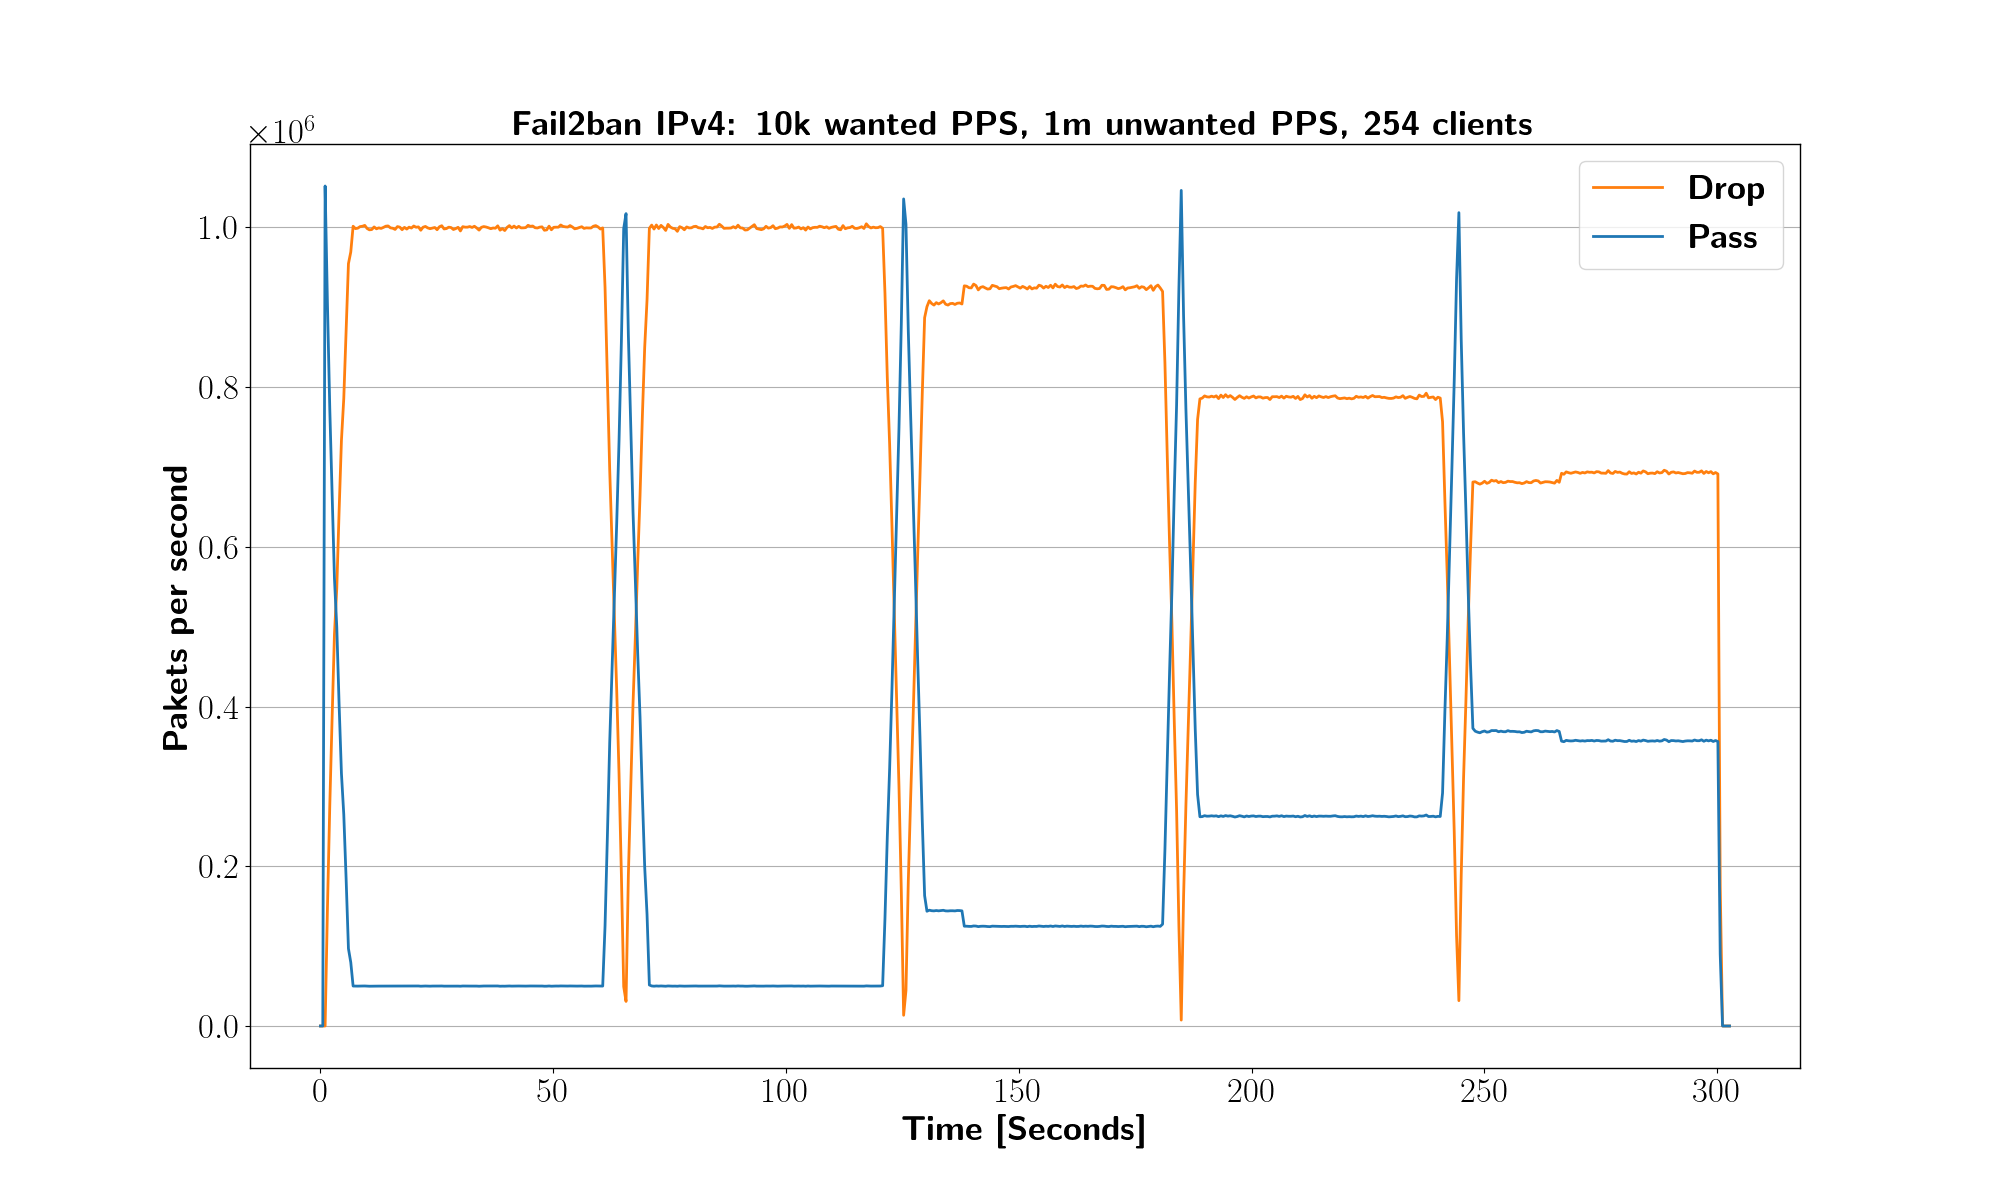
\includegraphics[width=1.2\textwidth]{images/fail2ban_v50k_iv1m_c254.png}}
    \caption[IPC Architecture]{Abstract architecture }
\end{figure}

\section{Simplefail2ban, Logfile Measurements}

\begin{figure}[p]
	\label{fig:simplefail2ban:disk:ip4:100k}
	\centering
	\scriptsize
	\begin{tabular}{c}
    	\centerline{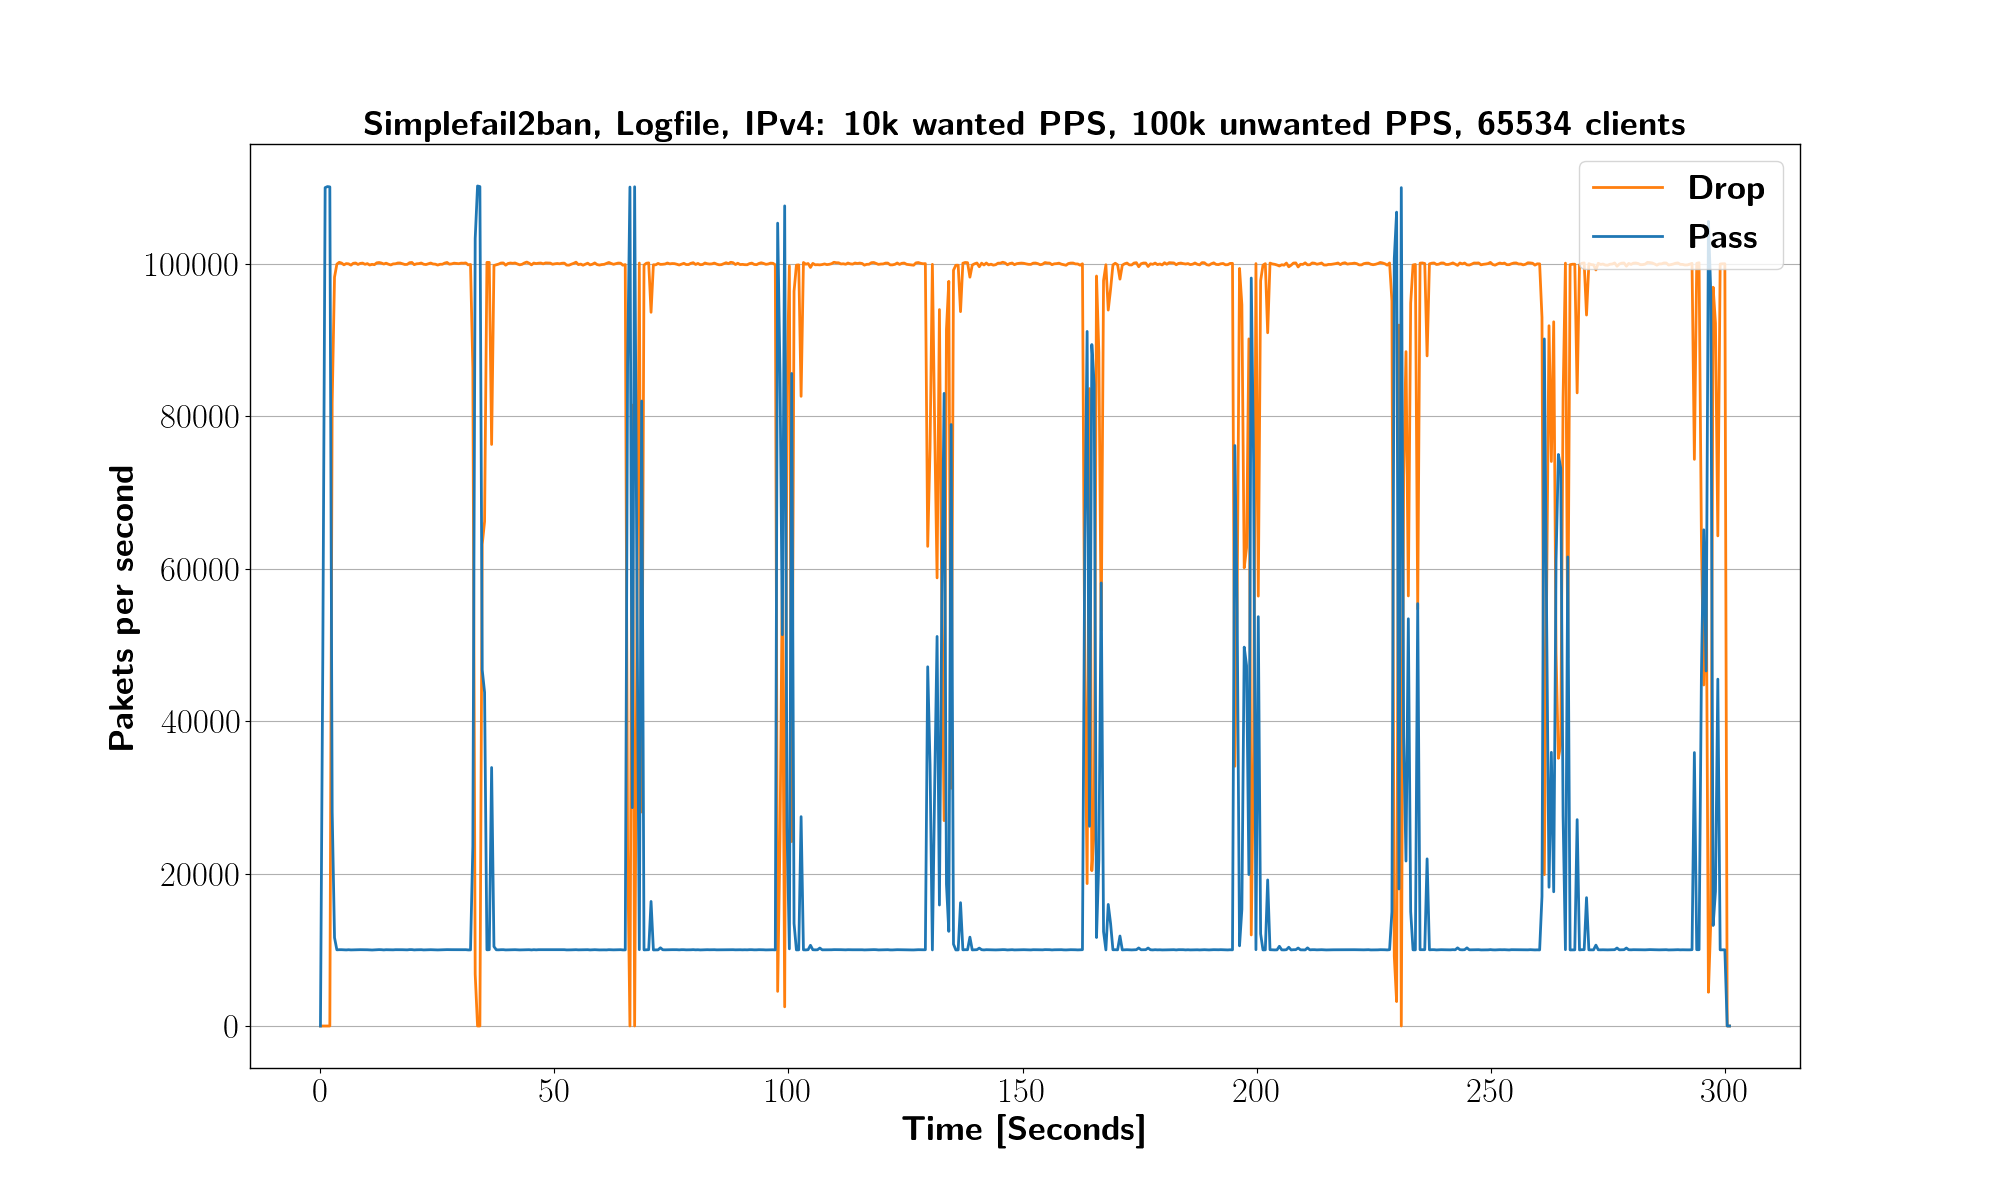
\includegraphics[width=1.2\textwidth]{images/simplefail2ban_disk_ipv4_v10k_iv100k_c65534.png}}
	\end{tabular}
	\begin{tabular}{lllll}
		\toprule
		\textbf{Total packets [$10^6$]} & \textbf{Packets dropped [$10^6$]} & \textbf{Relative drop [\%]} & \textbf{Log messages [$10^6$]} & \textbf{CPU [seconds]} \\ \midrule 
		33 & 27.93 & 99.59 & 2.07 & 10.51 \\
		\bottomrule
	\end{tabular}
	\caption[Simplefail2ban, Logfile IPv4, 100k \ac{PPS}]{Some text}
\end{figure}

\begin{figure}[p]
	\label{fig:simplefail2ban:disk:ip4:1m}
	\centering
	\scriptsize
	\begin{tabular}{c}
    	\centerline{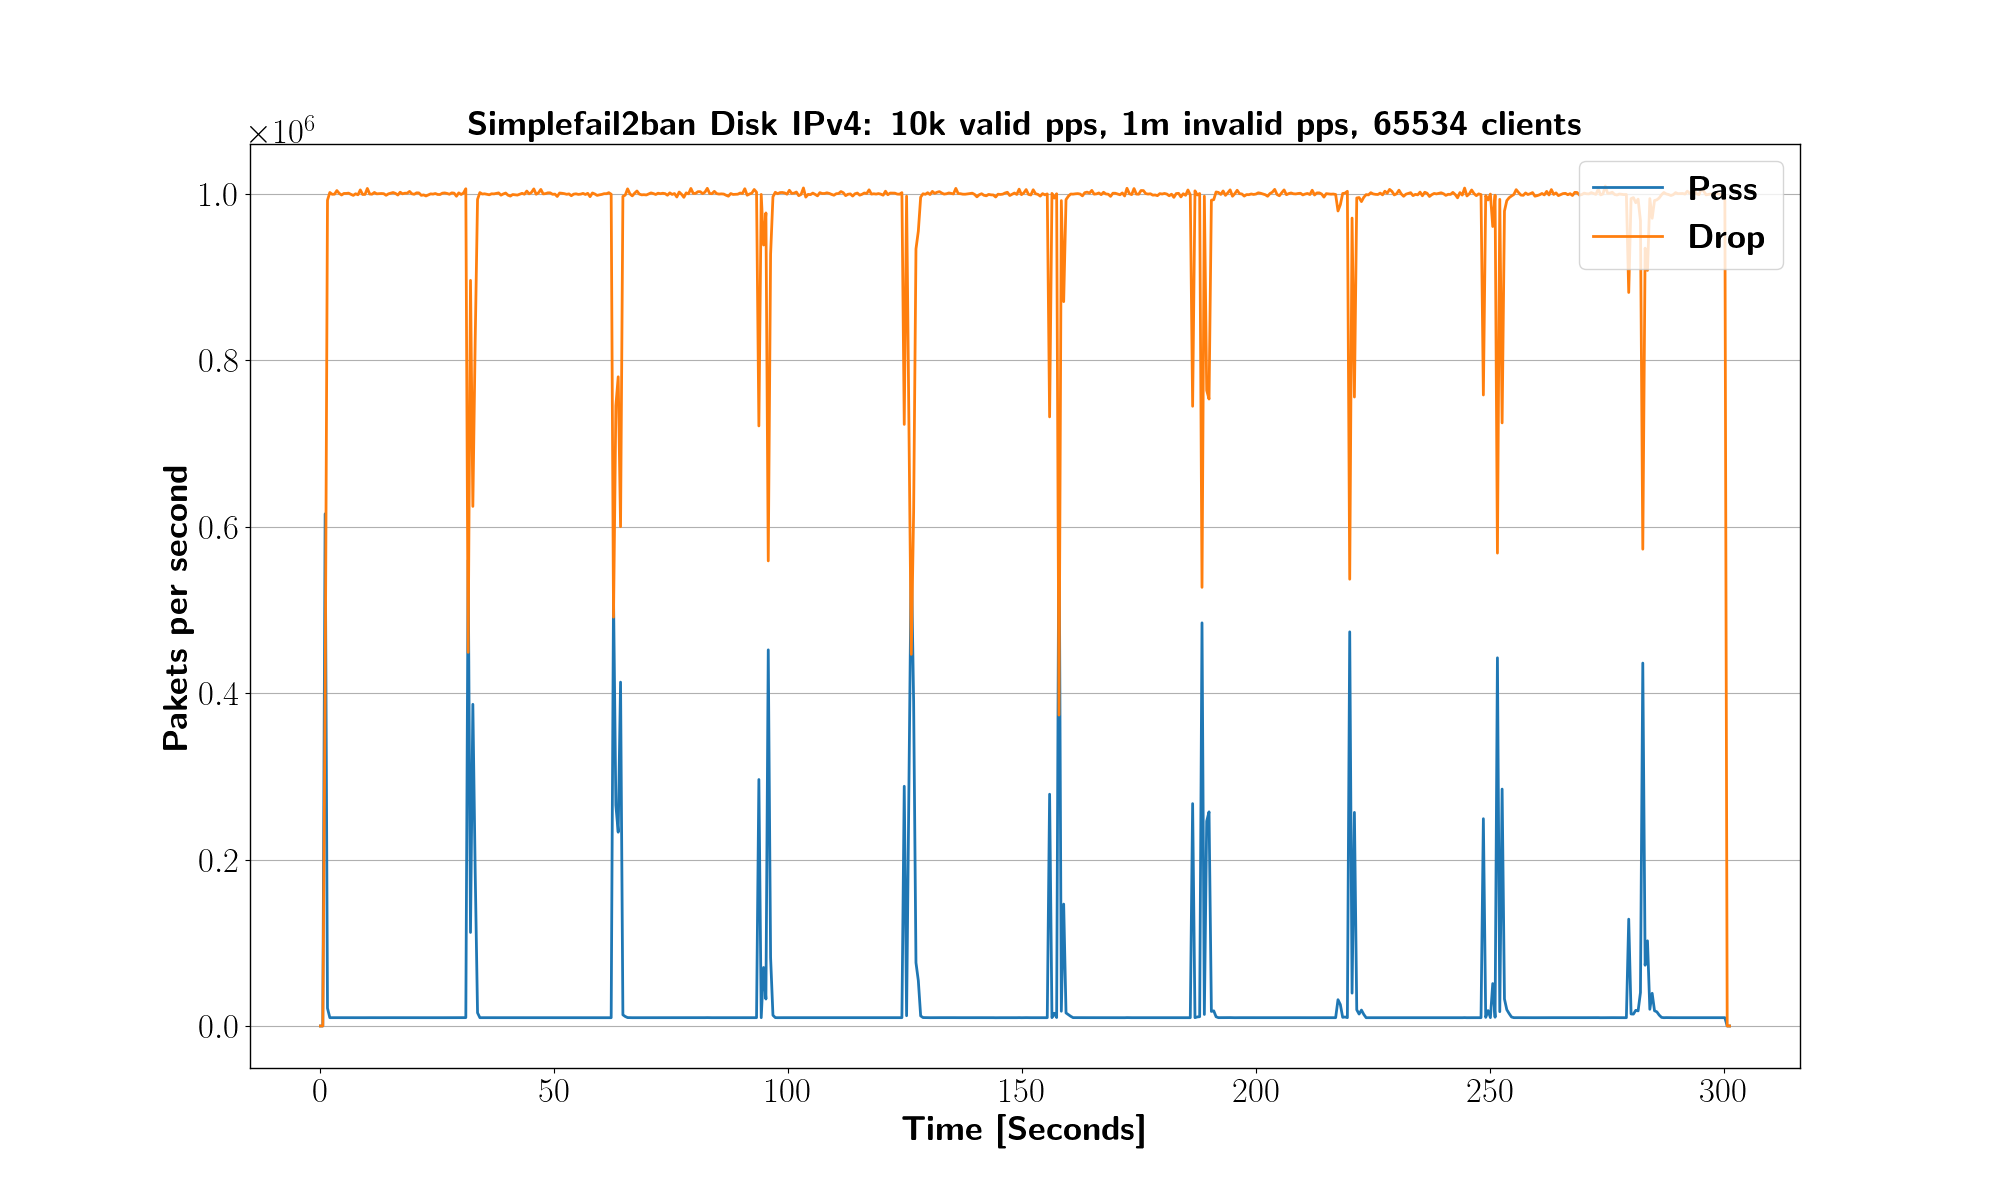
\includegraphics[width=1.2\textwidth]{images/simplefail2ban_disk_ipv4_v10k_iv1m_c65534.png}}
    \end{tabular}
	\begin{tabular}{lllll}
		\toprule
		\textbf{Total packets [$10^6$]} & \textbf{Packets dropped [$10^6$]} & \textbf{Relative drop [\%]} & \textbf{Log messages [$10^6$]} & \textbf{CPU [seconds]} \\ \midrule 
		303 & 294.43 & 98.79 & 4.7 & 14.99 \\
		\bottomrule
	\end{tabular}
	\caption[Simplefail2ban, Logfile IPv4, 1m \ac{PPS}]{Some text}
\end{figure}

\begin{figure}[p]
	\label{fig:simplefail2ban:disk:ip4:10m}
	\centering
	\scriptsize
	\begin{tabular}{c}
    	\centerline{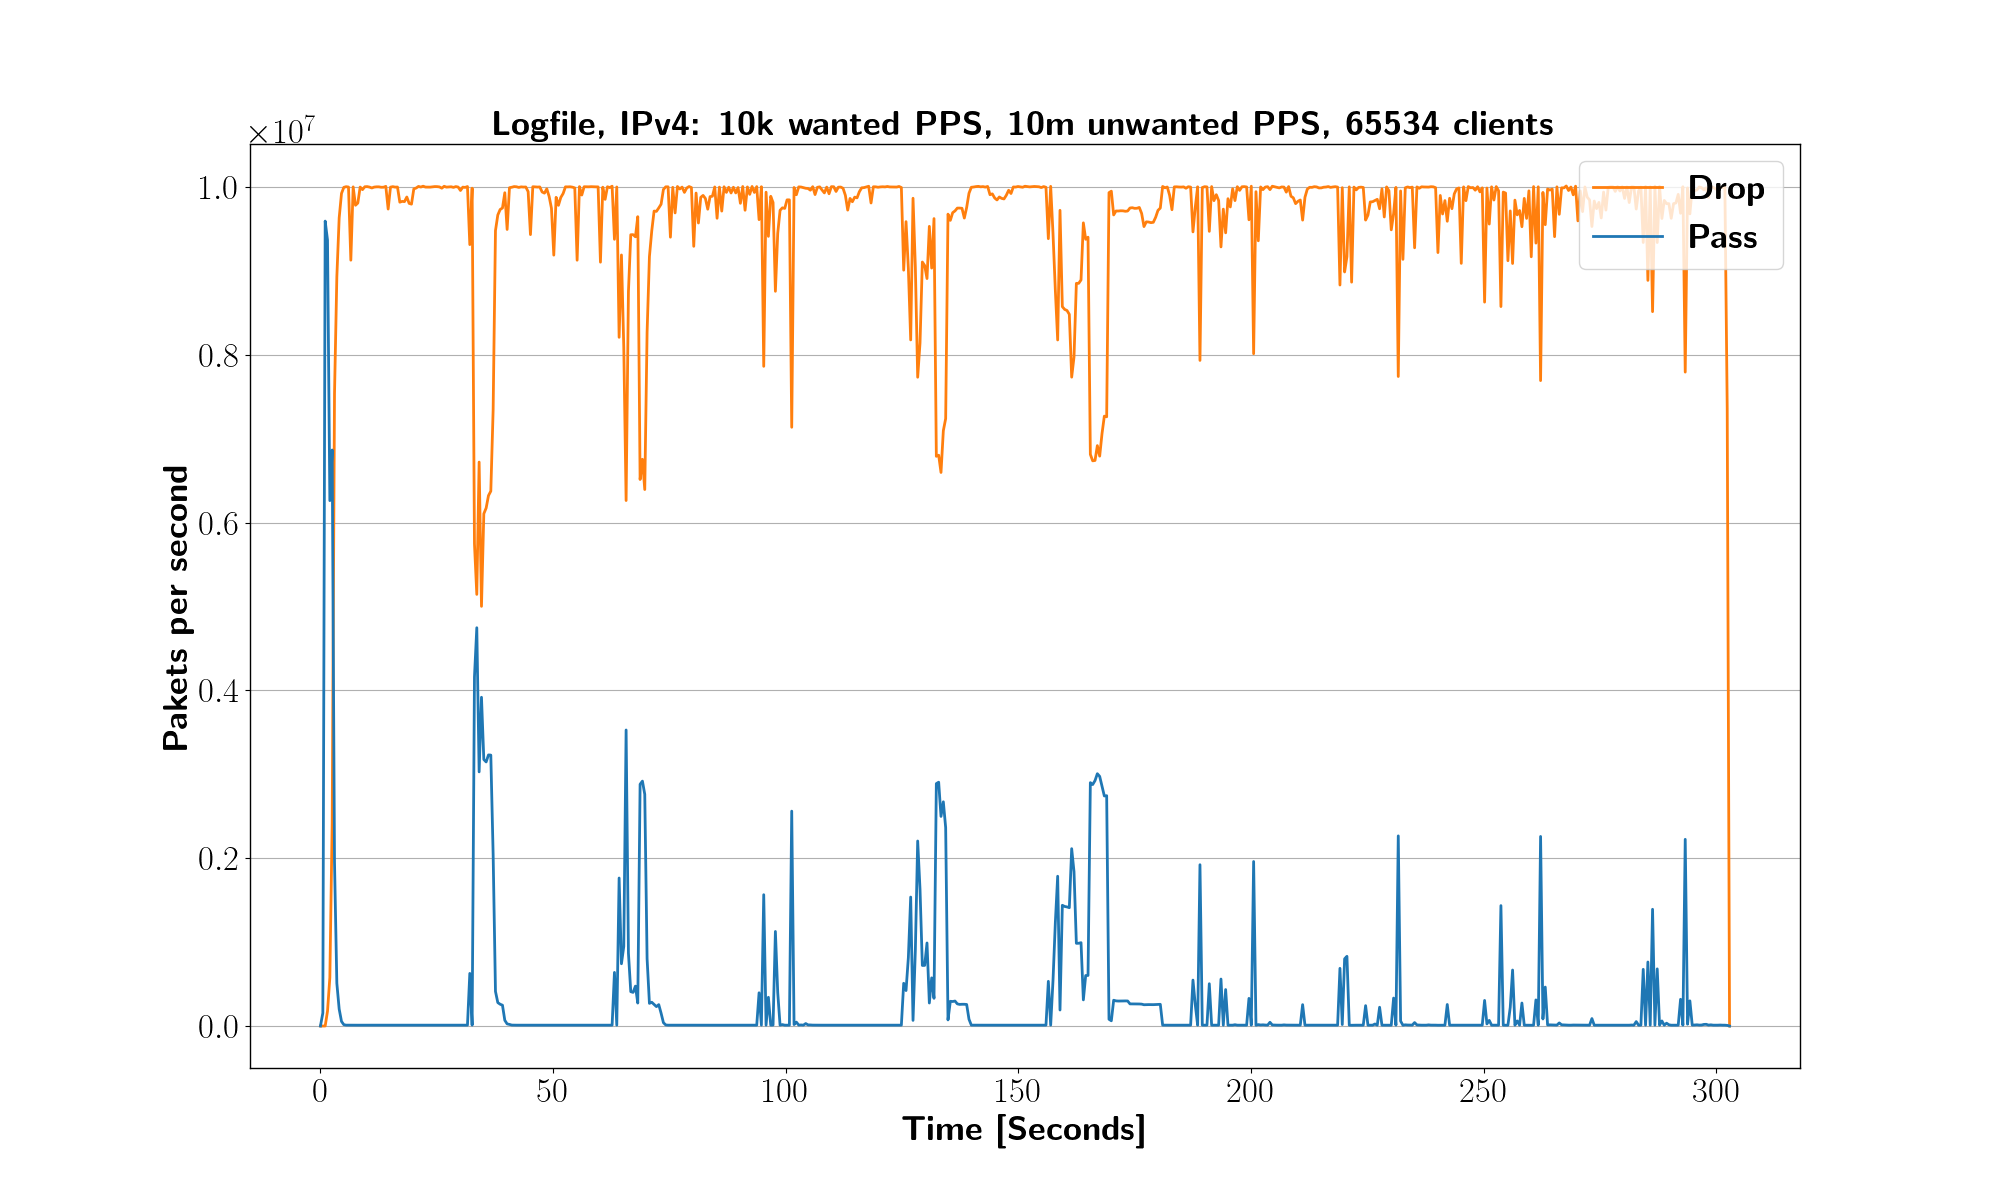
\includegraphics[width=1.2\textwidth]{images/simplefail2ban_disk_ipv4_v10k_iv10m_c65534.png}}
	\end{tabular}
	\begin{tabular}{lllll}
		\toprule
		\textbf{Total packets [$10^6$]} & \textbf{Packets dropped [$10^6$]} & \textbf{Relative drop [\%]} & \textbf{Log messages [$10^6$]} & \textbf{CPU [seconds]} \\ \midrule 
		2986.89 & 2884.14 & 96.72 & 34.39 & 83.72 \\
		\bottomrule
	\end{tabular}
	\caption[Simplefail2ban, Logfile IPv4, 10m \ac{PPS}]{Some text}
\end{figure}

\begin{figure}[p]
	\label{fig:simplefail2ban:disk:ip6:100k}
	\centering
	\scriptsize
	\begin{tabular}{c}
    	\centerline{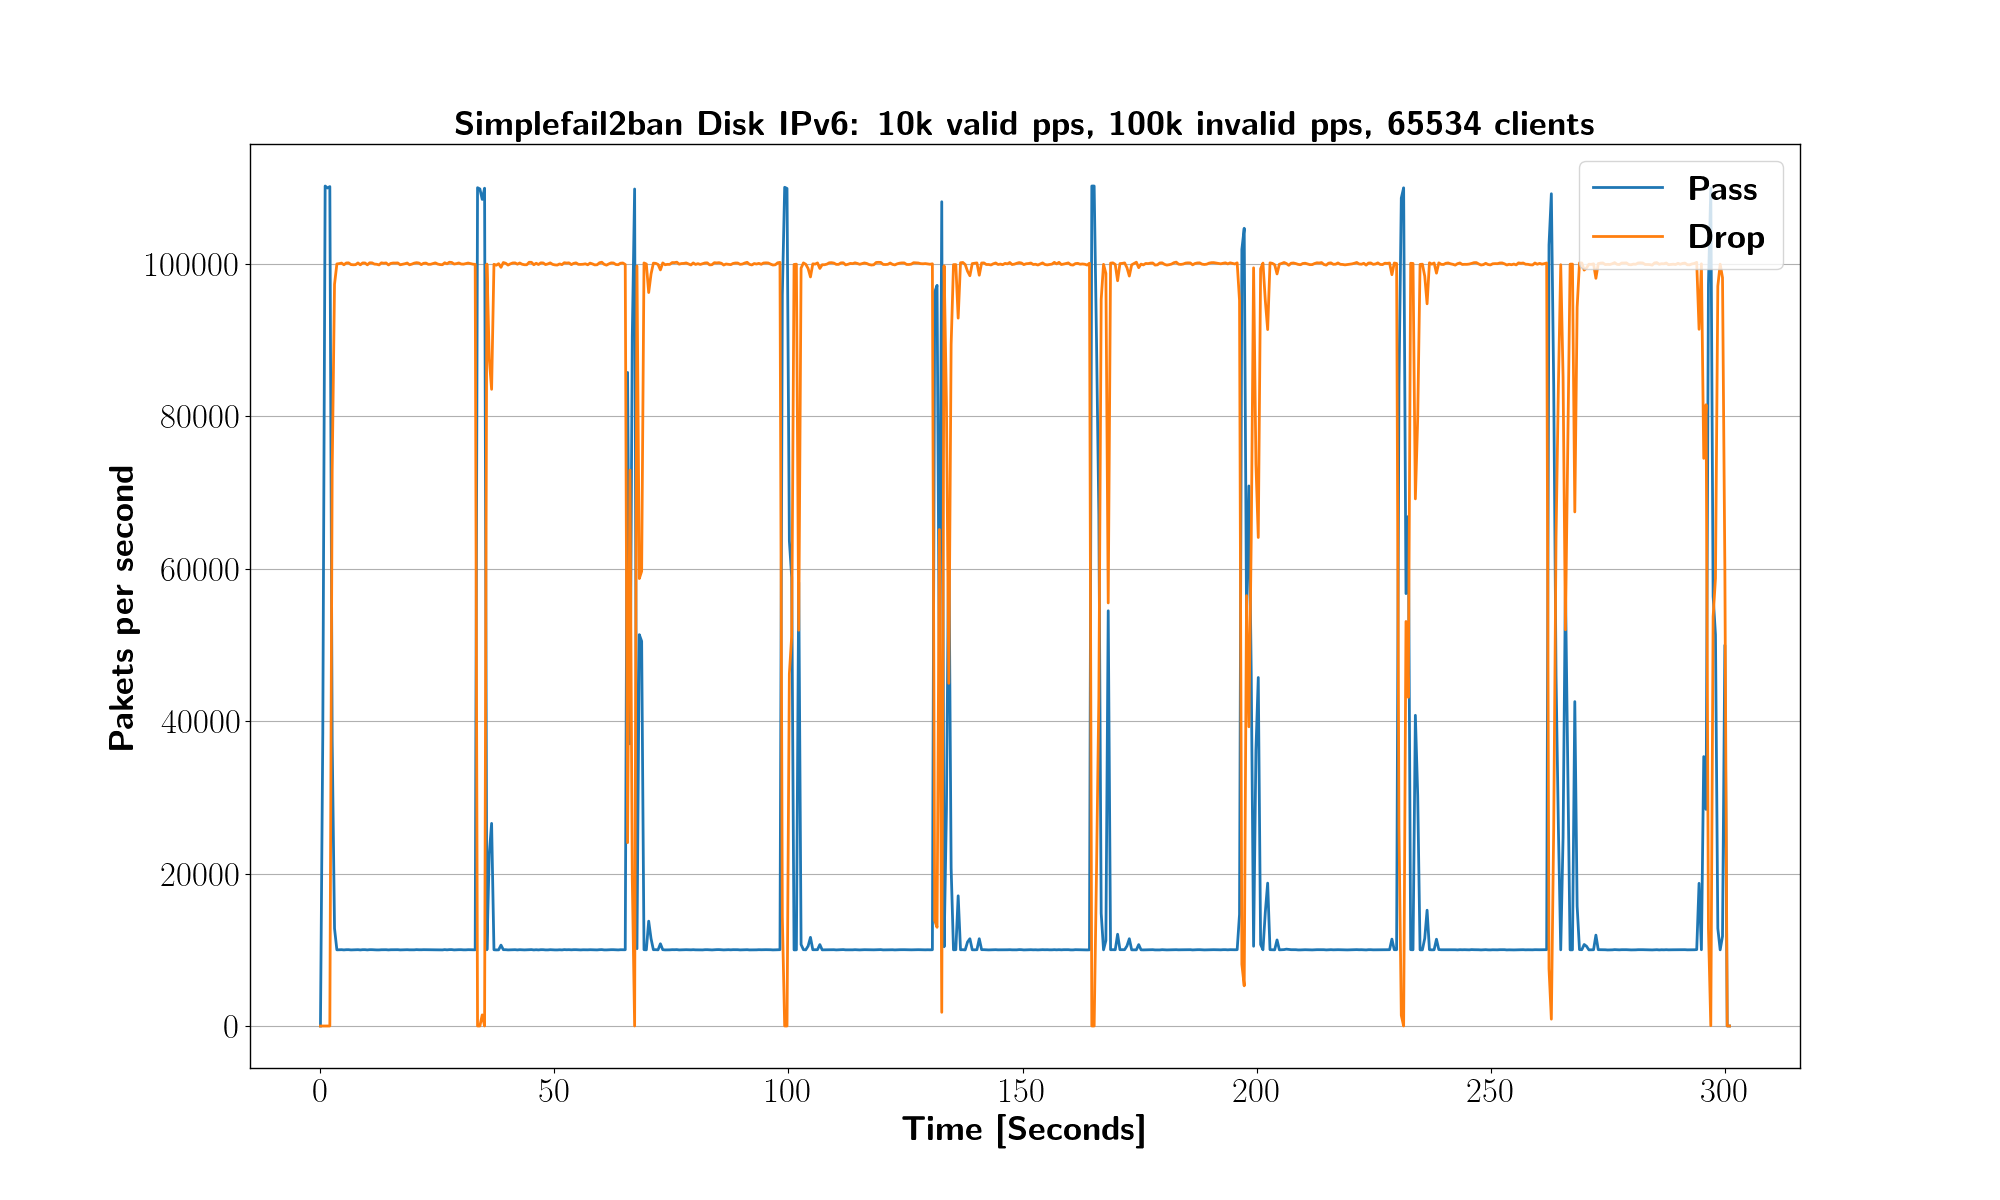
\includegraphics[width=1.2\textwidth]{images/simplefail2ban_disk_ipv6_v10k_iv100k_c65534.png}}
	\end{tabular}
	\begin{tabular}{lllll}
		\toprule
		\textbf{Total packets [$10^6$]} & \textbf{Packets dropped [$10^6$]} & \textbf{Relative drop [\%]} & \textbf{Log messages [$10^6$]} & \textbf{CPU [seconds]} \\ \midrule 
		33 & 27.96 & 99.67 & 2.04 & 11.75 \\
		\bottomrule
	\end{tabular}
	\caption[Simplefail2ban, Logfile IPv6, 100k \ac{PPS}]{Some text}
\end{figure}

\begin{figure}[p]
	\label{fig:simplefail2ban:disk:ip6:1m}
	\centering
	\scriptsize
	\begin{tabular}{c}
    	\centerline{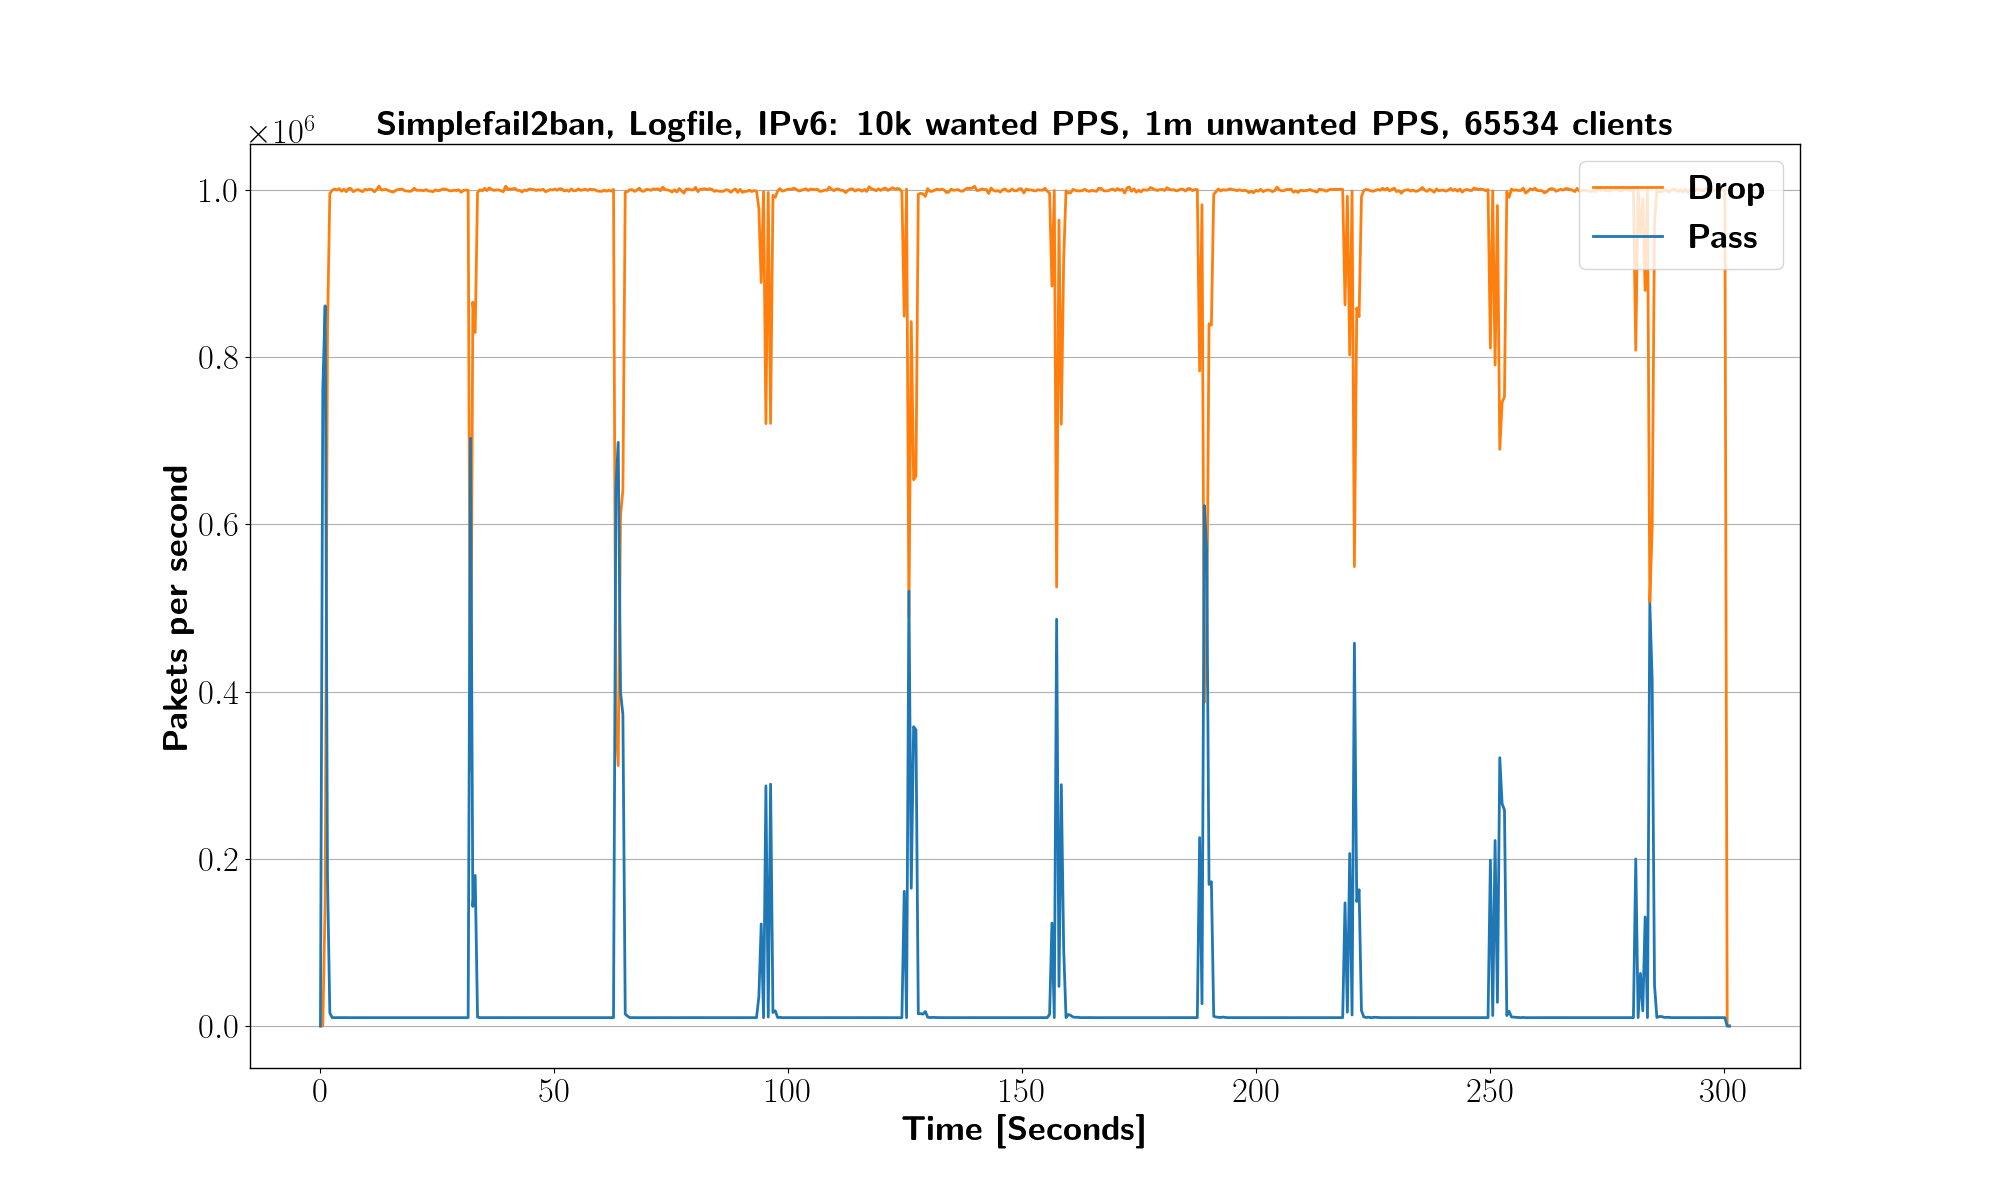
\includegraphics[width=1.2\textwidth]{images/simplefail2ban_disk_ipv6_v10k_iv1m_c65534.png}}
	\end{tabular}
	\begin{tabular}{lllll}
		\toprule
		\textbf{Total packets [$10^6$]} & \textbf{Packets dropped [$10^6$]} & \textbf{Relative drop [\%]} & \textbf{Log messages [$10^6$]} & \textbf{CPU [seconds]} \\ \midrule 
		303 & 293.49 & 98.48 & 5.58 & 21.08 \\
		\bottomrule
	\end{tabular}
	\caption[Simplefail2ban, Logfile IPv6, 1m \ac{PPS}]{Some text}
\end{figure}

\begin{figure}[p]
	\label{fig:simplefail2ban:disk:ip6:10m}
	\centering
	\scriptsize
	\begin{tabular}{c}
    	\centerline{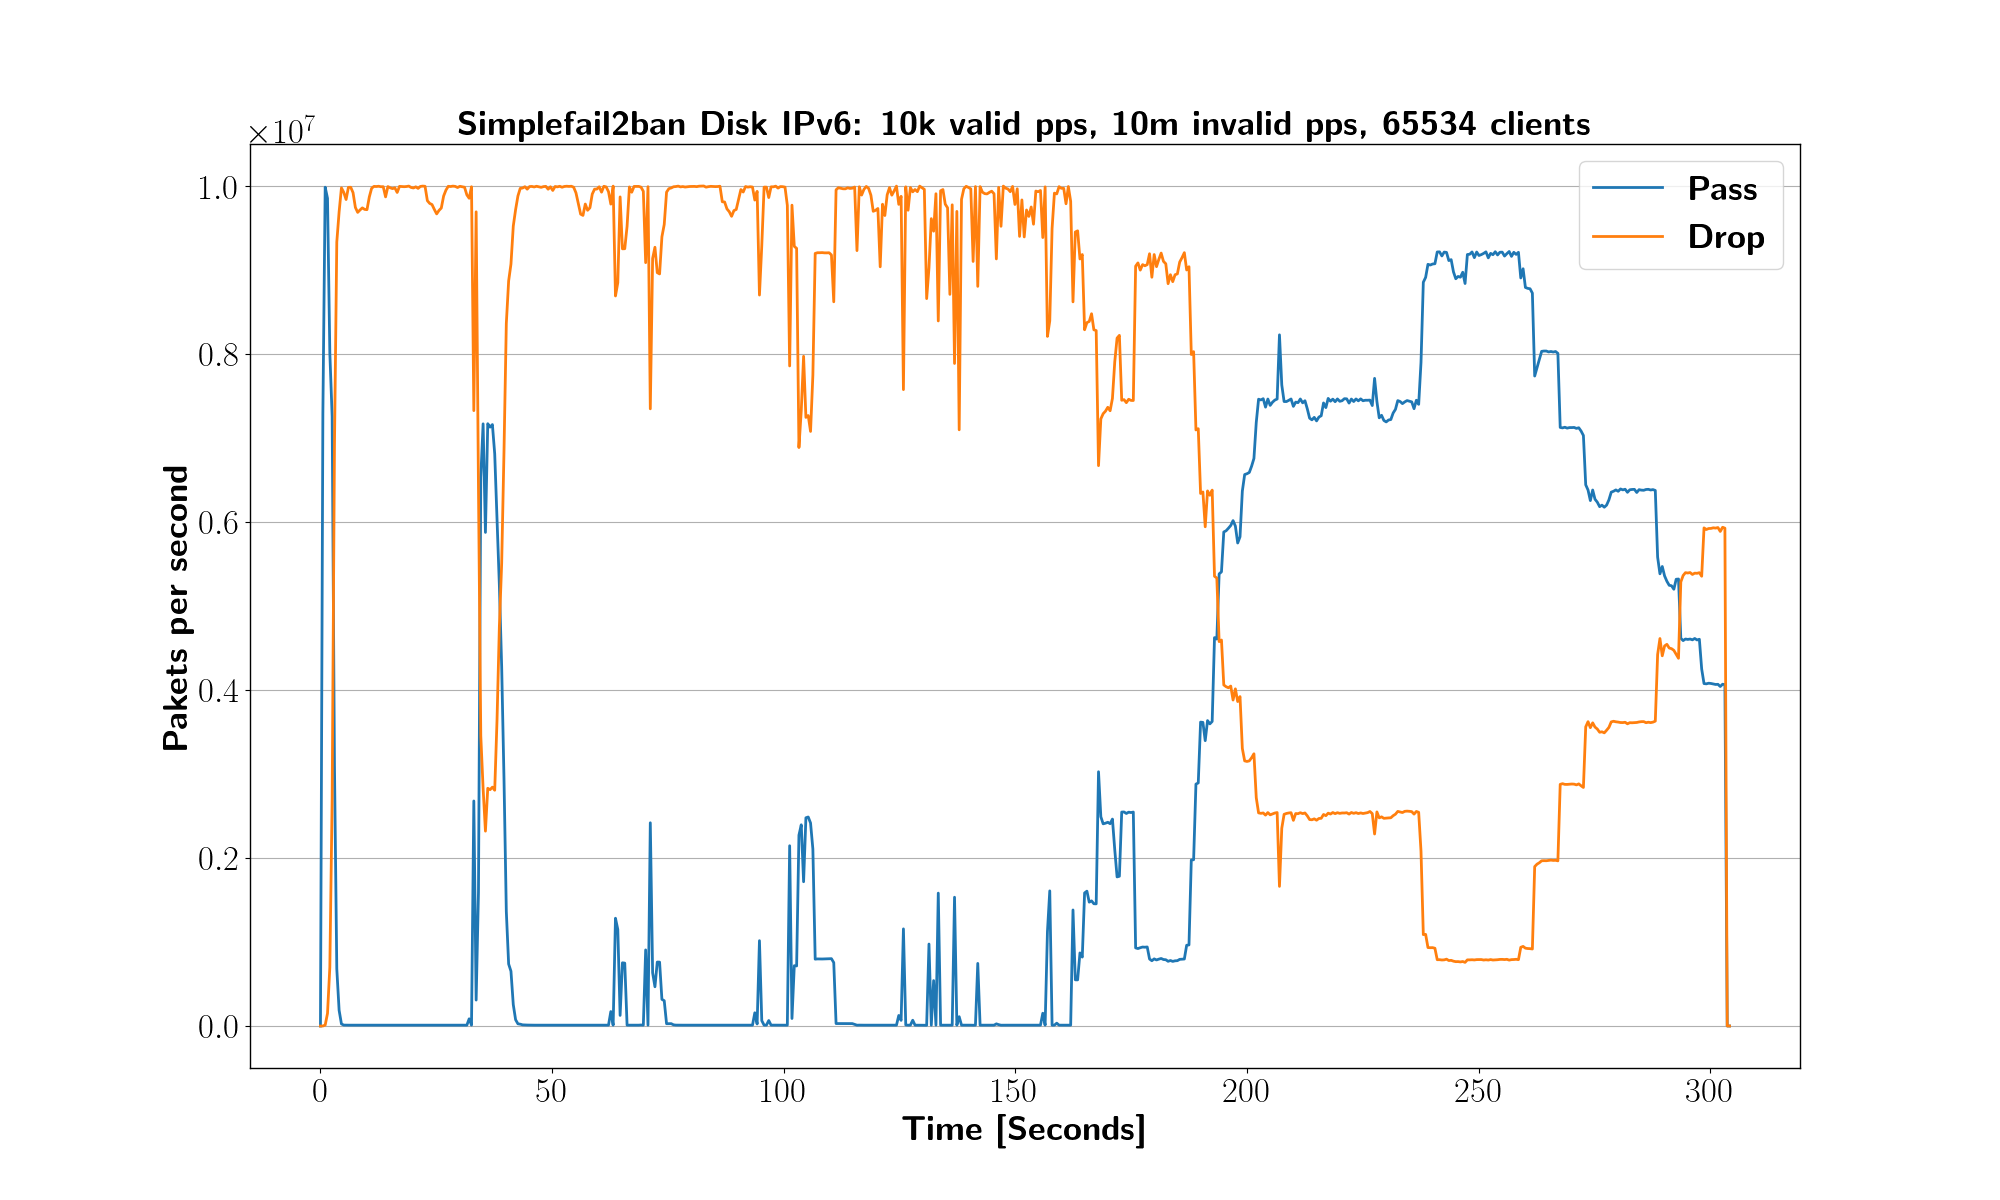
\includegraphics[width=1.2\textwidth]{images/simplefail2ban_disk_ipv6_v10k_iv10m_c65534.png}}
	\end{tabular}
	\begin{tabular}{lllll}
		\toprule
		\textbf{Total packets [$10^6$]} & \textbf{Packets dropped [$10^6$]} & \textbf{Relative drop [\%]} & \textbf{Log messages [$10^6$]} & \textbf{CPU [seconds]} \\ \midrule 
		2992.43 & 2065.28 & 69.13 & 205.4 & 346.73 \\
		\bottomrule
	\end{tabular}
	\caption[Simplefail2ban, Logfile IPv6, 10m \ac{PPS}]{Some text}
\end{figure}

\begin{figure}[p]
	\label{fig:simplefail2ban:disk:ip46:100k}
	\centering
	\scriptsize
	\begin{tabular}{c}
    	\centerline{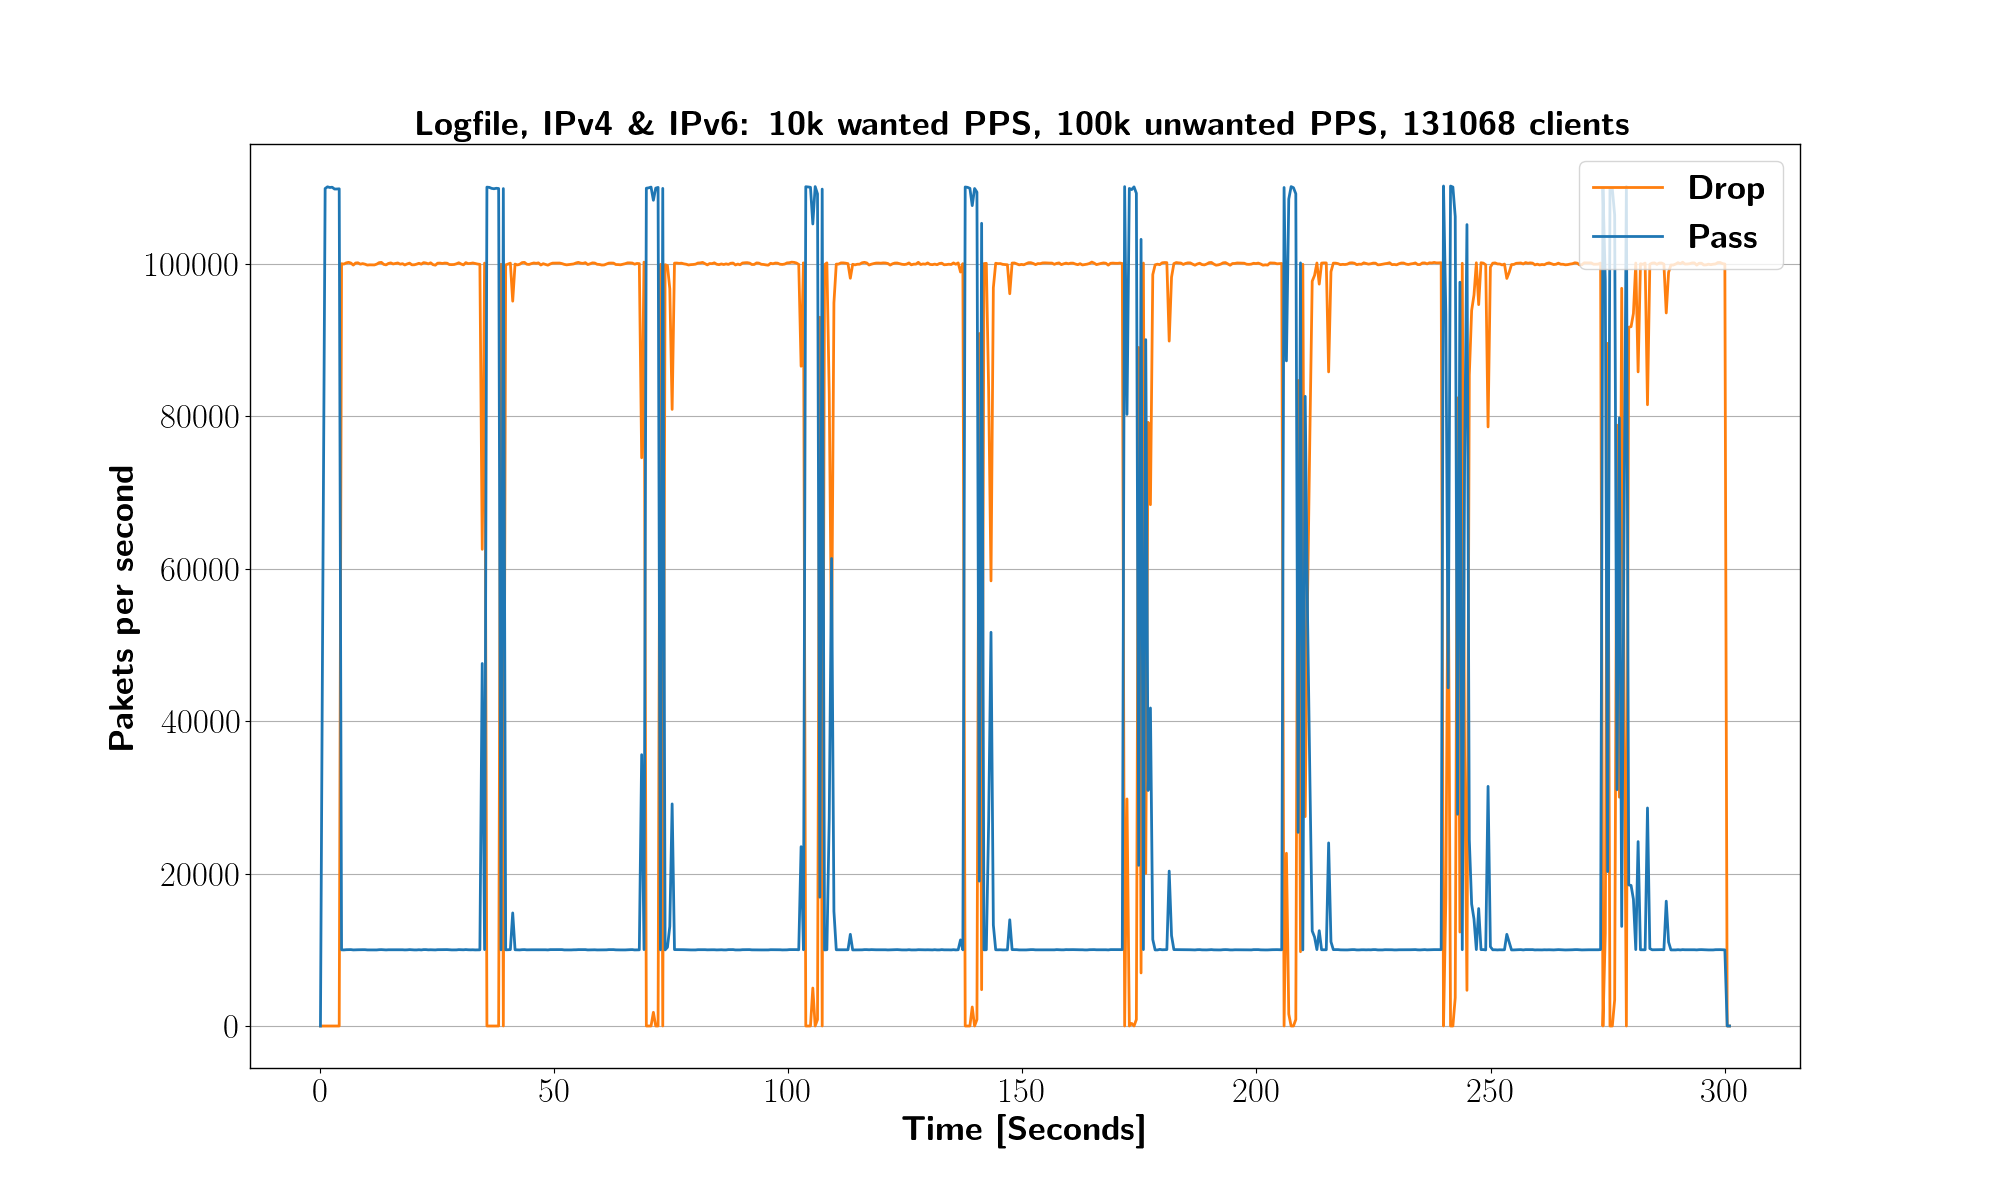
\includegraphics[width=1.2\textwidth]{images/simplefail2ban_disk_ipv46_v10k_iv100k_c131068.png}}
	\end{tabular}
	\begin{tabular}{lllll}
		\toprule
		\textbf{Total packets [$10^6$]} & \textbf{Packets dropped [$10^6$]} & \textbf{Relative drop [\%]} & \textbf{Log messages [$10^6$]} & \textbf{CPU [seconds]} \\ \midrule 
		33 & 26.45 & 99.96 & 3.55 & 18.47 \\
	\bottomrule
	\end{tabular}
	\caption[Simplefail2ban, Logfile IPv4 \& IPv6, 100k \ac{PPS}]{Some text}
\end{figure}

\begin{figure}[p]
	\label{fig:simplefail2ban:disk:ip46:1m}
	\centering
	\scriptsize
	\begin{tabular}{c}
    	\centerline{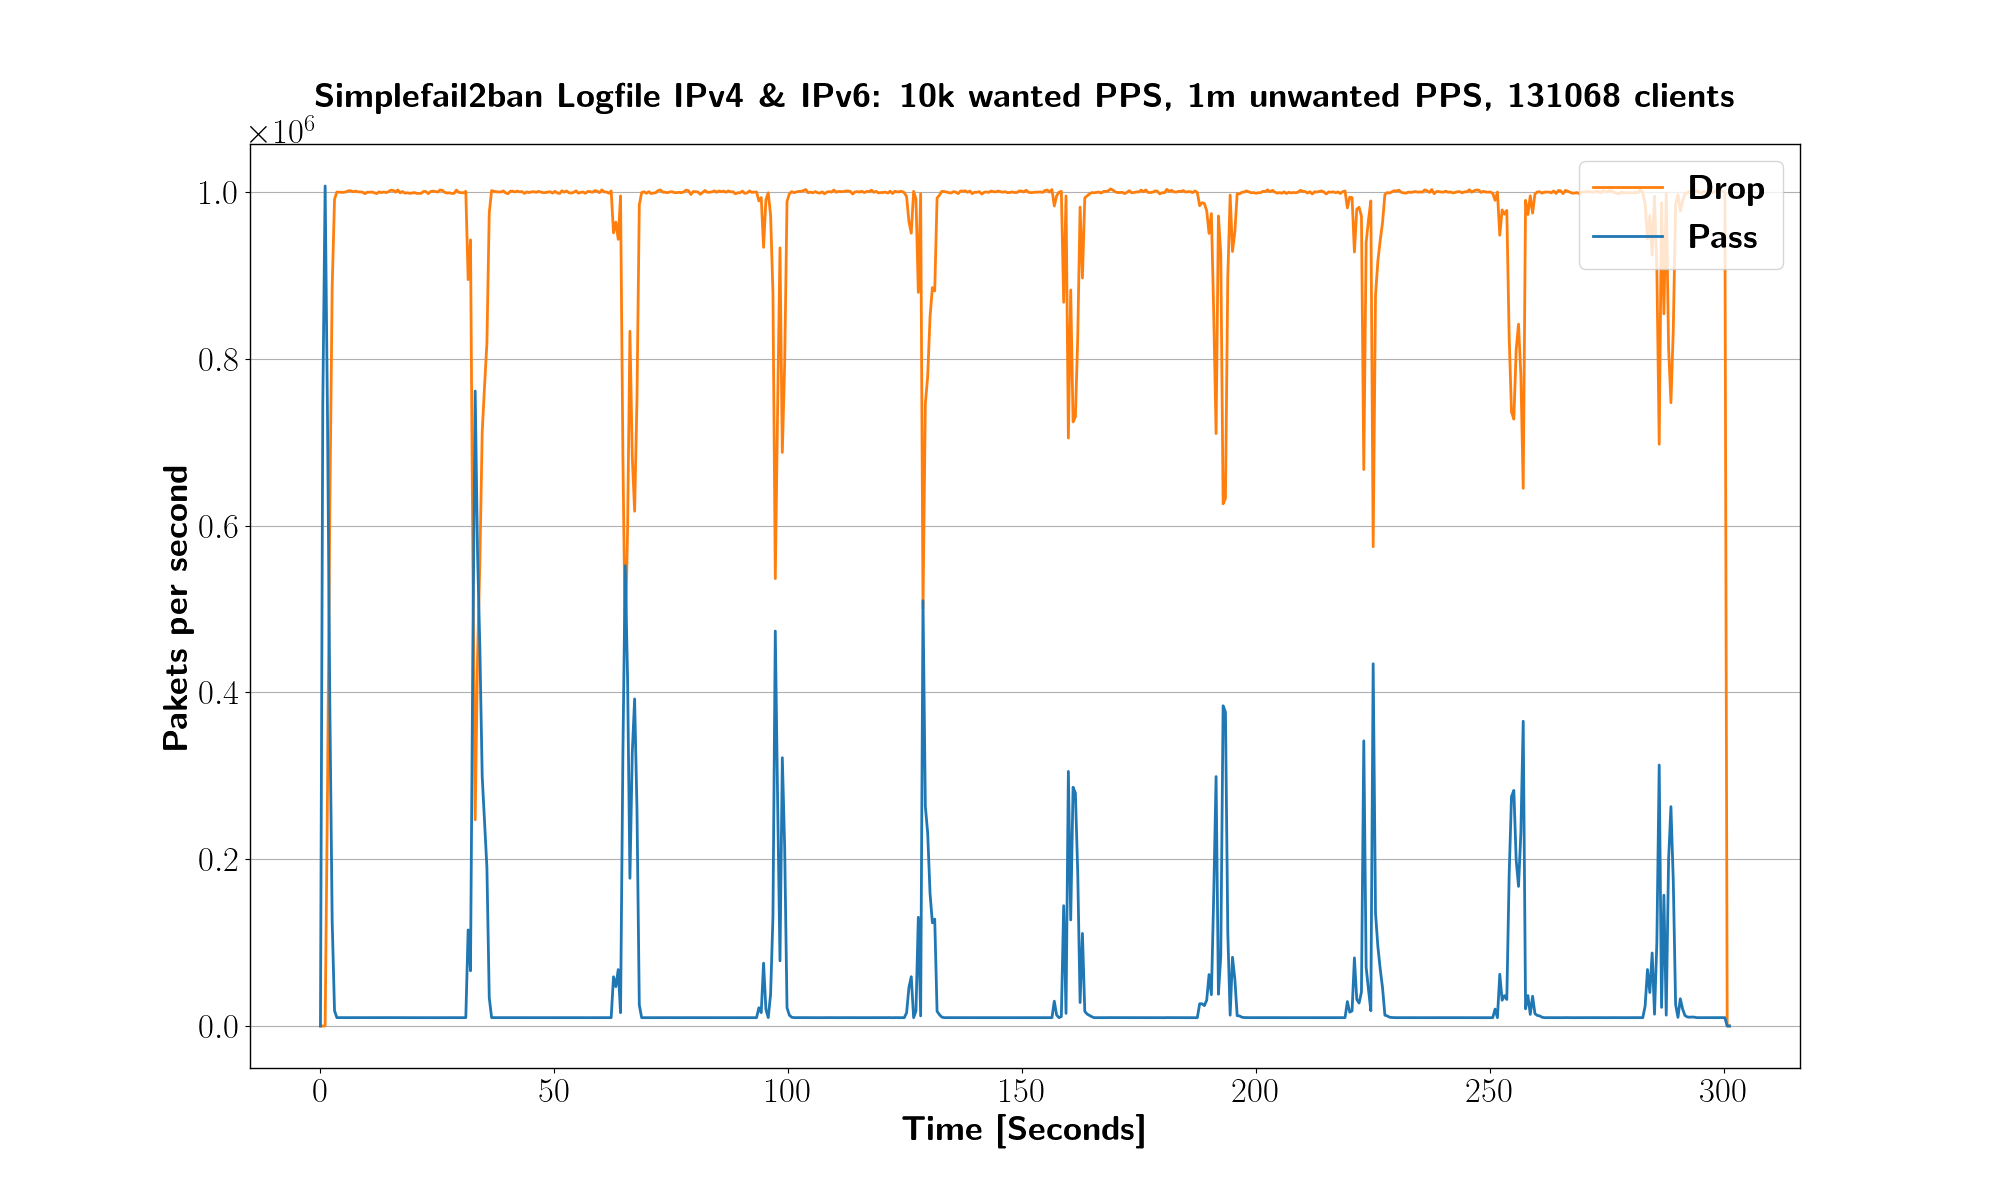
\includegraphics[width=1.2\textwidth]{images/simplefail2ban_disk_ipv46_v10k_iv1m_c131068.png}}
	\end{tabular}
	\begin{tabular}{lllll}
		\toprule
		\textbf{Total packets [$10^6$]} & \textbf{Packets dropped [$10^6$]} & \textbf{Relative drop [\%]} & \textbf{Log messages [$10^6$]} & \textbf{CPU [seconds]} \\ \midrule 
		303 & 290.47 & 98.11 & 8.5 & 32.94 \\
	\bottomrule
	\end{tabular}
	\caption[Simplefail2ban, Logfile IPv4 \& IPv6, 1m \ac{PPS}]{Some text}
\end{figure}

\begin{figure}[p]
	\label{fig:simplefail2ban:disk:ip46:10m}
	\centering
	\scriptsize
	\begin{tabular}{c}
    	\centerline{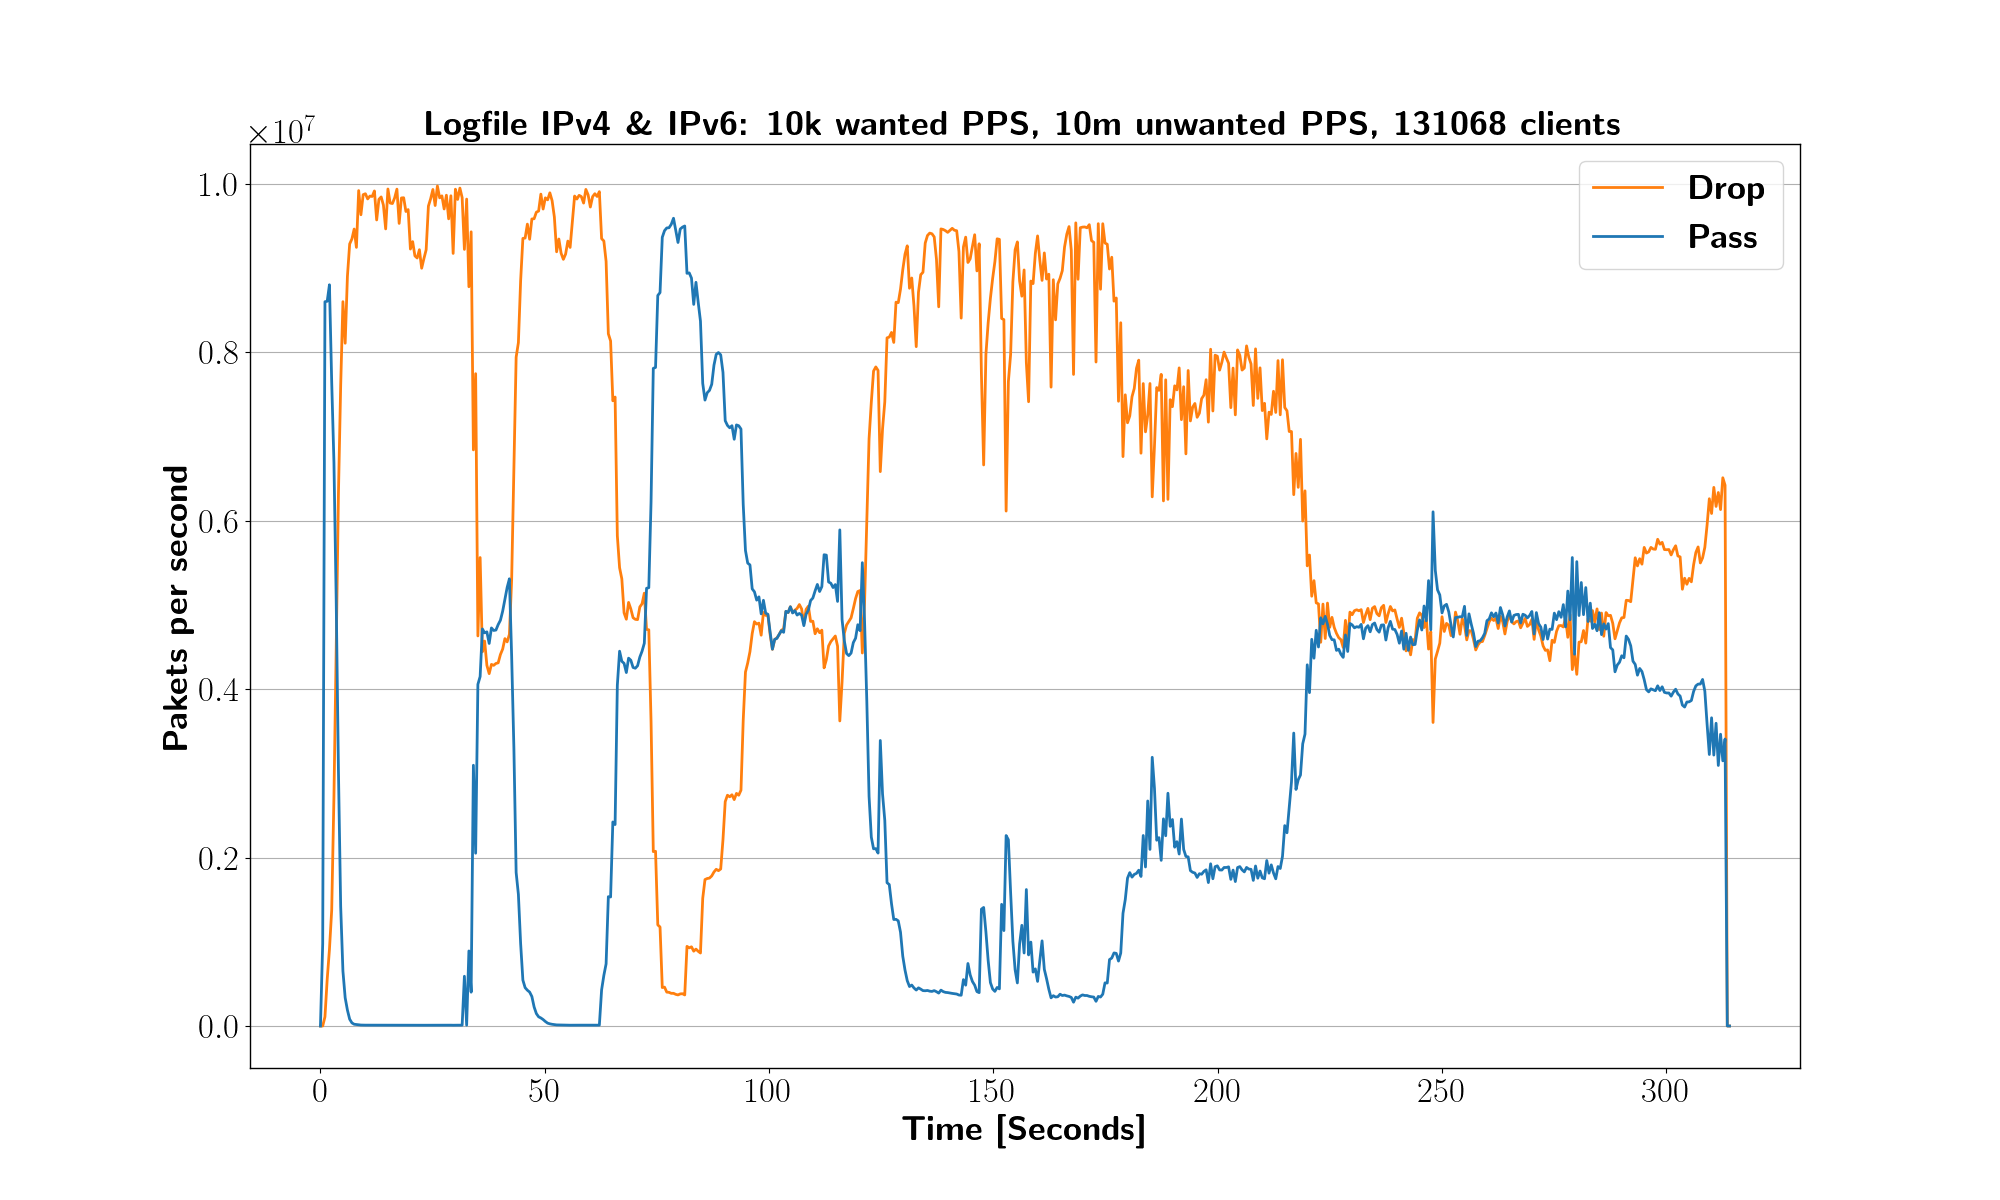
\includegraphics[width=1.2\textwidth]{images/simplefail2ban_disk_ipv46_v10k_iv10m_c131068.png}}
	\end{tabular}
	\begin{tabular}{lllll}
		\toprule
		\textbf{Total packets [$10^6$]} & \textbf{Packets dropped [$10^6$]} & \textbf{Relative drop [\%]} & \textbf{Log messages [$10^6$]} & \textbf{CPU [seconds]} \\ \midrule 
		2993.57 & 2014.77 & 67.46 & 213.63 & 382.19 \\
		\bottomrule
	\end{tabular}
	\caption[Simplefail2ban, Logfile IPv4 \& IPv6, 10m \ac{PPS}]{Some text}
\end{figure}

\section{Simplefail2ban, Shared Memory Measurements}

\begin{figure}[p]
	\label{fig:simplefail2ban:shm:ip4:100k}
	\centering
	\scriptsize
	\begin{tabular}{c}
    	\centerline{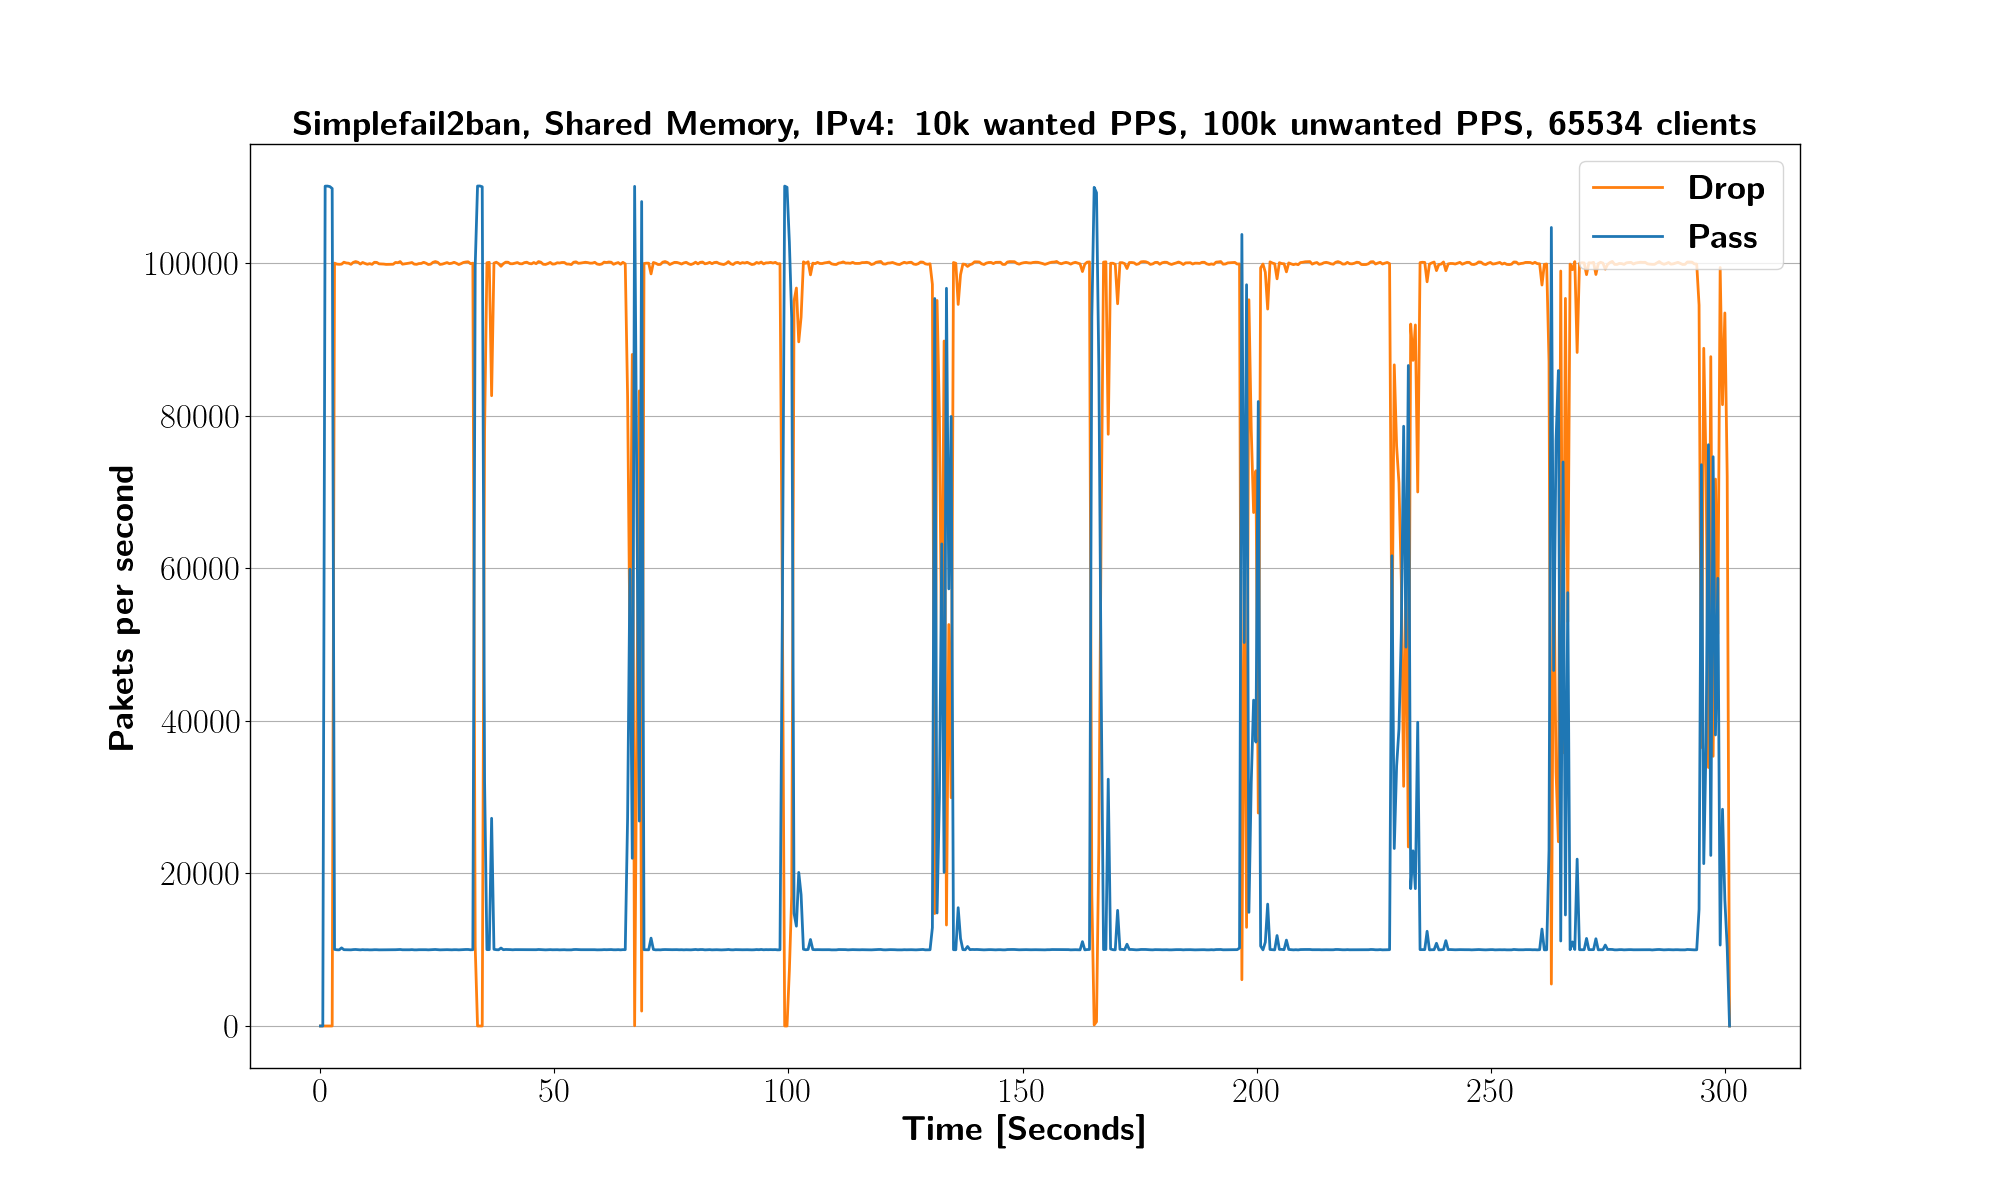
\includegraphics[width=1.2\textwidth]{images/simplefail2ban_shm_ipv4_v10k_iv100k_c65534.png}}
	\end{tabular}
	\begin{tabular}{lllll}
		\toprule
		\textbf{Total packets [$10^6$]} & \textbf{Packets dropped [$10^6$]} & \textbf{Relative drop [\%]} & \textbf{Log messages [$10^6$]} & \textbf{CPU [seconds]} \\ \midrule 
		33 & 27.95 & 99.64 & 2.05 & 13.68 \\
		\bottomrule
	\end{tabular}
	\caption[Simplefail2ban, Shared Memory, IPv4, 1m \ac{PPS}]{Some text}
\end{figure}

\begin{figure}[p]
	\label{fig:simplefail2ban:shm:ip4:1m}
	\centering
	\scriptsize
	\begin{tabular}{c}
    	\centerline{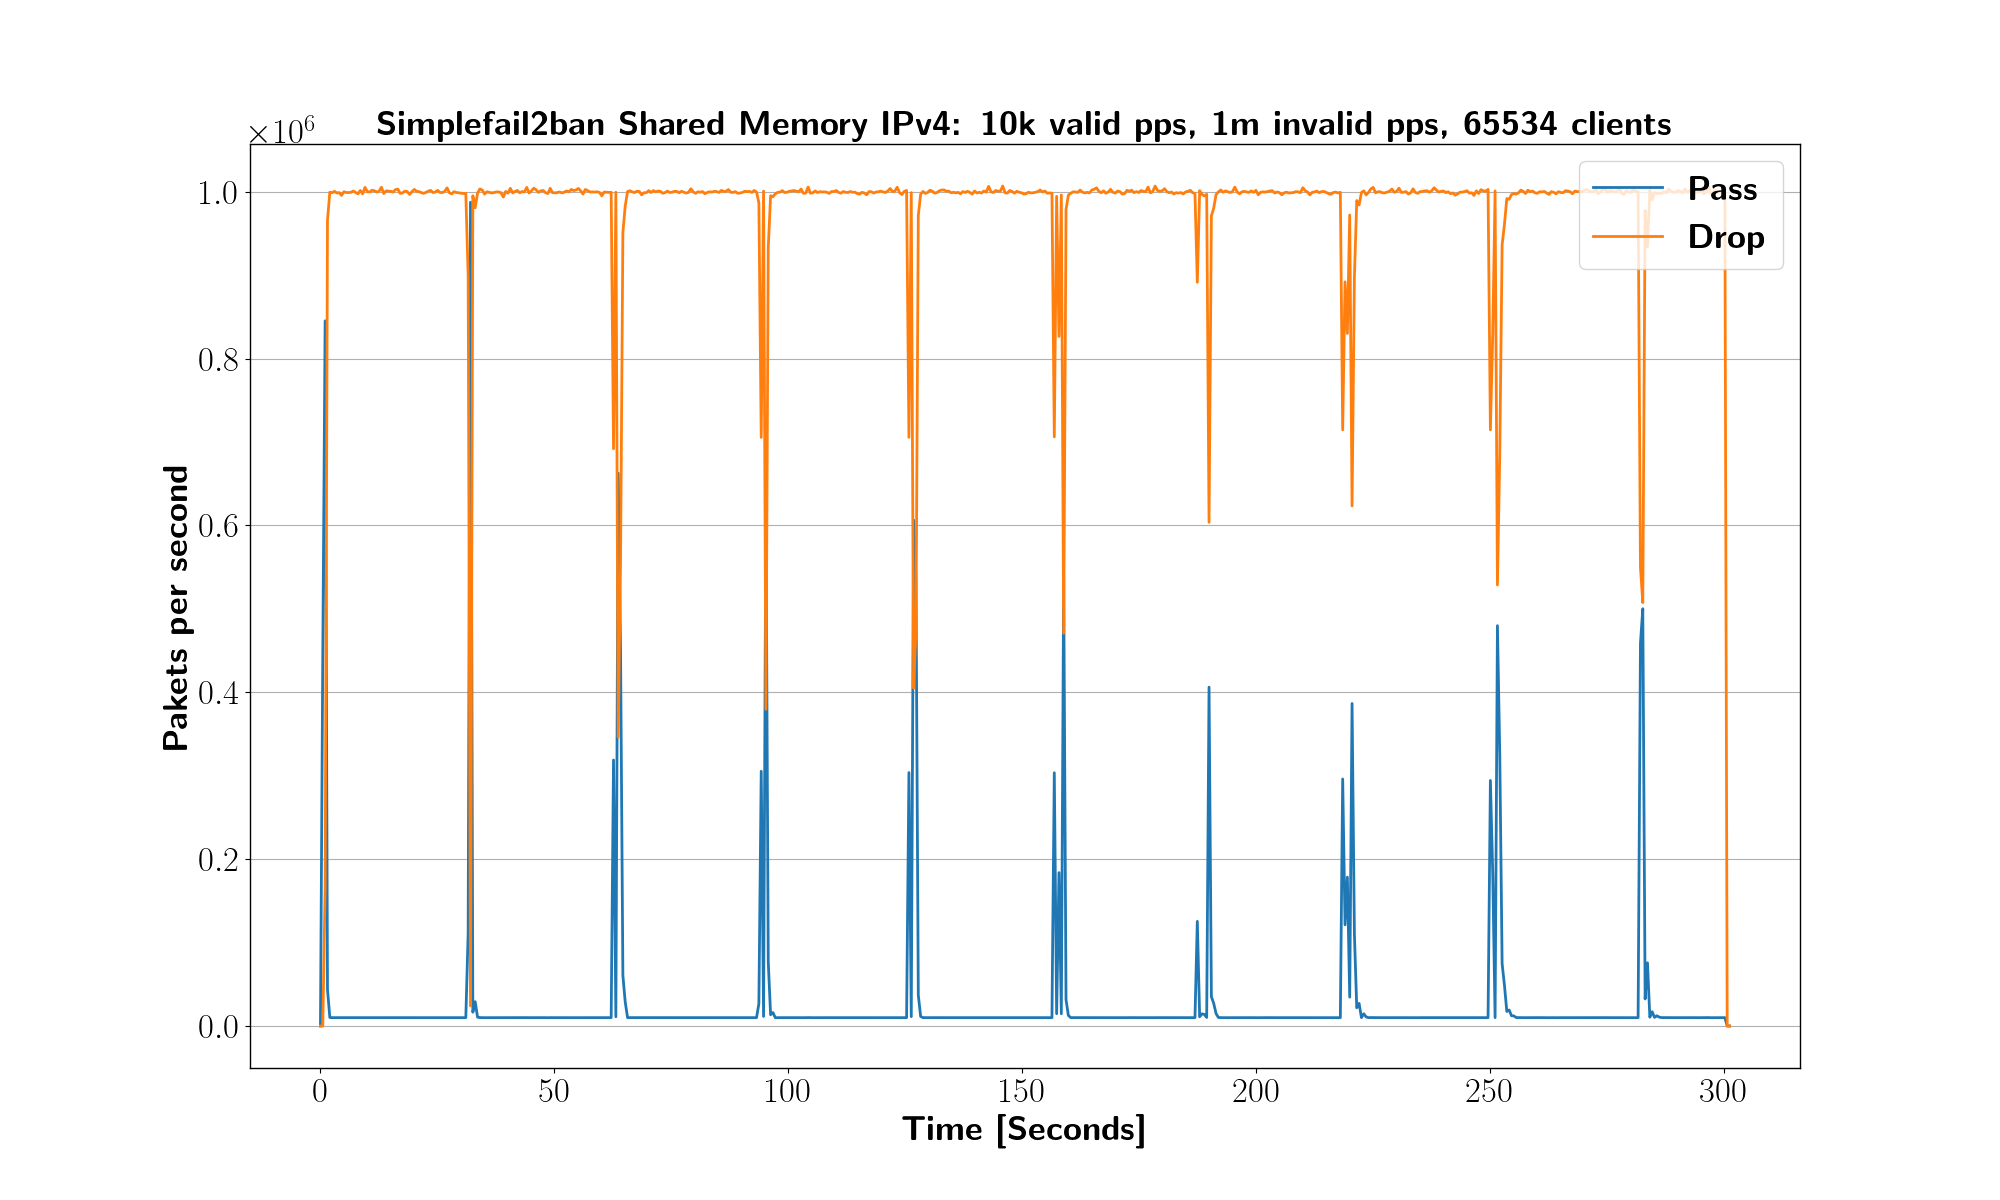
\includegraphics[width=1.2\textwidth]{images/simplefail2ban_shm_ipv4_v10k_iv1m_c65534.png}}
	\end{tabular}
	\begin{tabular}{lllll}
		\toprule
		\textbf{Total packets [$10^6$]} & \textbf{Packets dropped [$10^6$]} & \textbf{Relative drop [\%]} & \textbf{Log messages [$10^6$]} & \textbf{CPU [seconds]} \\ \midrule 
		303 & 294.34 & 98.88 & 4.61 & 15.52 \\
		\bottomrule
	\end{tabular}
	\caption[Simplefail2ban, Shared Memory, IPv4, 1m \ac{PPS}]{Some text}
\end{figure}

\begin{figure}[p]
	\label{fig:simplefail2ban:shm:ip4:10m}
	\centering
	\scriptsize
	\begin{tabular}{c}
    	\centerline{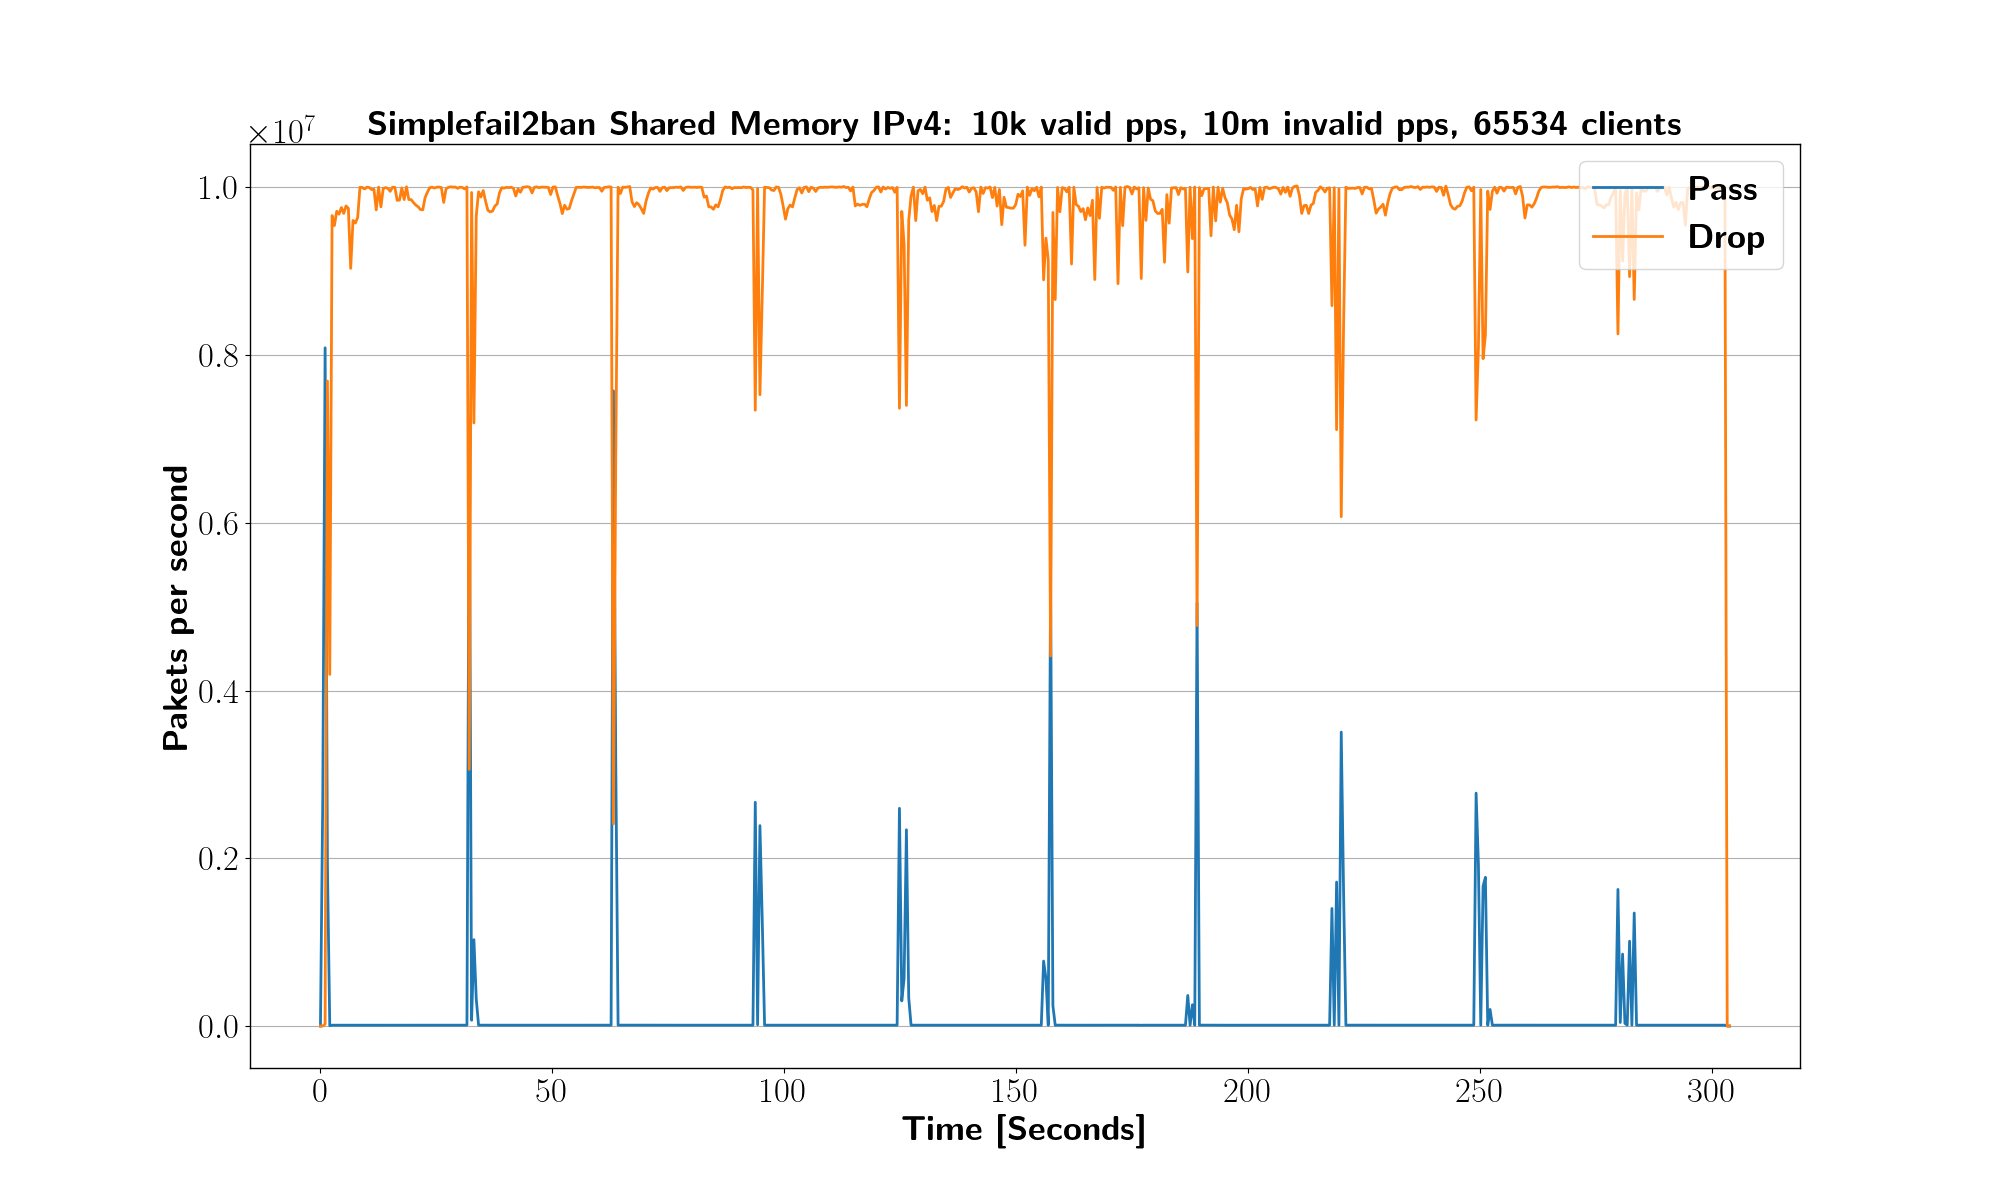
\includegraphics[width=1.2\textwidth]{images/simplefail2ban_shm_ipv4_v10k_iv10m_c65534.png}}
	\end{tabular}
	\begin{tabular}{lllll}
		\toprule
		\textbf{Total packets [$10^6$]} & \textbf{Packets dropped [$10^6$]} & \textbf{Relative drop [\%]} & \textbf{Log messages [$10^6$]} & \textbf{CPU [seconds]} \\ \midrule 
		2991.48 & 2948.51 & 96.72 & 7.69 & 25.59 \\
		\bottomrule
	\end{tabular}
	\caption[Simplefail2ban, Shared Memory, IPv4, 10m \ac{PPS}]{Some text}
\end{figure}

\begin{figure}[p]
	\label{fig:simplefail2ban:shm:ip6:100k}
	\centering
	\scriptsize
	\begin{tabular}{c}
    	\centerline{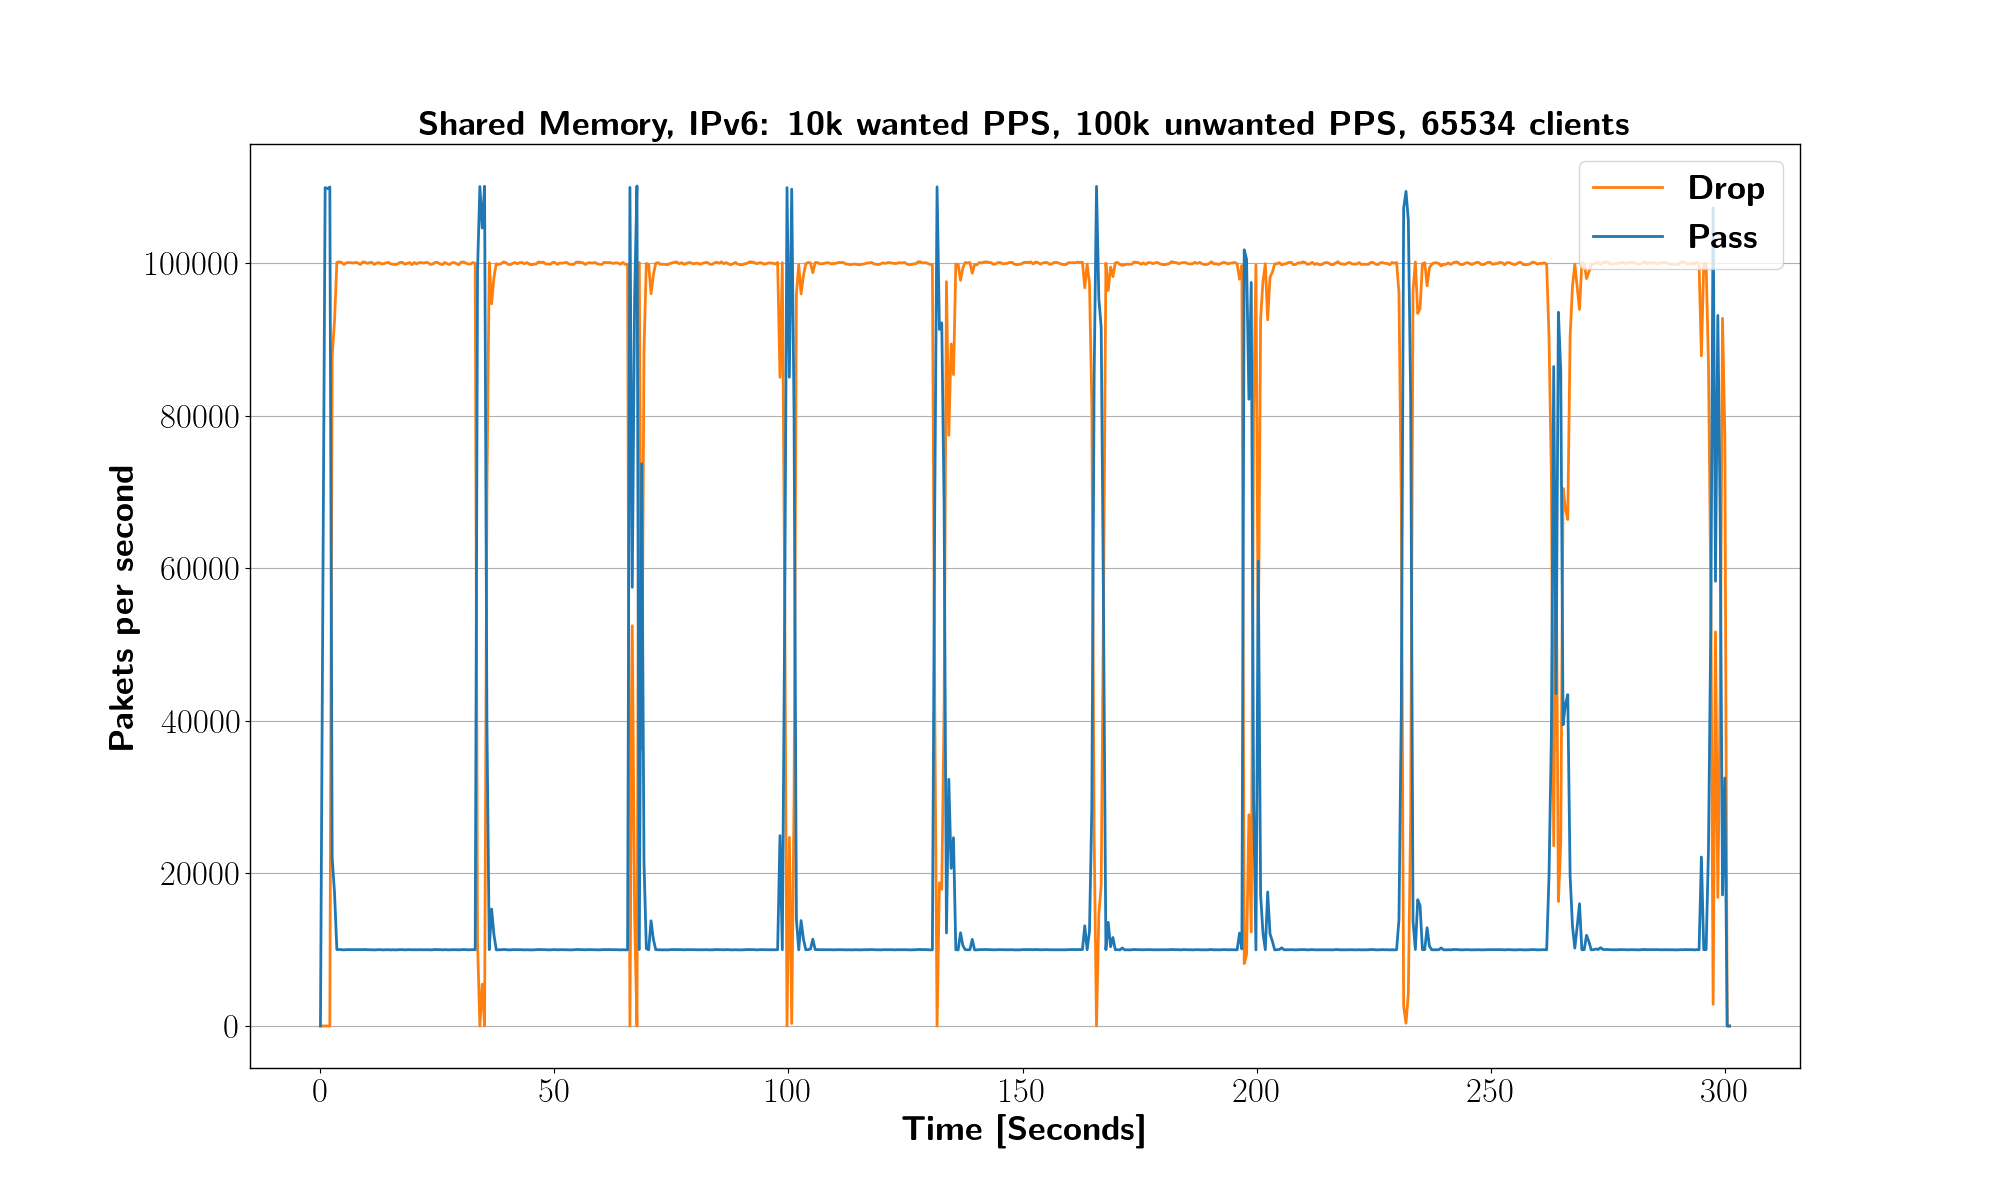
\includegraphics[width=1.2\textwidth]{images/simplefail2ban_shm_ipv6_v10k_iv100k_c65534.png}}
	\end{tabular}
	\begin{tabular}{lllll}
		\toprule
		\textbf{Total packets [$10^6$]} & \textbf{Packets dropped [$10^6$]} & \textbf{Relative drop [\%]} & \textbf{Log messages [$10^6$]} & \textbf{CPU [seconds]} \\ \midrule 
		33 & 27.95 & 99.67 & 2.05 & 15.55 \\
		\bottomrule
	\end{tabular}
	\caption[Simplefail2ban, Shared Memory, IPv6, 100k \ac{PPS}]{Some text}
\end{figure}

\begin{figure}[p]
	\label{fig:simplefail2ban:shm:ip6:1m}
	\centering
	\scriptsize
	\begin{tabular}{c}
    	\centerline{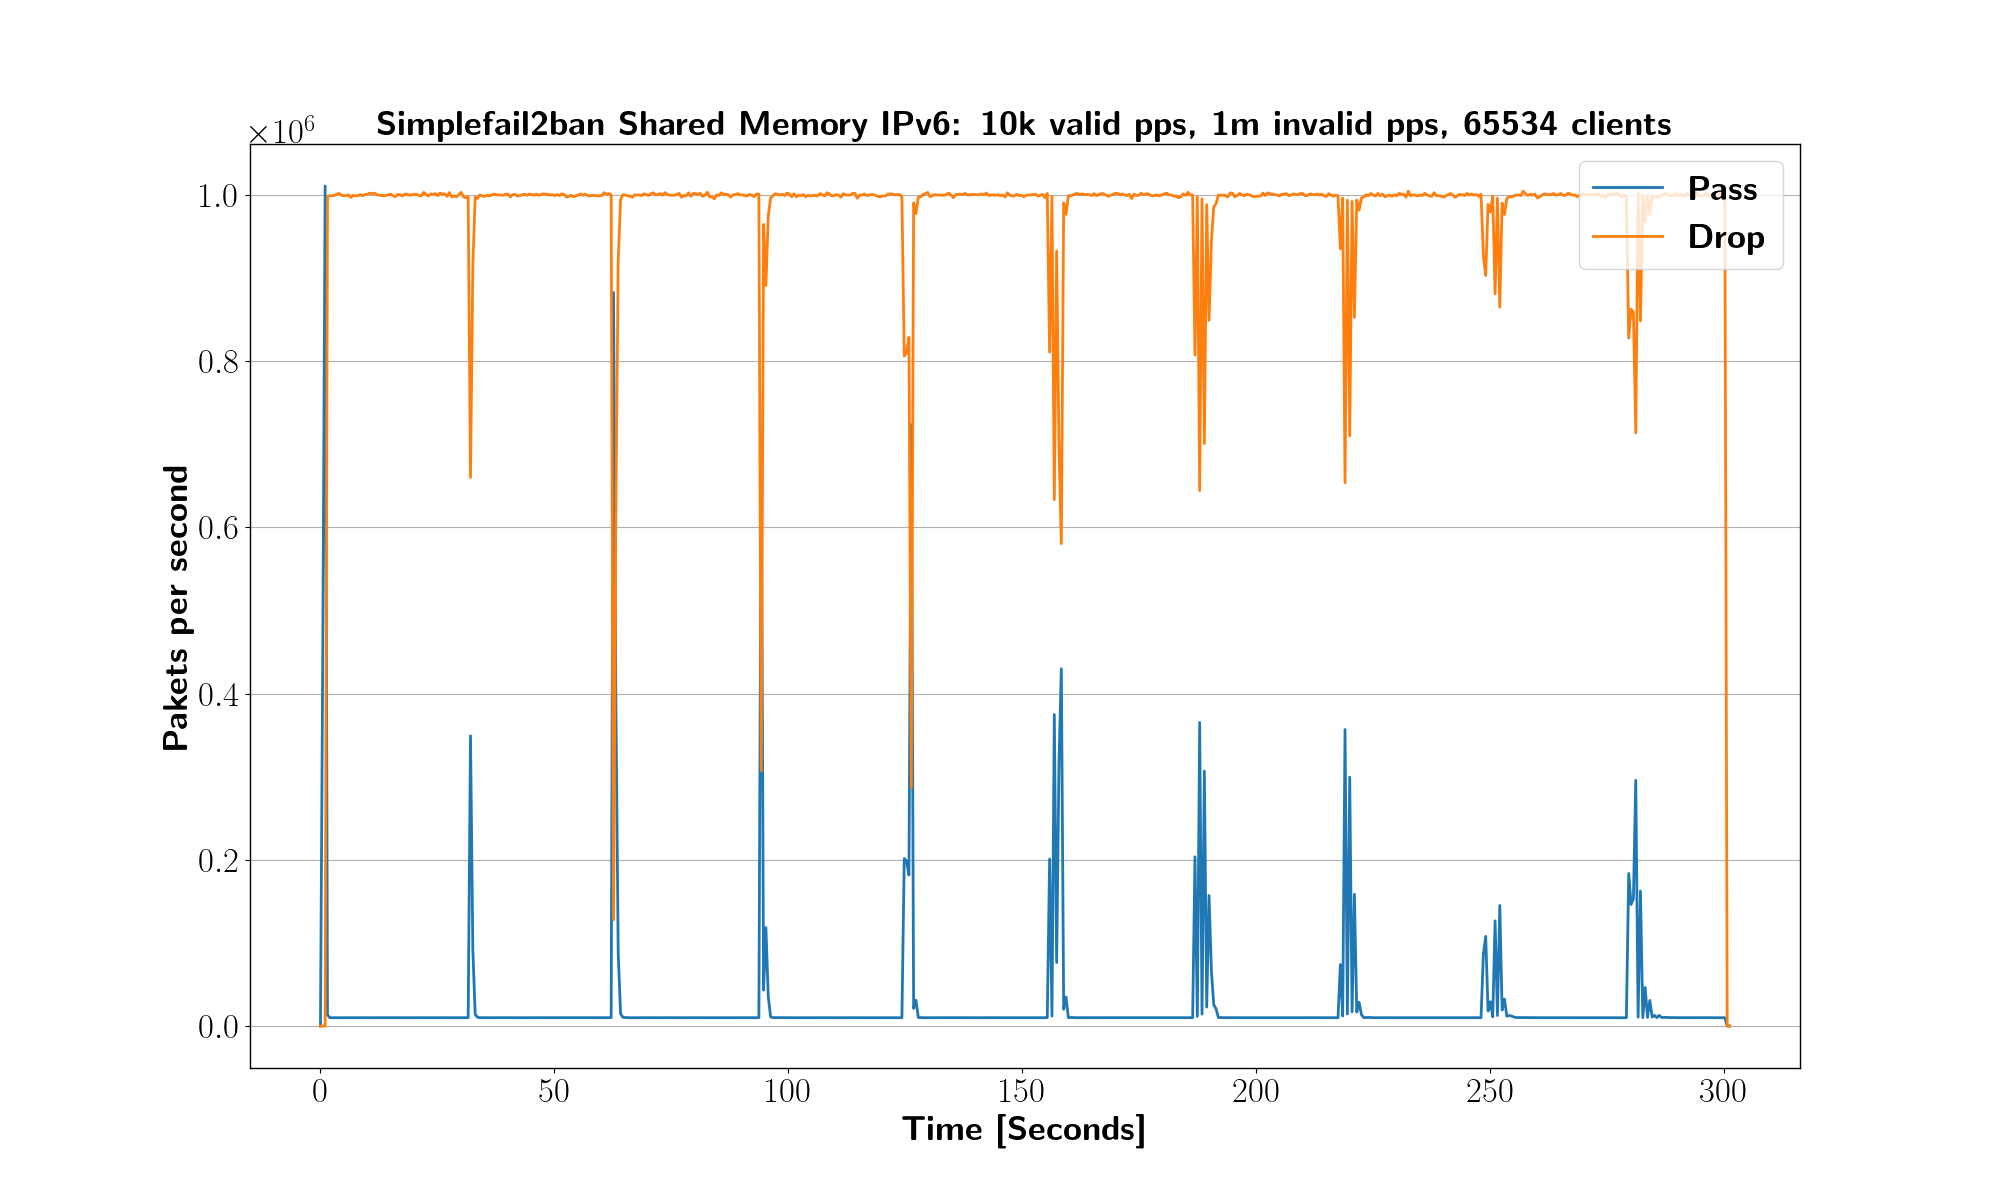
\includegraphics[width=1.2\textwidth]{images/simplefail2ban_shm_ipv6_v10k_iv1m_c65534.png}}
	\end{tabular}
	\begin{tabular}{lllll}
		\toprule
		\textbf{Total packets [$10^6$]} & \textbf{Packets dropped [$10^6$]} & \textbf{Relative drop [\%]} & \textbf{Log messages [$10^6$]} & \textbf{CPU [seconds]} \\ \midrule 
		303 & 294.77 & 98.9 & 4.39 & 17.46 \\
		\bottomrule
	\end{tabular}
	\caption[Simplefail2ban, Shared Memory, IPv6, 1m \ac{PPS}]{Some text}
\end{figure}

\begin{figure}[p]
	\label{fig:simplefail2ban:shm:ip6:10m}
	\centering
	\scriptsize
	\begin{tabular}{c}
    	\centerline{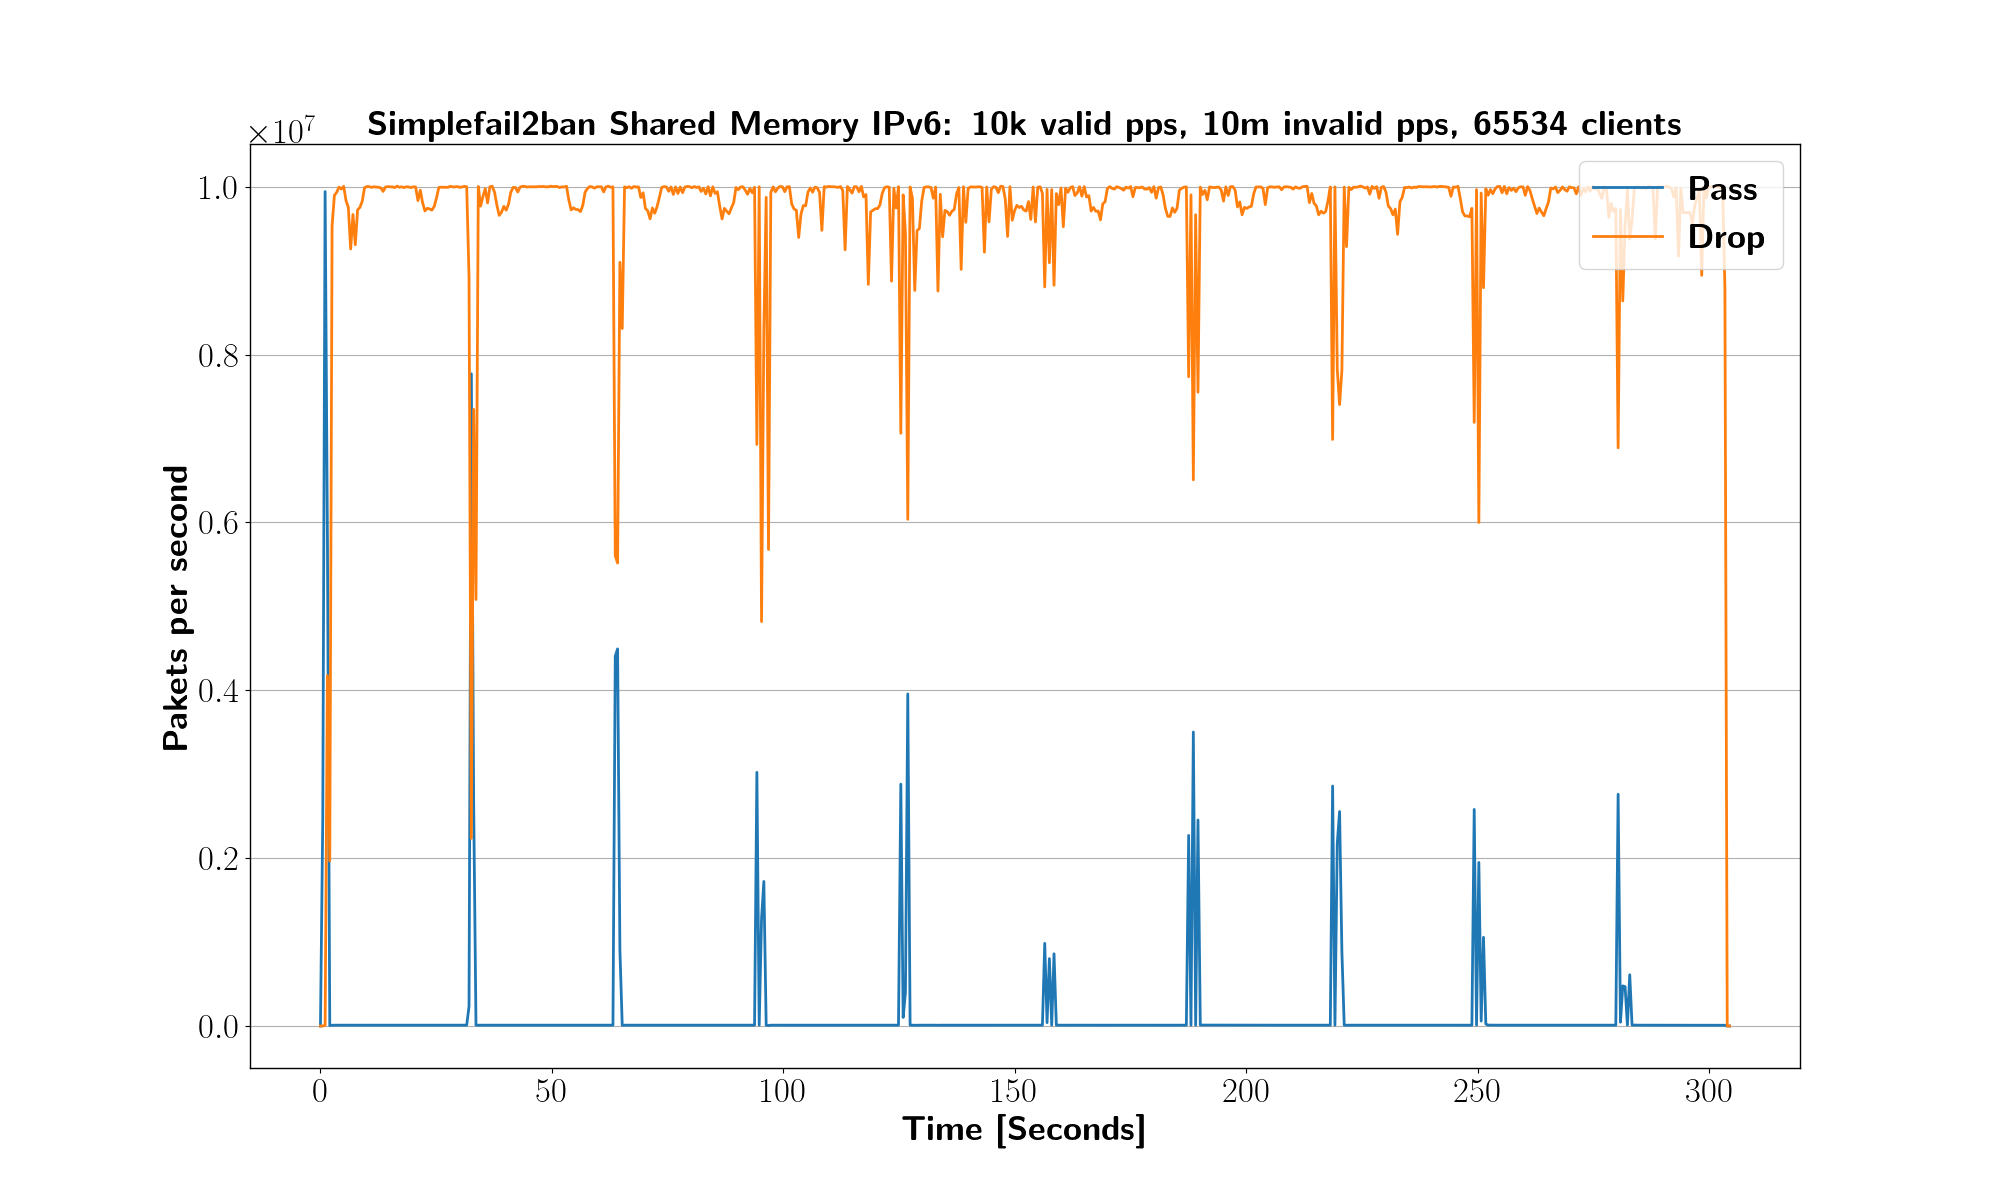
\includegraphics[width=1.2\textwidth]{images/simplefail2ban_shm_ipv6_v10k_iv10m_c65534.png}}
	\end{tabular}
	\begin{tabular}{lllll}
		\toprule
		\textbf{Total packets [$10^6$]} & \textbf{Packets dropped [$10^6$]} & \textbf{Relative drop [\%]} & \textbf{Log messages [$10^6$]} & \textbf{CPU [seconds]} \\ \midrule 
		2991.93 & 2947.1 & 98.66 & 8.88 & 32.36 \\
		\bottomrule
	\end{tabular}
	\caption[Simplefail2ban, Shared Memory, IPv6, 10m \ac{PPS}]{Some text}
\end{figure}

\begin{figure}[p]
	\label{fig:simplefail2ban:shm:ip46:100k}
	\centering
	\scriptsize
	\begin{tabular}{c}
    	\centerline{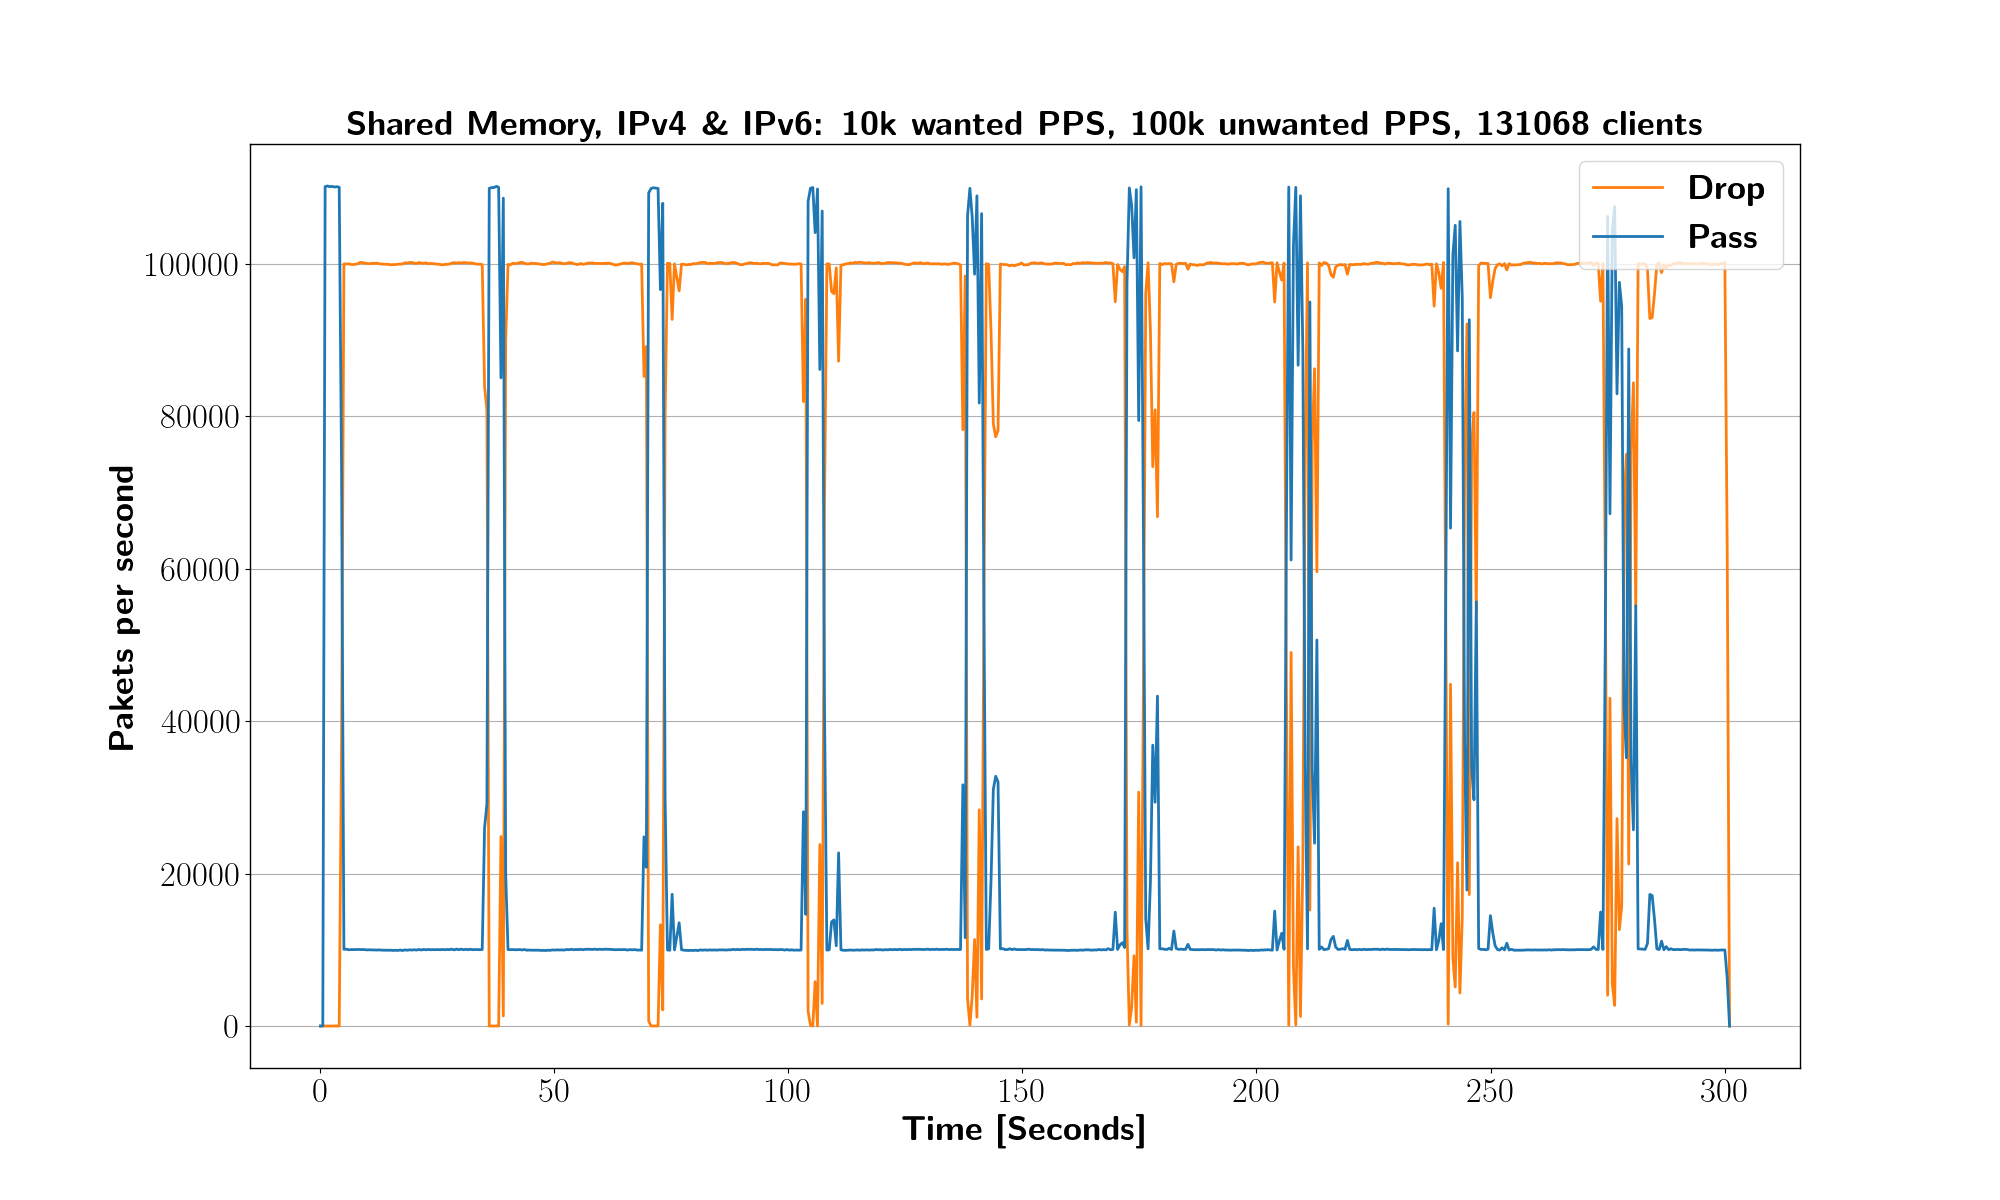
\includegraphics[width=1.2\textwidth]{images/simplefail2ban_shm_ipv46_v10k_iv100k_c131068.png}}
	\end{tabular}
	\begin{tabular}{lllll}
		\toprule
		\textbf{Total packets [$10^6$]} & \textbf{Packets dropped [$10^6$]} & \textbf{Relative drop [\%]} & \textbf{Log messages [$10^6$]} & \textbf{CPU [seconds]} \\ \midrule 
		33 & 26.45 & 99.95 & 3.55 & 26.35 \\
		\bottomrule
	\end{tabular}
	\caption[Simplefail2ban, Shared Memory, IPv4 \& IPv6, 100k \ac{PPS}]{Some text}
\end{figure}

\begin{figure}[p]
	\label{fig:simplefail2ban:shm:ip46:1m}
	\centering
	\scriptsize
	\begin{tabular}{c}
    	\centerline{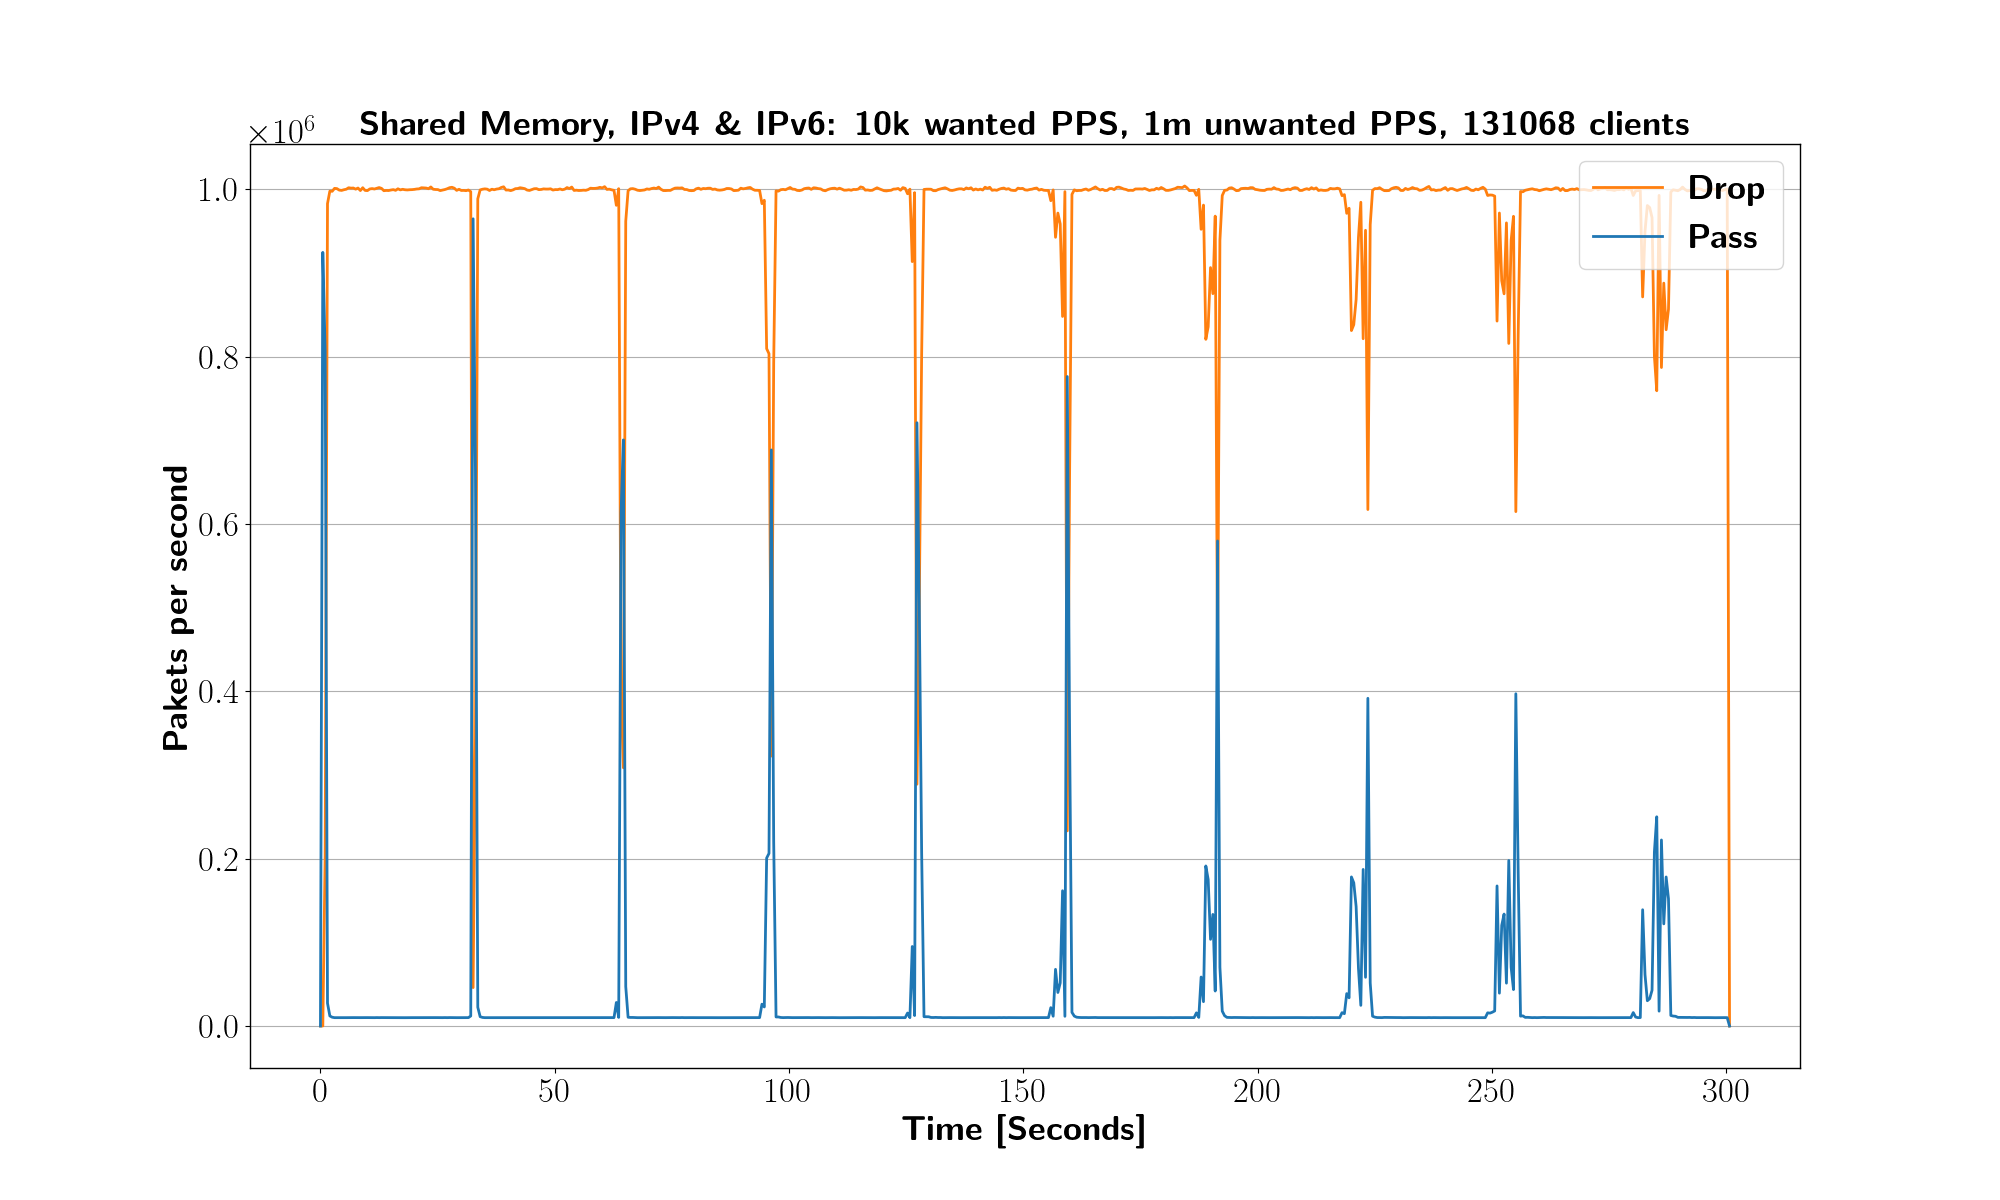
\includegraphics[width=1.2\textwidth]{images/simplefail2ban_shm_ipv46_v10k_iv1m_c131068.png}}
	\end{tabular}
	\begin{tabular}{lllll}
		\toprule
		\textbf{Total packets [$10^6$]} & \textbf{Packets dropped [$10^6$]} & \textbf{Relative drop [\%]} & \textbf{Log messages [$10^6$]} & \textbf{CPU [seconds]} \\ \midrule 
		303 & 293.13 & 99 & 5.95 & 27.66 \\
		\bottomrule
	\end{tabular}
	\caption[Simplefail2ban, Shared Memory, IPv4 \& IPv6, 1m \ac{PPS}]{Some text}
\end{figure}

\begin{figure}[p]
	\label{fig:simplefail2ban:shm:ip46:10m}
	\centering
	\scriptsize
	\begin{tabular}{c}
    	\centerline{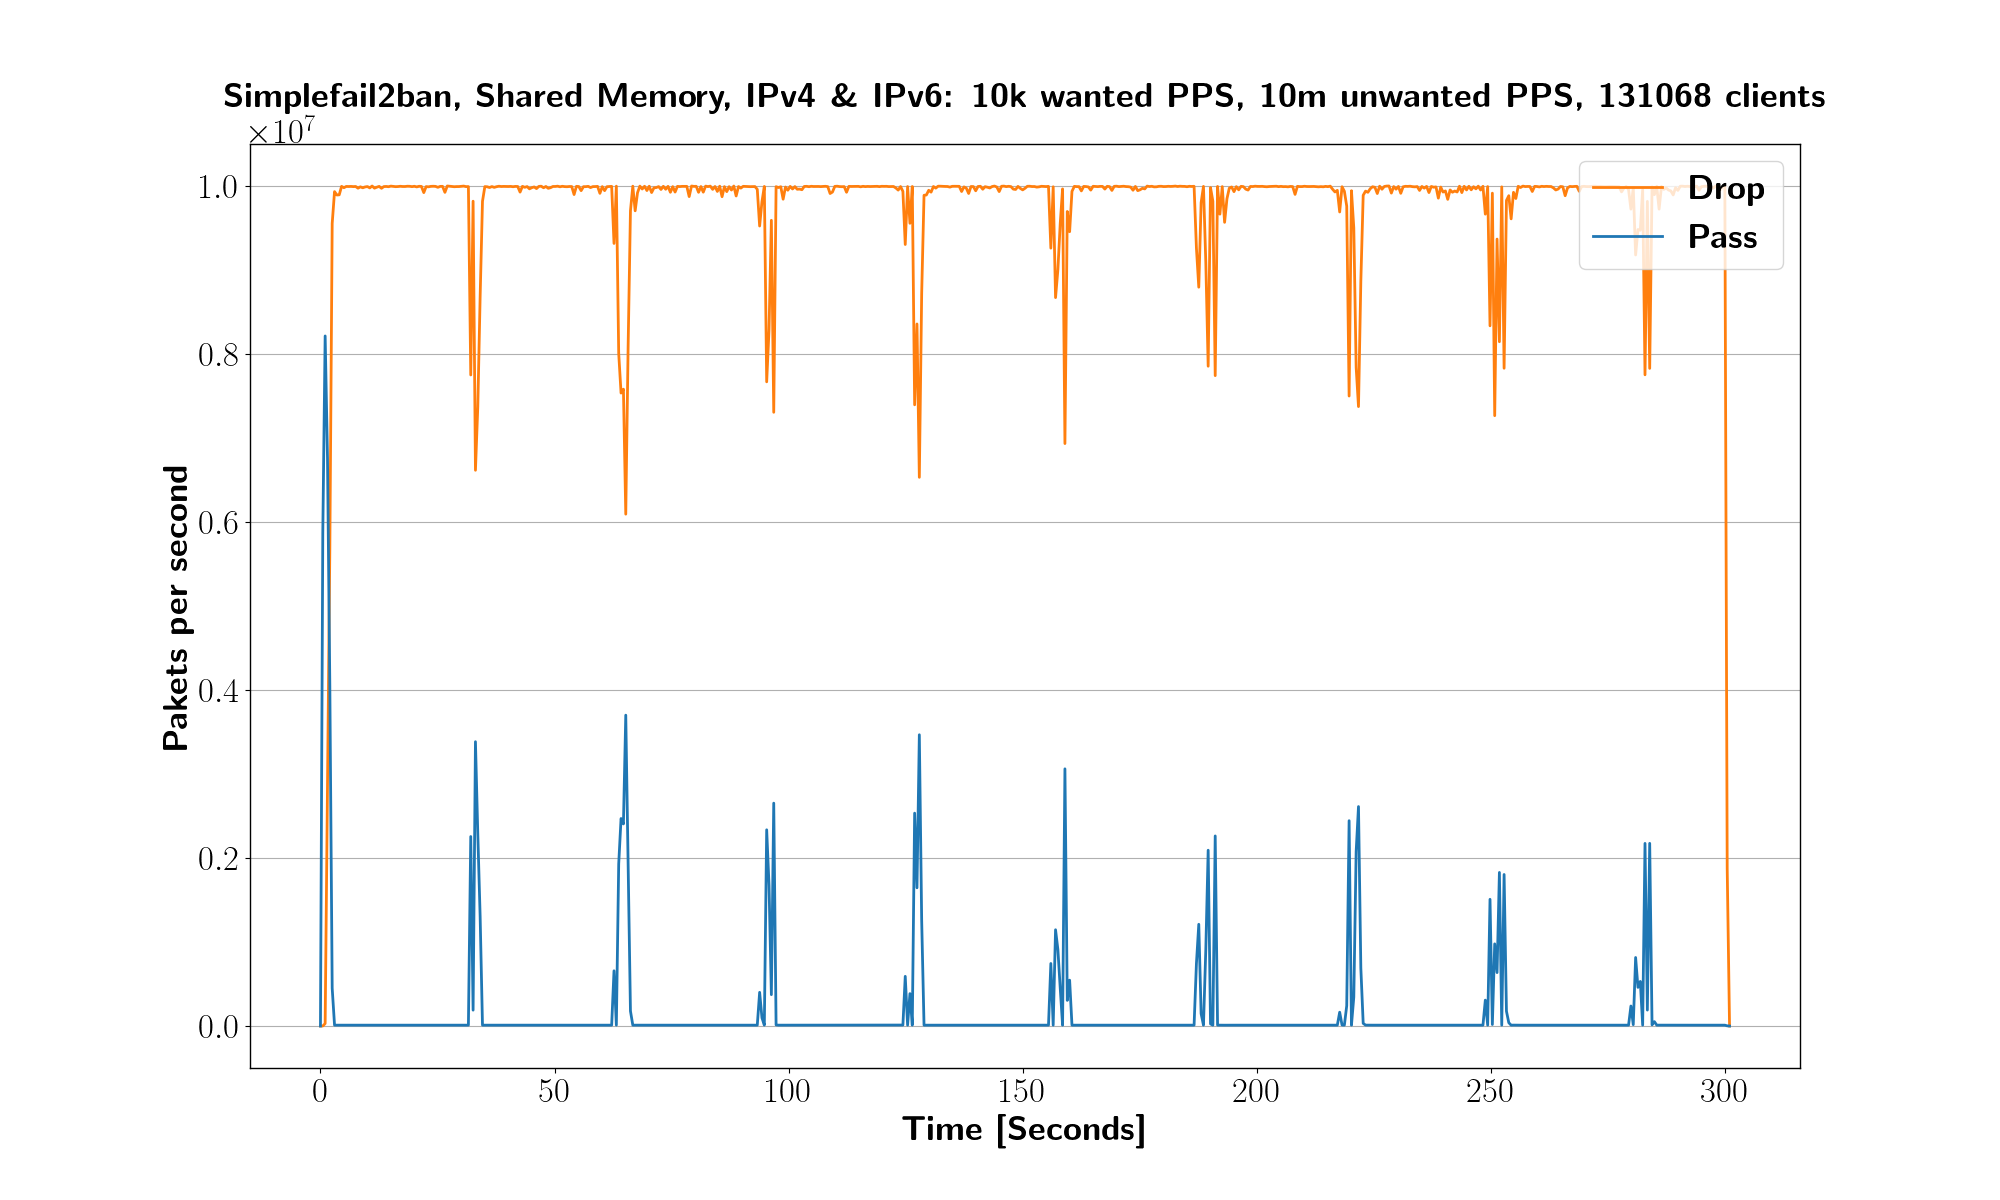
\includegraphics[width=1.2\textwidth]{images/simplefail2ban_shm_ipv46_v10k_iv10m_c131068.png}}
	\end{tabular}
	\begin{tabular}{lllll}
		\toprule
		\textbf{Total packets [$10^6$]} & \textbf{Packets dropped [$10^6$]} & \textbf{Relative drop [\%]} & \textbf{Log messages [$10^6$]} & \textbf{CPU [seconds]} \\ \midrule 
		2992.44 & 2939.27 & 98.45 & 16.18 & 65.74 \\
		\bottomrule
	\end{tabular}
	\caption[Simplefail2ban, Shared Memory, IPv4 \& IPv6, 10m \ac{PPS}]{Some text}
\end{figure}

\section{Shared Memory Special Measurements}

\begin{figure}[p]
	\label{fig:simplefail2ban:shm:2r}
	\centering
	\scriptsize
	\begin{tabular}{c}
    	\centerline{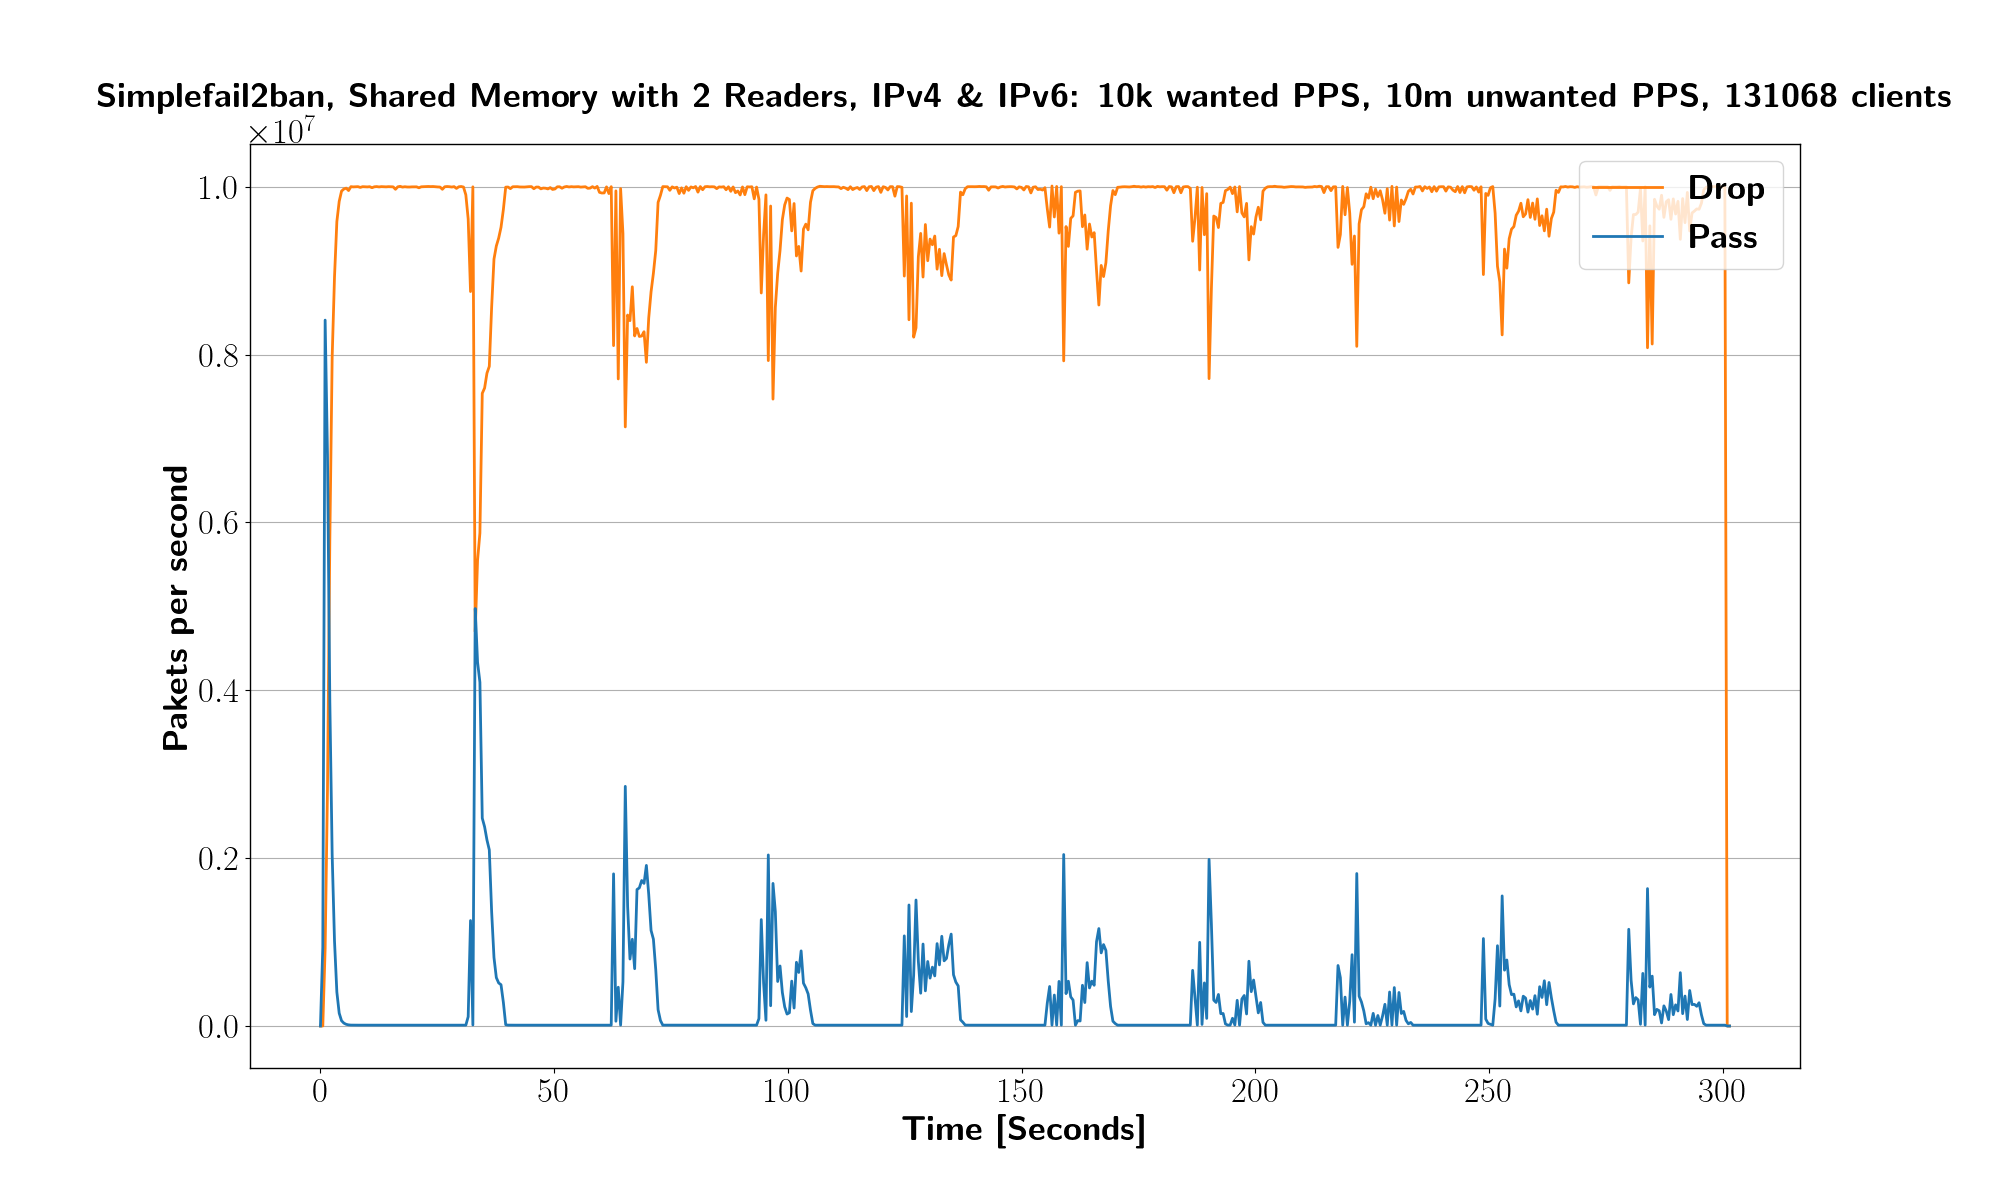
\includegraphics[width=1.2\textwidth]{images/simplefail2ban_shm_2r_ipv46_v10k_iv10m_c131068.png}}
	\end{tabular}
	\begin{tabular}{lllll}
		\toprule
		\textbf{Total packets [$10^6$]} & \textbf{Packets dropped [$10^6$]} & \textbf{Relative drop [\%]} & \textbf{Log messages [$10^6$]} & \textbf{CPU [seconds]} \\ \midrule 
		2989.66 & 2906.36 & 97.44 & 17.67 & 77.19 \\
		\bottomrule
	\end{tabular}
	\caption[Simplefail2ban, Shared Memory 2 Readers]{Some text}
\end{figure}

\begin{figure}[p]
	\label{fig:simplefail2ban:shm:or}
	\centering
	\scriptsize
	\begin{tabular}{c}
    	\centerline{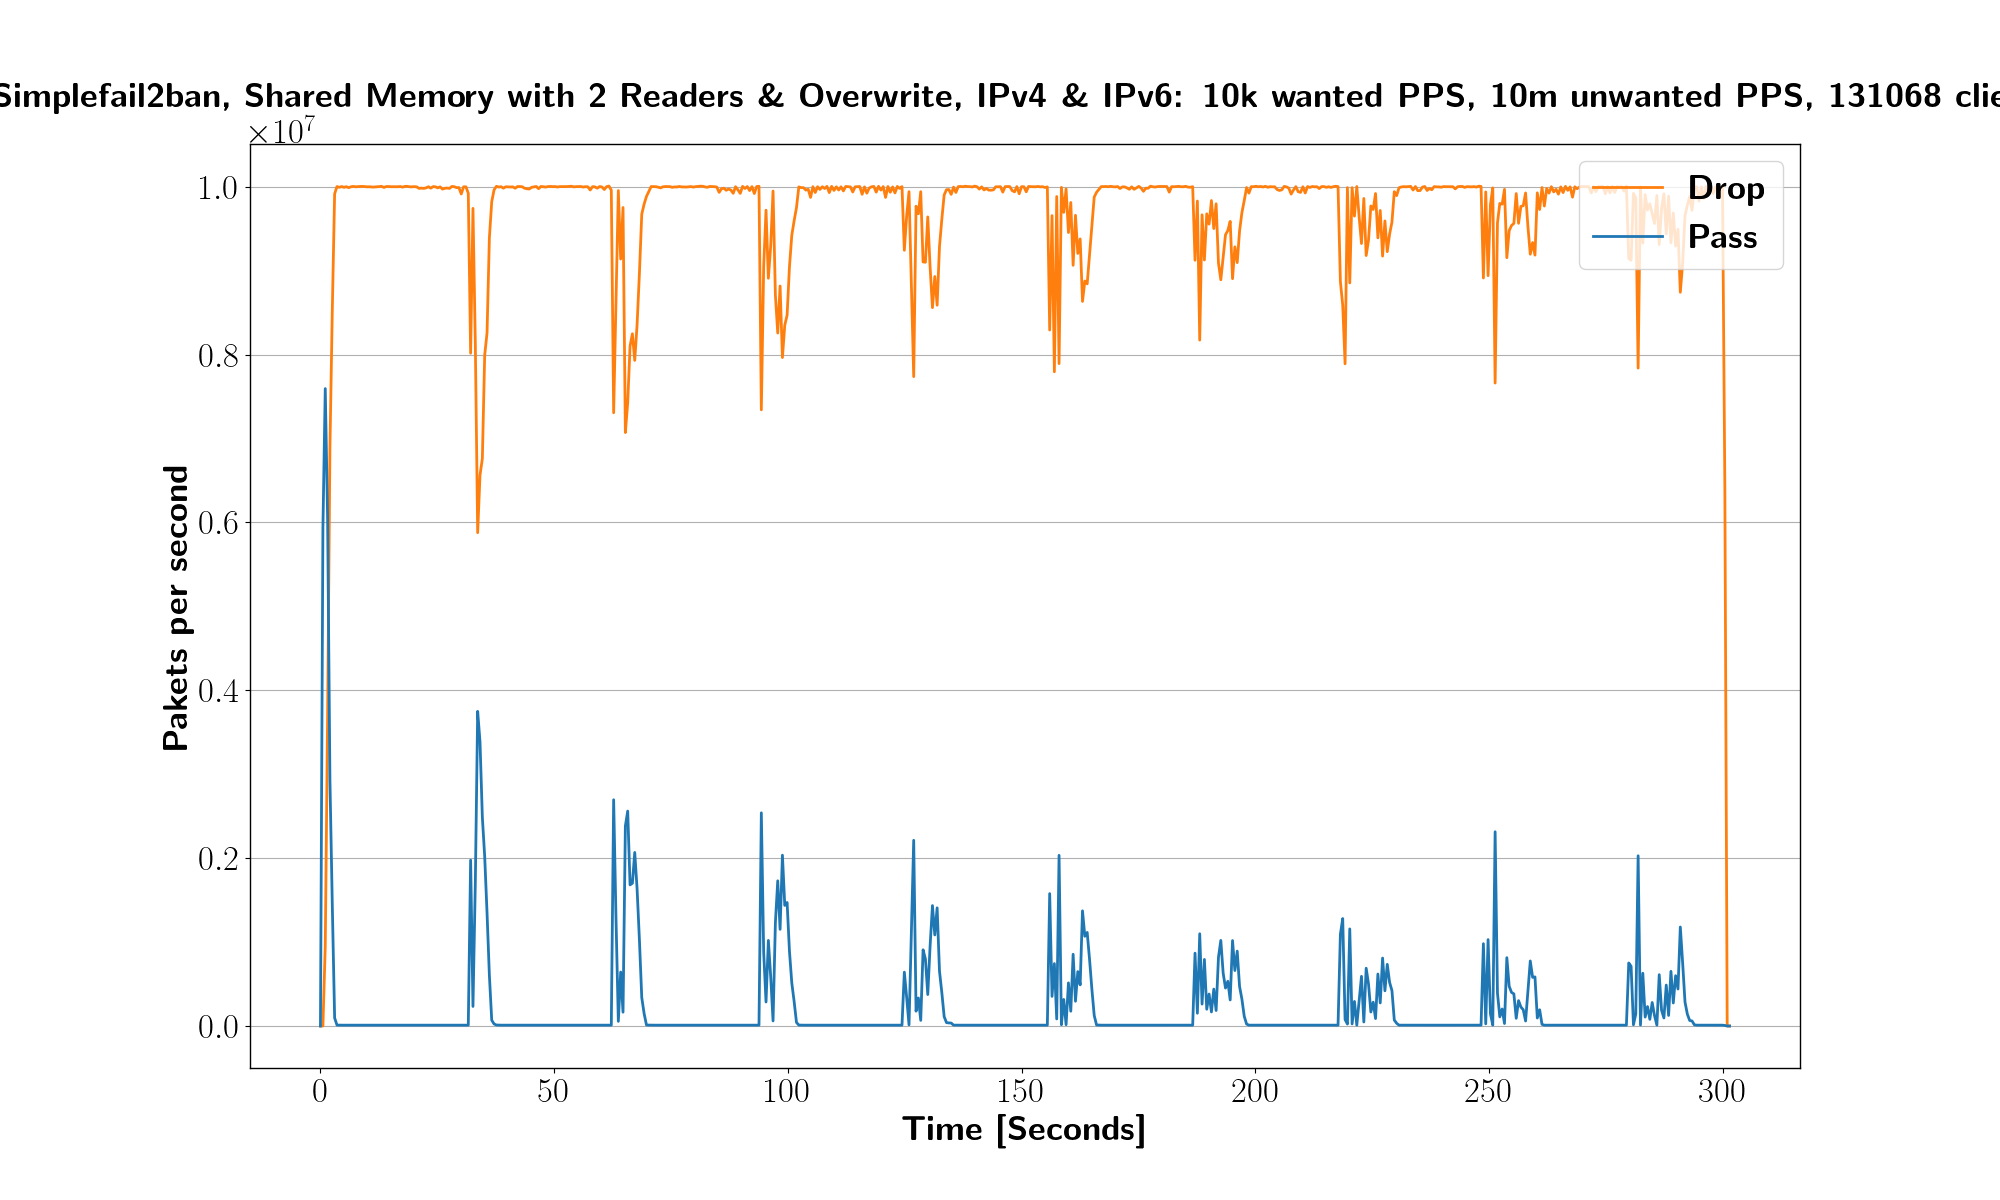
\includegraphics[width=1.2\textwidth]{images/simplefail2ban_shm_2r_or_ipv46_v10k_iv10m_c131068.png}}
	\end{tabular}
	\begin{tabular}{lllll}
		\toprule
		\textbf{Total packets [$10^6$]} & \textbf{Packets dropped [$10^6$]} & \textbf{Relative drop [\%]} & \textbf{Log messages [$10^6$]} & \textbf{CPU [seconds]} \\ \midrule 
		2988.9 & 2914.39 & 97.73 & 17.66 & 79.13 \\
		\bottomrule
	\end{tabular}
	\caption[Simplefail2ban, Shared Memory 2 Readers with Overwrite]{Some text}
\end{figure}

\begin{figure}[p]
	\label{fig:simplefail2ban:shm:ws}
	\centering
	\scriptsize
	\begin{tabular}{c}
    	\centerline{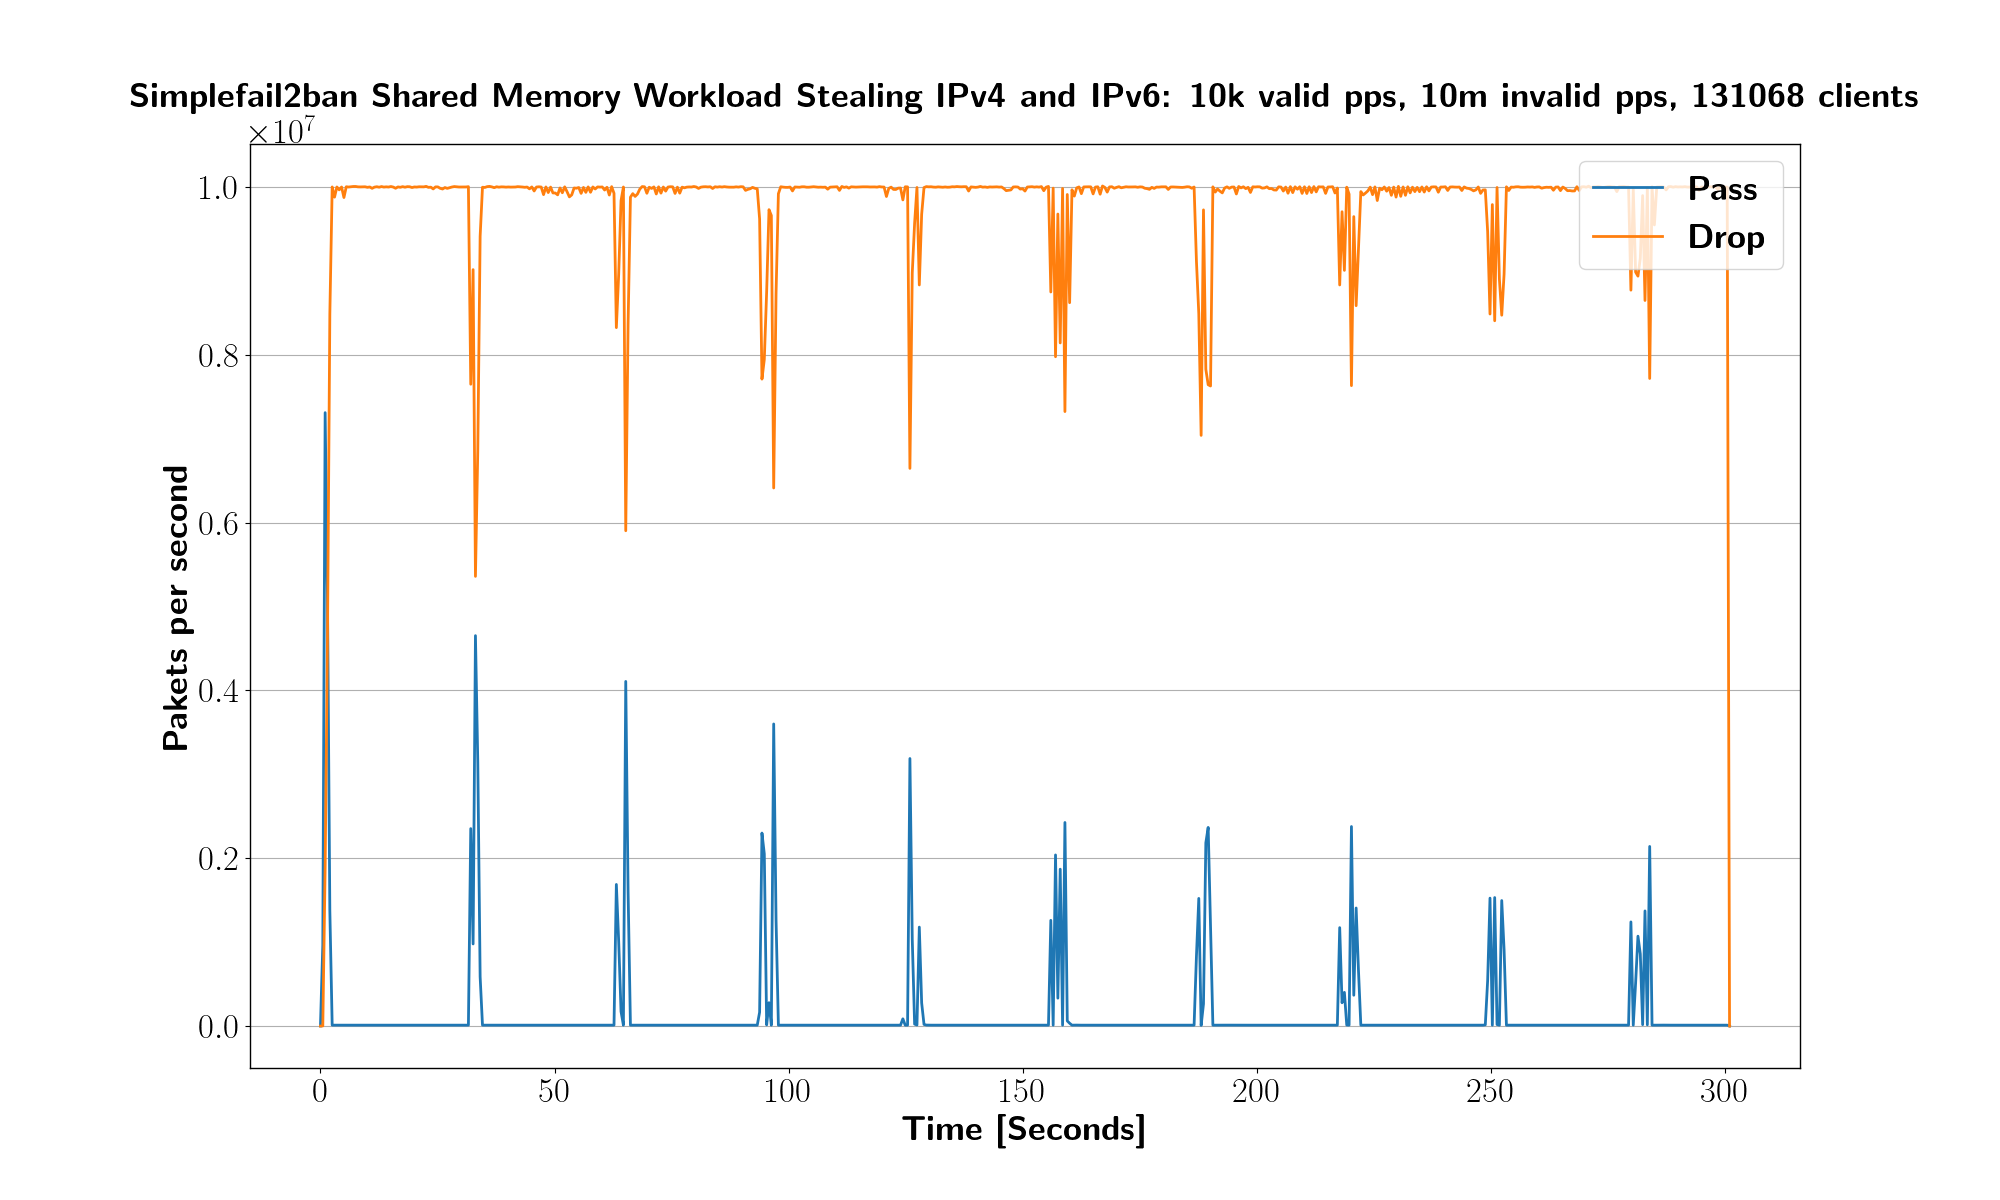
\includegraphics[width=1.2\textwidth]{images/simplefail2ban_shm_ws_ipv46_v10k_iv10m_c131068.png}}
	\end{tabular}
	\begin{tabular}{lllll}
		\toprule
		\textbf{Total packets [$10^6$]} & \textbf{Packets dropped [$10^6$]} & \textbf{Relative drop [\%]} & \textbf{Log messages [$10^6$]} & \textbf{CPU [seconds]} \\ \midrule 
		2991.23 & 2944.56 & 98.67 & 15.28 & 61 \\
		\bottomrule
	\end{tabular}
	\caption[Simplefail2ban, Shared Memory with Workload Sharing]{Some text}
\end{figure}

\begin{figure}[p]
	\label{fig:simplefail2ban:shm:nr}
	\centering
	\scriptsize
	\begin{tabular}{c}
    	\centerline{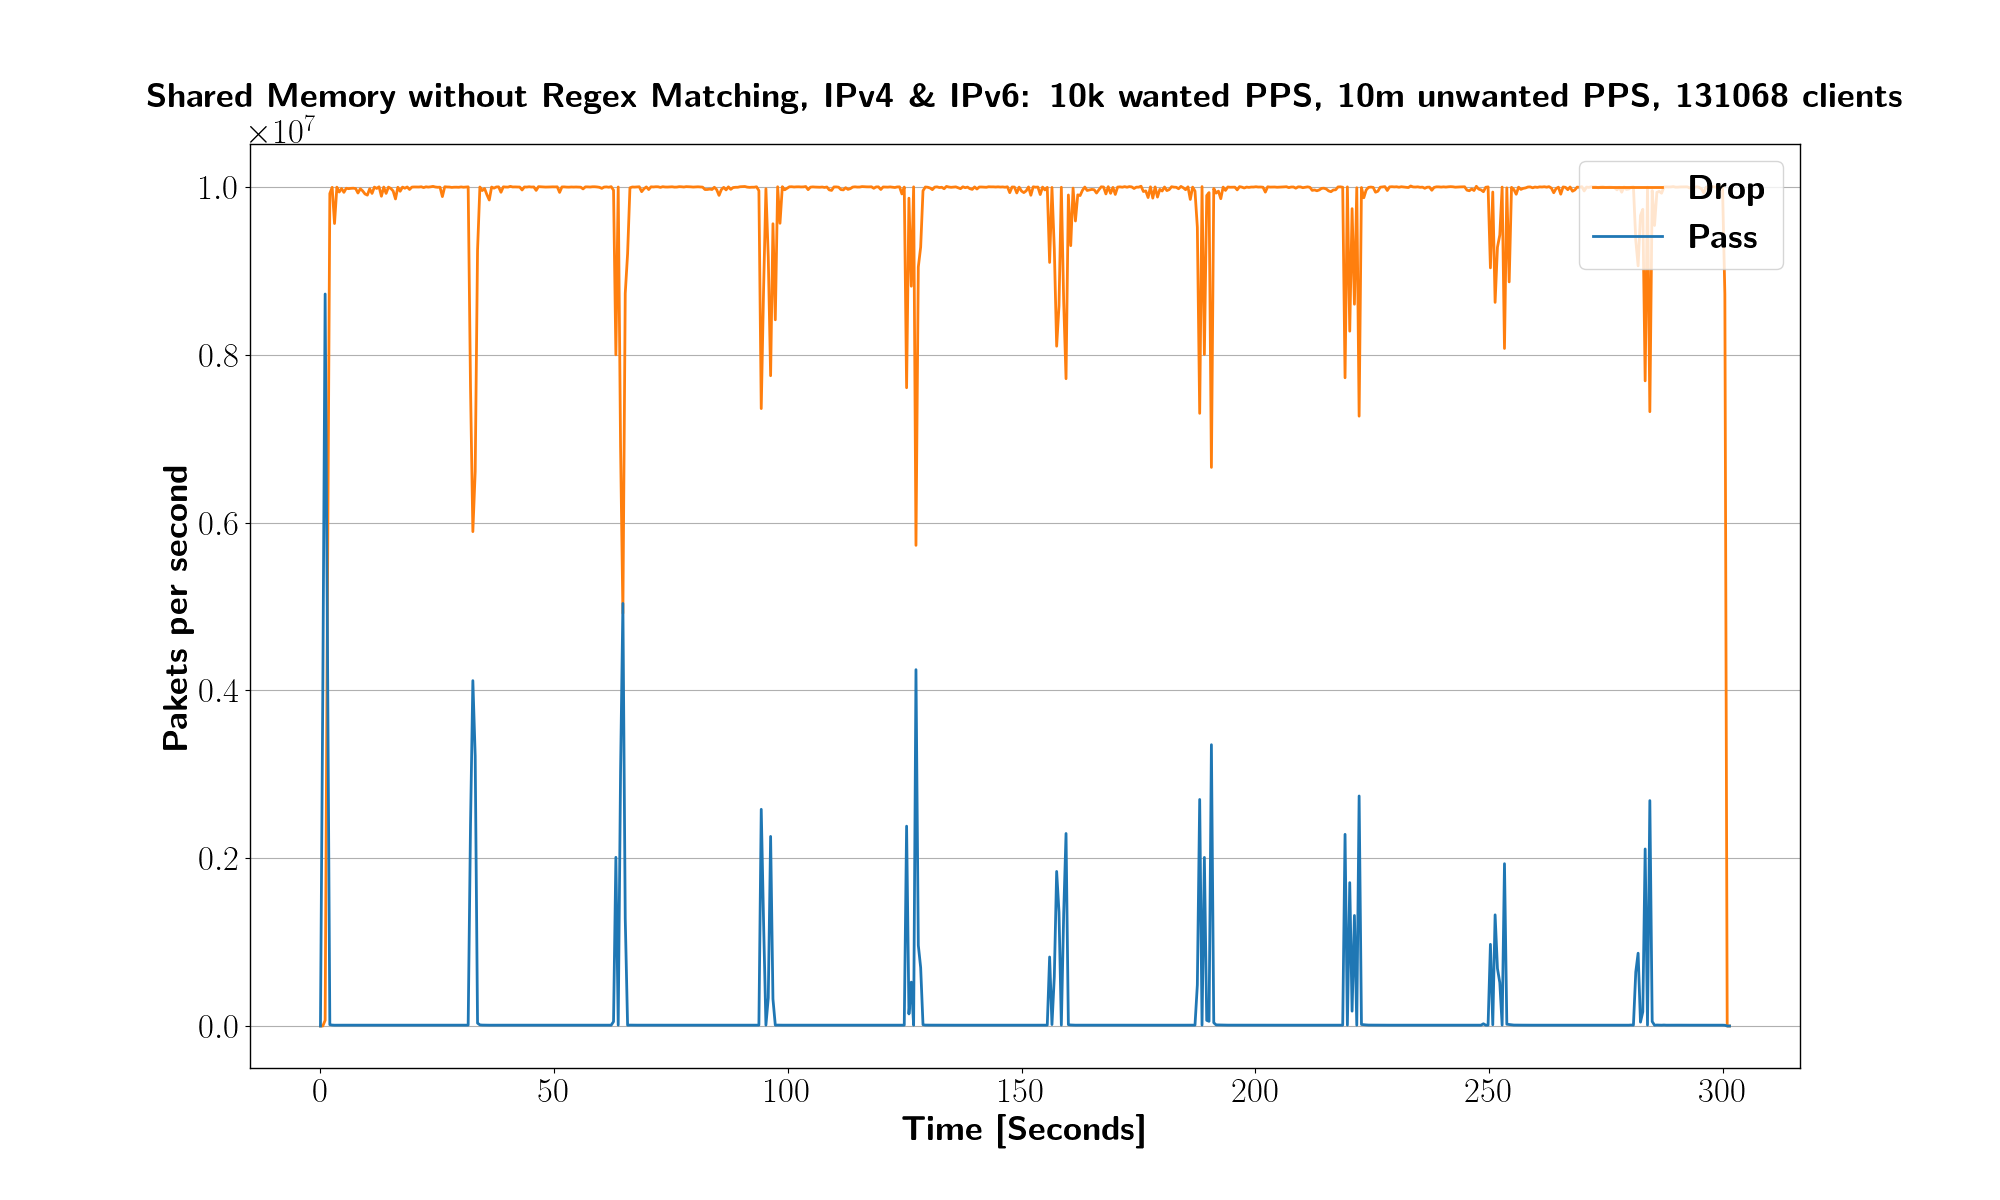
\includegraphics[width=1.2\textwidth]{images/simplefail2ban_shm_nr_ipv46_v10k_iv10m_c131068.png}}
	\end{tabular}
	\begin{tabular}{lllll}
		\toprule
		\textbf{Total packets [$10^6$]} & \textbf{Packets dropped [$10^6$]} & \textbf{Relative drop [\%]} & \textbf{Log messages [$10^6$]} & \textbf{CPU [seconds]} \\ \midrule 
		2989.56 & 2941.9 & 98.63 & 13.29 & 34.04 \\
		\bottomrule
	\end{tabular}
	\caption[Simplefail2ban, Shared Memory without Regex Matching]{Some text}
\end{figure}

\begin{figure}[p]
	\label{fig:simplefail2ban:shm:ip46:30m}
	\centering
	\scriptsize
	\begin{tabular}{c}
    	\centerline{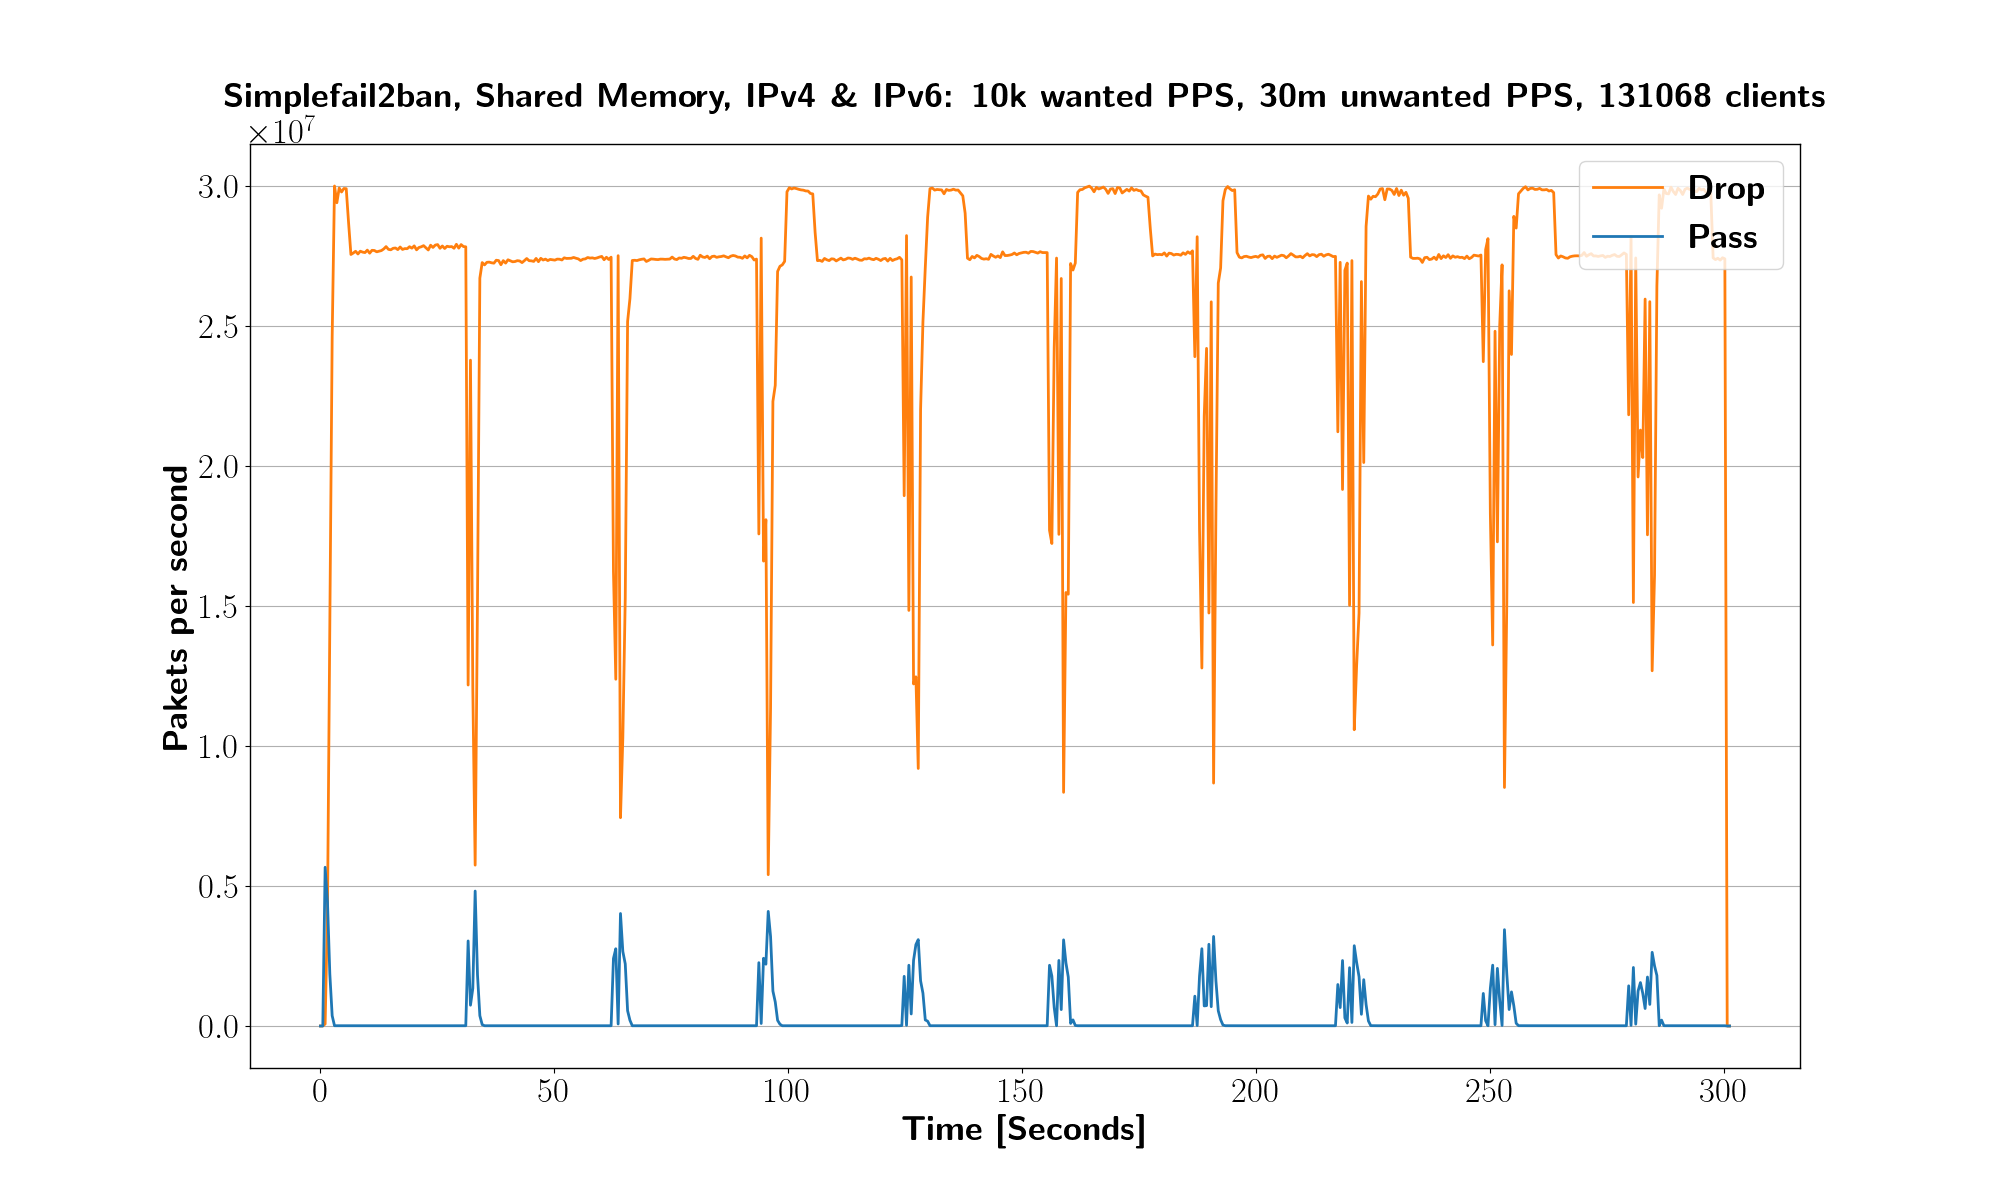
\includegraphics[width=1.2\textwidth]{images/simplefail2ban_shm_ipv46_v10k_iv30m_c131068.png}}
	\end{tabular}
	\begin{tabular}{lllll}
		\toprule
		\textbf{Total packets [$10^6$]} & \textbf{Packets dropped [$10^6$]} & \textbf{Relative drop [\%]} & \textbf{Log messages [$10^6$]} & \textbf{CPU [seconds]} \\ \midrule 
		8095.28 & 8017.72 & 99.13 & 21 & 76.23 \\
		\bottomrule
	\end{tabular}
	\caption[Simplefail2ban, Shared Memory, IPv4 \& IPv6, 30m \ac{PPS}]{Some text}
\end{figure}

% reset acronym counter
%%acresetall
% include a chapter
%
% $Id: chapter6.tex 2628 2008-06-04 11:21:59Z jozinke $
%
%%\pagestyle{scrheadings}
%%\ohead[]{}
%%\ihead[]{}
%%\chead[]{}
%%\ofoot[\pagemark]{\pagemark}
%%\ifoot[]{}
\chapter{Conclusion}

% reset acronym counter 
%%%acresetall 
% include a chapter 
%\include{chapter7}
% reset acronym counter
%%%acresetall
% include a chapter
%\include{chapter8}
% include outro 
%
% $Id: outro.tex 2771 2008-10-15 16:29:47Z sliske $
%
\addtocontents{toc}{\protect\newpage}
% start the appendix (changes section numbering, and others)
\appendix
% use different page style
\pagestyle{appendixstyle}
%reset acronym counter
% \acresetall % really? (by stefan)

%list of figures
%

\listoffigures
%\cleardoublepage

%
% list of tables
%

\listoftables
%\cleardoublepage

%
% list of algorithms
%

\listofalgorithms
%\cleardoublepage

%
% list of abbreviations
%

\iflanguage{ngerman}
{
\chapter{Abkürzungsverzeichnis}
}{
\chapter{Abbreviations}
}
\begin{acronym}[skbufflonglon]
\acro{API}{Application Programming Interface}
\acro{AMQP}{Advanced Message Queue Protocol}
\acro{ARM}{Advanced \acs{RISC} Machines}
\acro{BCC}{BPF Compiler Collection}
\acro{BIND}{Berkeley Internet Name Domain Server}
 \acro{BPF}{Berkeley Packet Filter}
 \acro{BPF CORE}{BPF Compile Once Run Everywhere}
 \acro{BTF}{BPF Type Format}
 \acro{cBPF}{classical Berkeley Packet Filter}
 \acro{CPU}{Central Processing Unit}
 \acro{DNS}{Domain Name System}
 \acro{DUT}{Device under Test}
 \acro{DDIO}{Direct Data Input Output}
 \acro{DoS}{Denial of Service}
 \acro{DDoS}{Distributed Denial of Service}
 \acro{DMA}{Direct Memory Access}
 \acro{DPDK}{Data Plane Development Kit}
 \acro{eBPF}{extended Berkeley Packet Filter}
 \acro{ESP}{Encapsulating Security Payload}
 \acro{FIFO}{First in First out}
 \acro{HIDS}{Host-based Intrusion Detection System}
 \acro{HTTP}{Hypertext Transfer Protocol}
 \acro{IANA}{Internet Assigned Numbers Authority}
 \acro{IDS}{Intrusion Detection System}
 \acro{IEEE}{Institute of Electrical and Electronics Engineers}
 \acro{IP}{Internet Protocol}
 \acro{IPC}{Inter-Process Communication}
 \acro{IPS}{Intrusion Prevention System}
 \acro{IPsec}{\acs{IP} Security}
 \acro{IPv4}{Internet Protocol Version 4}
 \acro{IPv6}{Internet Protocol Version 6}
 \acro{IO}{Input / Output}
 \acro{ISP}{Internet Service Provider}
 \acro{JIT}{Just in Time}
 \acro{LLVM}{Low Level Virtual Machine}
 \acro{MAC}{Media Control Access}
 \acro{MPPS}{Million Packets Per Second}
 \acro{MTU}{Maximum Transfer Unit}
 \acro{NAPI}{New \acs{API}}
 \acro{API}{Application Programming Interface}
 \acro{NAT}{Network Address Translation}
 \acro{NIC}{Network Interface Card}
 \acro{NIDS}{Network-based Intrusion Detection System}
 \acro{NSD}{Name Server Daemon}
 \acro{pcap}{Packet Capture}
 \acro{OS}{Operating System}
 \acro{OSI}{Open Systems Interconnection}
 \acro{PCI}{Peripheral Component Interconnect}
 \acro{PoC}{Proof of Concept}
 \acro{PPS}{Packets per Second}
 \acro{RAM}{Random Access Memory}
 \acro{regex}{regular expression}
 \acro{RIPE}{Réseaux IP Européens (European \ac{IP} Networks)}
 \acro{RISC}{Reduced Instruction Set Computer}
 \acro{RFC}{Request for Comments}
 \acro{Regex}{Regular Expression}
 \acro{skbuff}[\texttt{sk\textunderscore buff}]{Socket Buffer}
 \acro{SSH}{Secure Shell}
 \acro{SIEM}{Security Information and Event Management}
 \acro{tc}[\texttt{tc}]{Traffic Control}
 \acro{TCP}{Transmission Control Protocol}
 \acro{TLS}{Transport Layer Security}
 \acro{UDP}{User Datagram Protocol}
 \acro{VM}{Virtual Machine}
 \acro{VLAN}{Virtual Local Area Network}
 \acro{XDP}{eXpress Data Path}
 \acro{RAM}{Random Access Memory}

 \acrodefplural{OS}[OS's]{Operating Systems}
 \acrodefplural{IPS}[IPS]{Intrusion Detection Systems}
 \acrodefplural{HIDS}[HIDS]{Host-based Intrusion Detection Systems}
 \acrodefplural{NIDS}[NIDS]{Network-based Intrusion Detection Systems}
 \acrodefplural{API}[APIs]{Application Programming Interfaces}


\end{acronym}
%\begingroup
%\let\clearpage\relax
\chapter{Source Files}
For the sake of not having to chop down a forest to print this thesis, no full source files will be appended.
The source code is available in a git repository at: \href{https://gitup.uni-potsdam.de/raatschen/bachelorarbeit}{https://gitup.uni-potsdam.de/raatschen/bachelorarbeit}.
Access can be requested through me, or the second supervisor Max Schrötter.
%\endgroup

\chapter{Measurements}


\begin{figure}[h!p]
	
	\centering
	\scriptsize
	\begin{tabular}{c}
    	\centerline{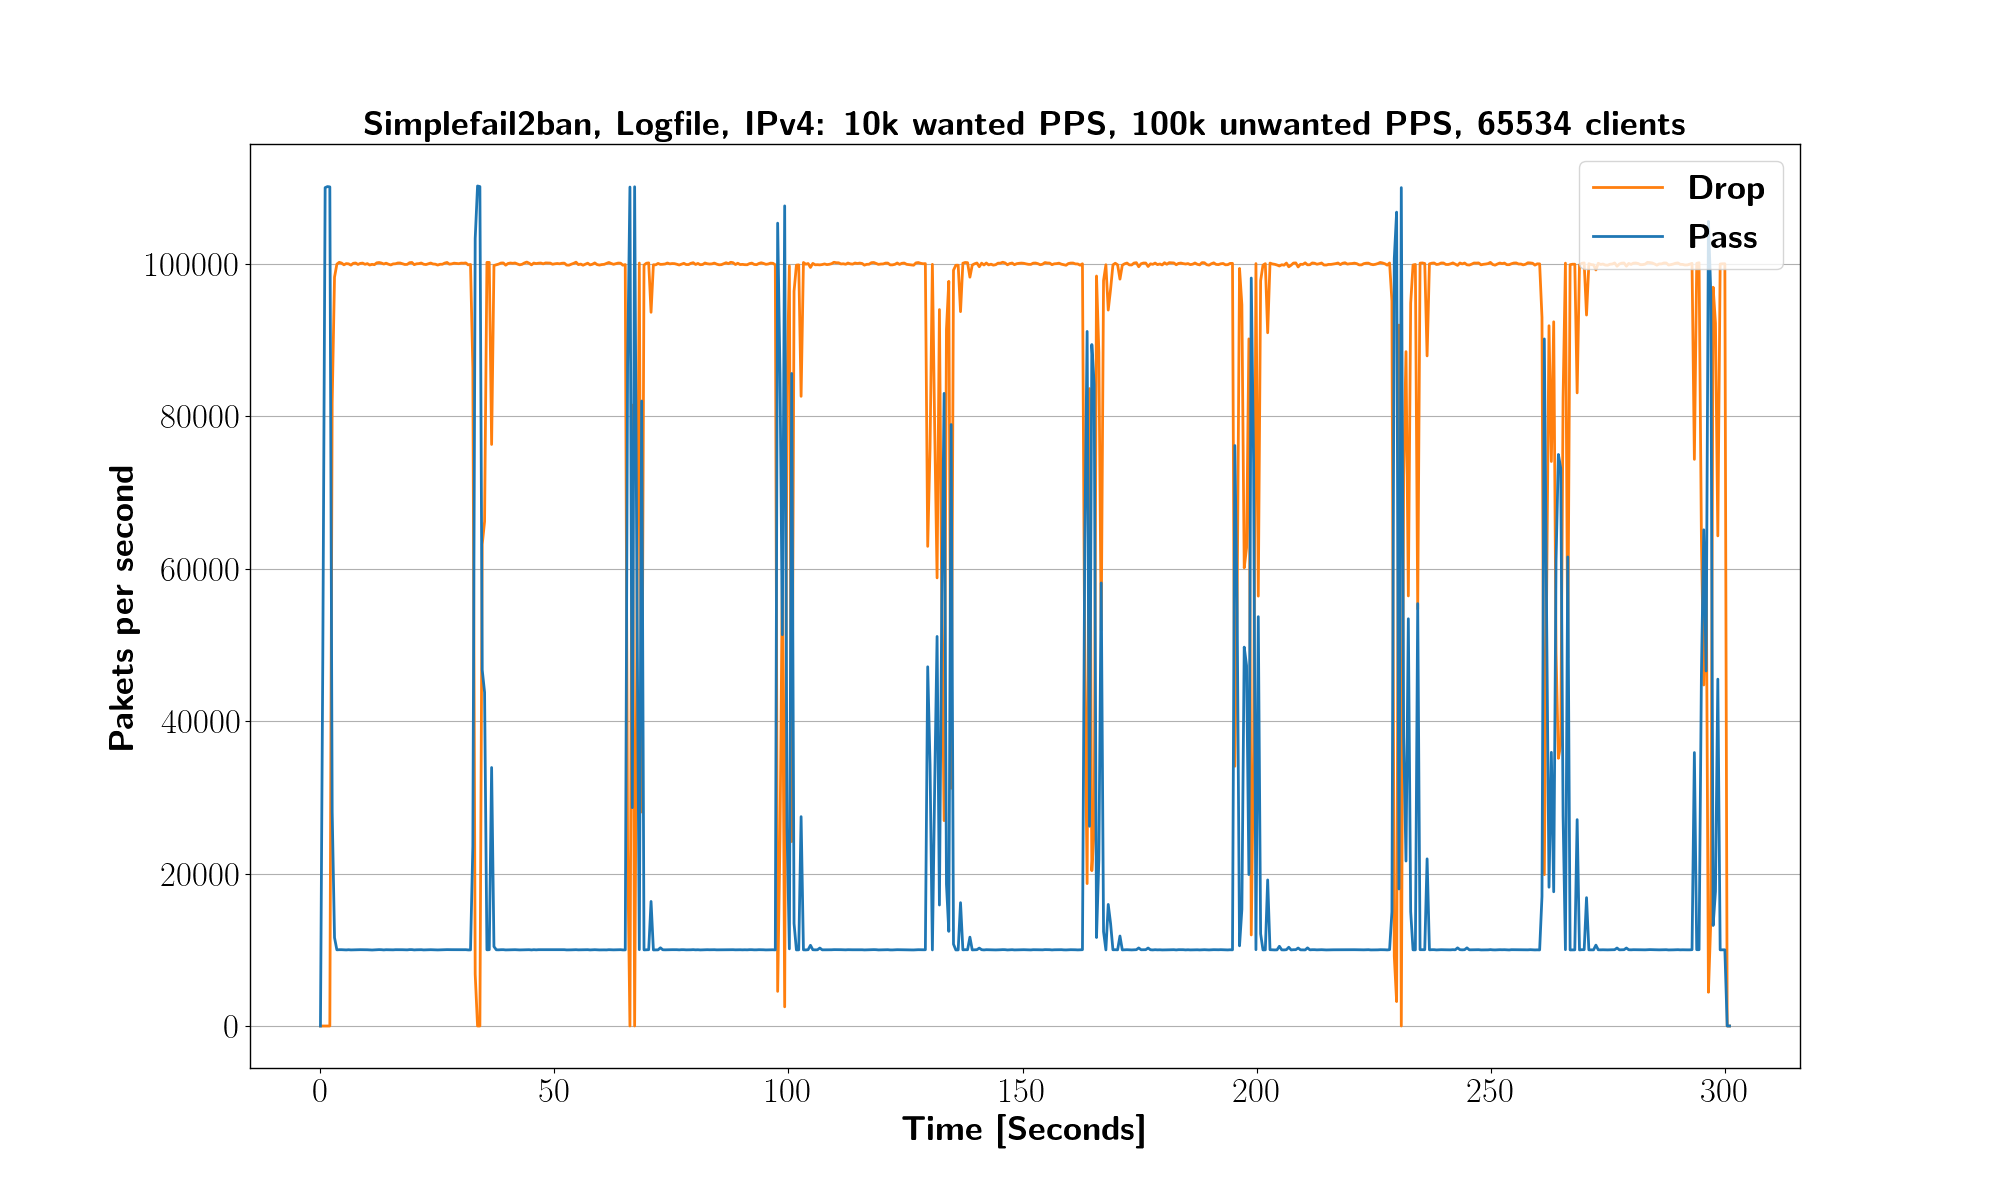
\includegraphics[width=1.2\textwidth]{images/simplefail2ban_disk_ipv4_v10k_iv100k_c65534.png}}
	\end{tabular}
	\begin{tabular}{lllll}
		\toprule
		\textbf{Total packets [$10^6$]} & \textbf{Packets dropped [$10^6$]} & \textbf{Relative drop [\%]} & \textbf{Log messages [$10^6$]} & \textbf{CPU [seconds]} \\ \midrule 
		33 & 27.93 & 99.59 & 2.07 & 10.51 \\
		\bottomrule
	\end{tabular}
	\caption[Simplefail2ban, Logfile IPv4, 100k \ac{PPS}]{Simplefail2ban Logfile \ac{IPv4}, 10 thousand unwanted \ac{PPS}, 100 thousand wanted \ac{PPS}, 65534 clients.}
	\label{fig:simplefail2ban:disk:ip4:100k}
\end{figure}

\begin{figure}[h!]
	\centering
	\scriptsize
	\begin{tabular}{c}
    	\centerline{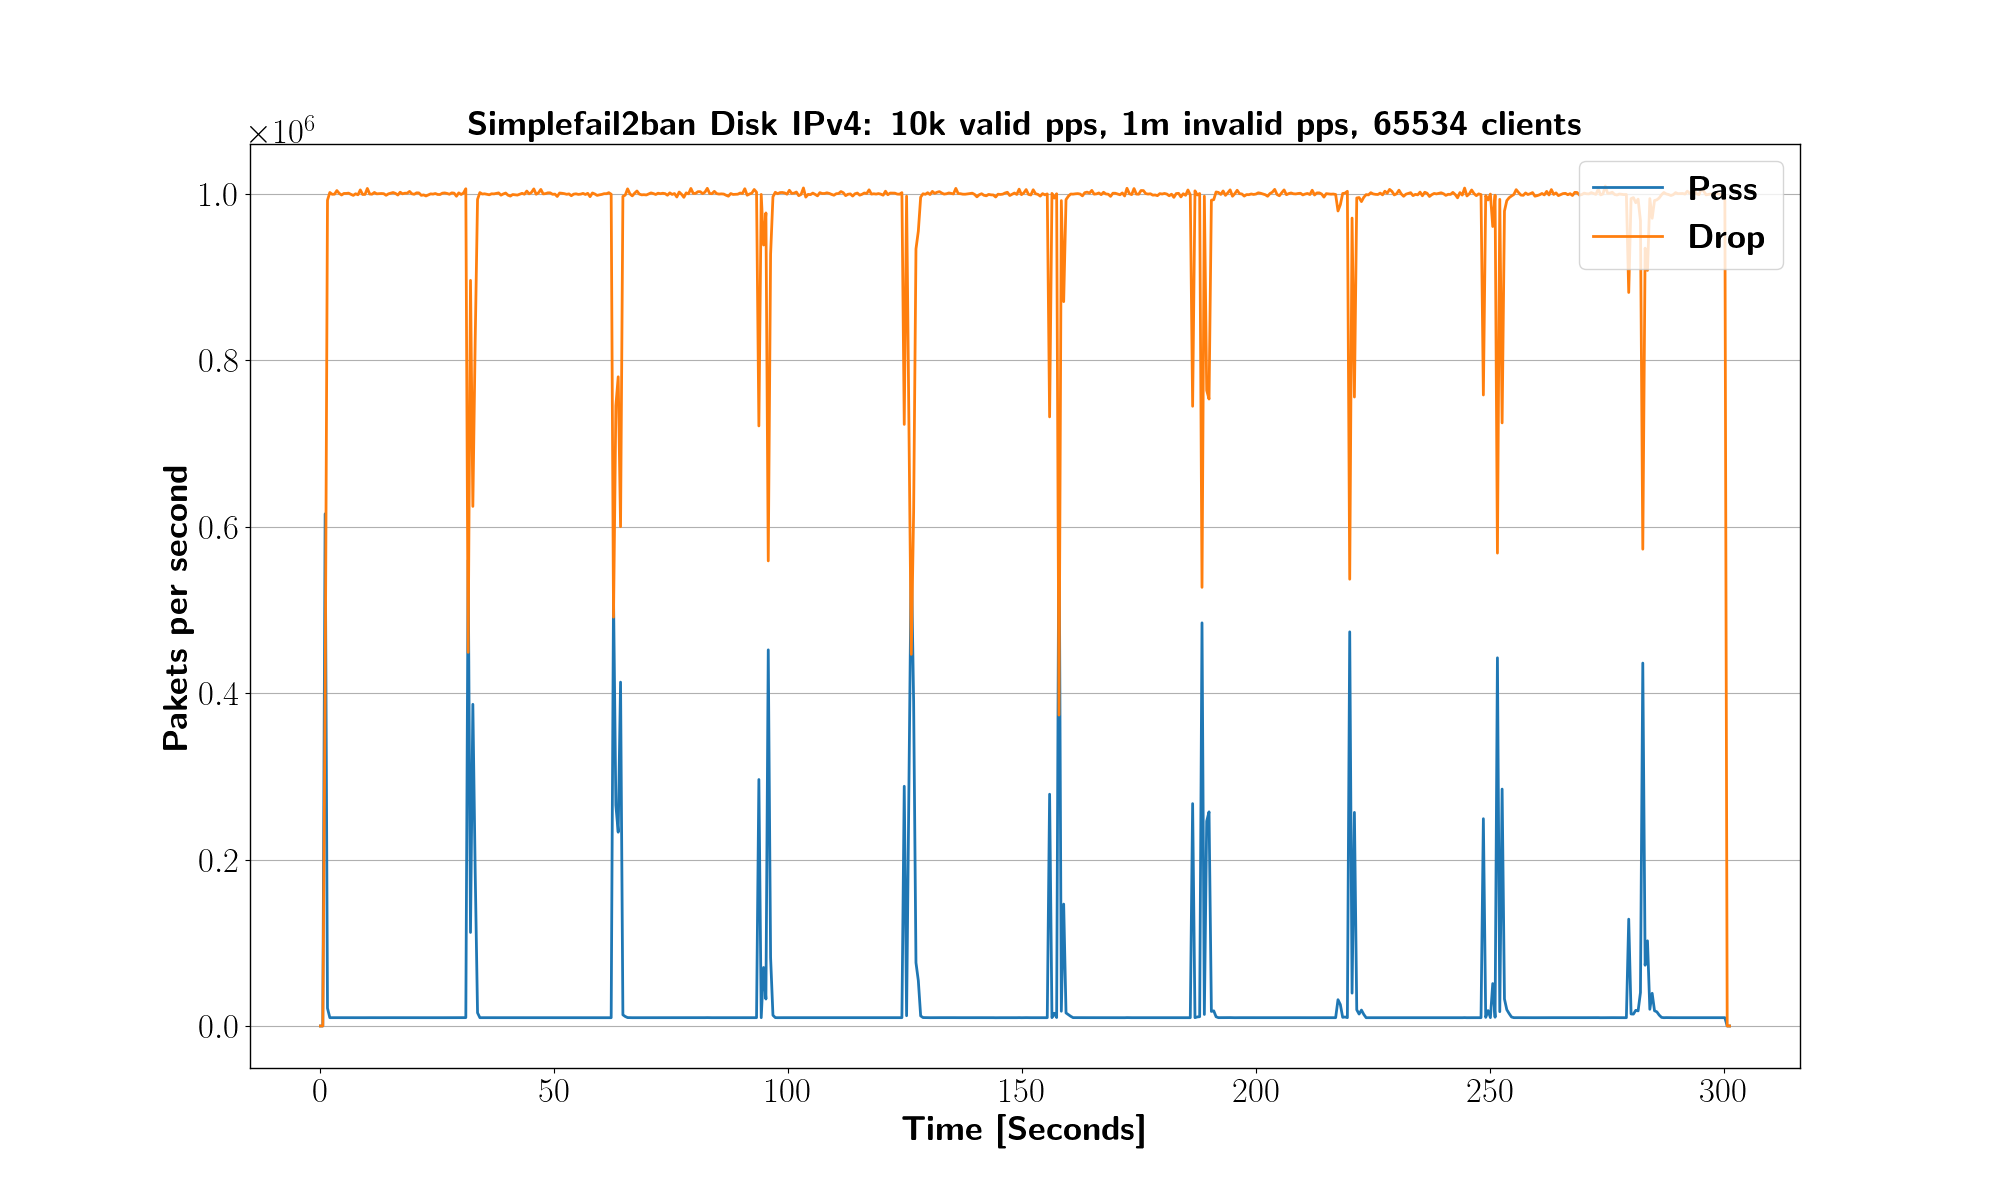
\includegraphics[width=1.2\textwidth]{images/simplefail2ban_disk_ipv4_v10k_iv1m_c65534.png}}
    \end{tabular}
	\begin{tabular}{lllll}
		\toprule
		\textbf{Total packets [$10^6$]} & \textbf{Packets dropped [$10^6$]} & \textbf{Relative drop [\%]} & \textbf{Log messages [$10^6$]} & \textbf{CPU [seconds]} \\ \midrule 
		303 & 294.43 & 98.79 & 4.7 & 14.99 \\
		\bottomrule
	\end{tabular}
	\caption[Simplefail2ban, Logfile IPv4, 1m \ac{PPS}]{Simplefail2ban Logfile \ac{IPv4}, 10 thousand unwanted \ac{PPS}, 1 million wanted \ac{PPS}, 65534 clients.}
	\label{fig:simplefail2ban:disk:ip4:1m}
\end{figure}

\begin{figure}[h!]
	\centering
	\scriptsize
	\begin{tabular}{c}
    	\centerline{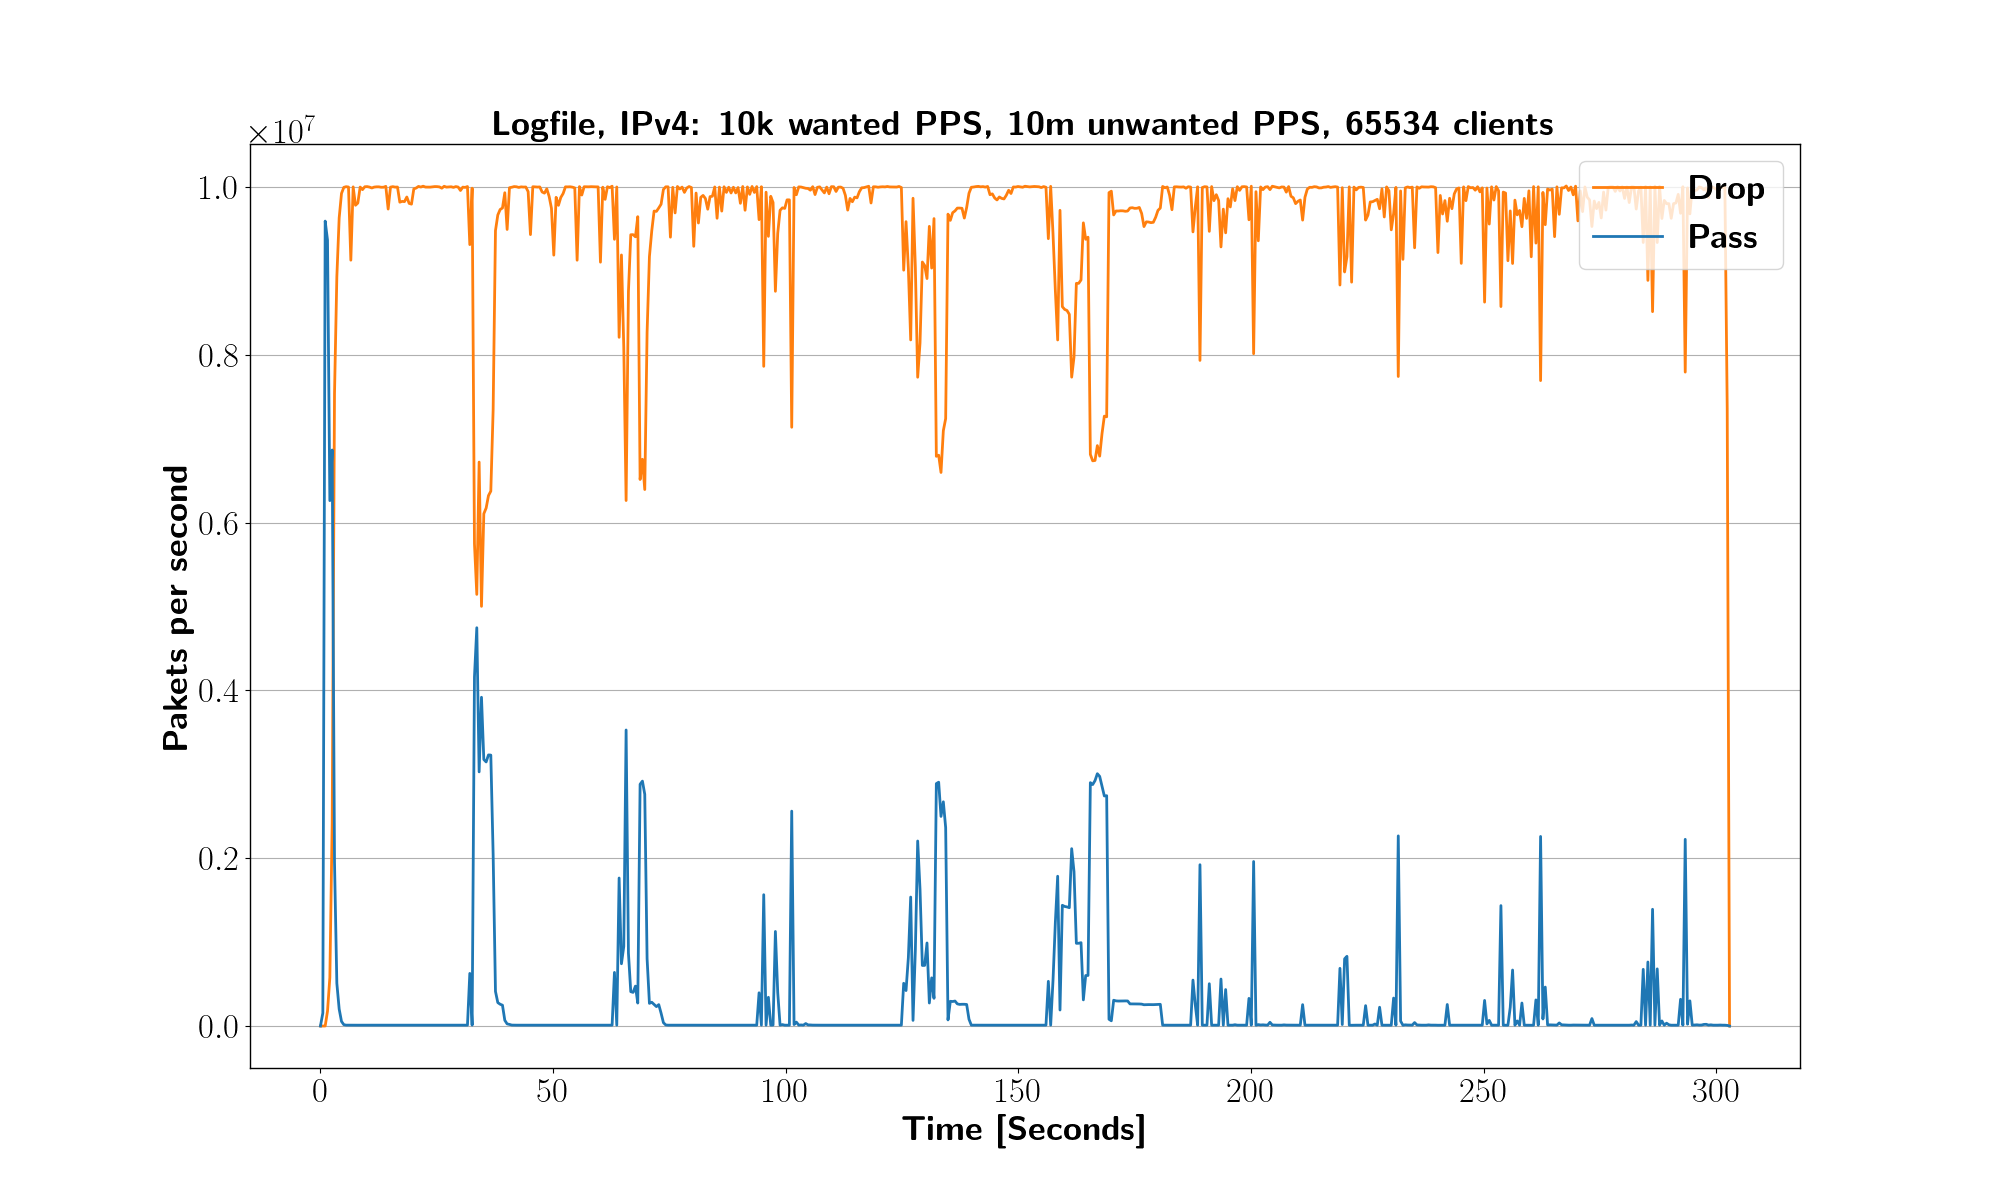
\includegraphics[width=1.2\textwidth]{images/simplefail2ban_disk_ipv4_v10k_iv10m_c65534.png}}
	\end{tabular}
	\begin{tabular}{lllll}
		\toprule
		\textbf{Total packets [$10^6$]} & \textbf{Packets dropped [$10^6$]} & \textbf{Relative drop [\%]} & \textbf{Log messages [$10^6$]} & \textbf{CPU [seconds]} \\ \midrule 
		2986.89 & 2884.14 & 96.72 & 34.39 & 83.72 \\
		\bottomrule
	\end{tabular}
	\caption[Simplefail2ban, Logfile IPv4, 10m \ac{PPS}]{Simplefail2ban Logfile \ac{IPv4}, 10 thousand unwanted \ac{PPS}, 10 million wanted \ac{PPS}, 65534 clients.}
	\label{fig:simplefail2ban:disk:ip4:10m}
\end{figure}

\begin{figure}[!h]
	\centering
	\scriptsize
	\begin{tabular}{c}
    	\centerline{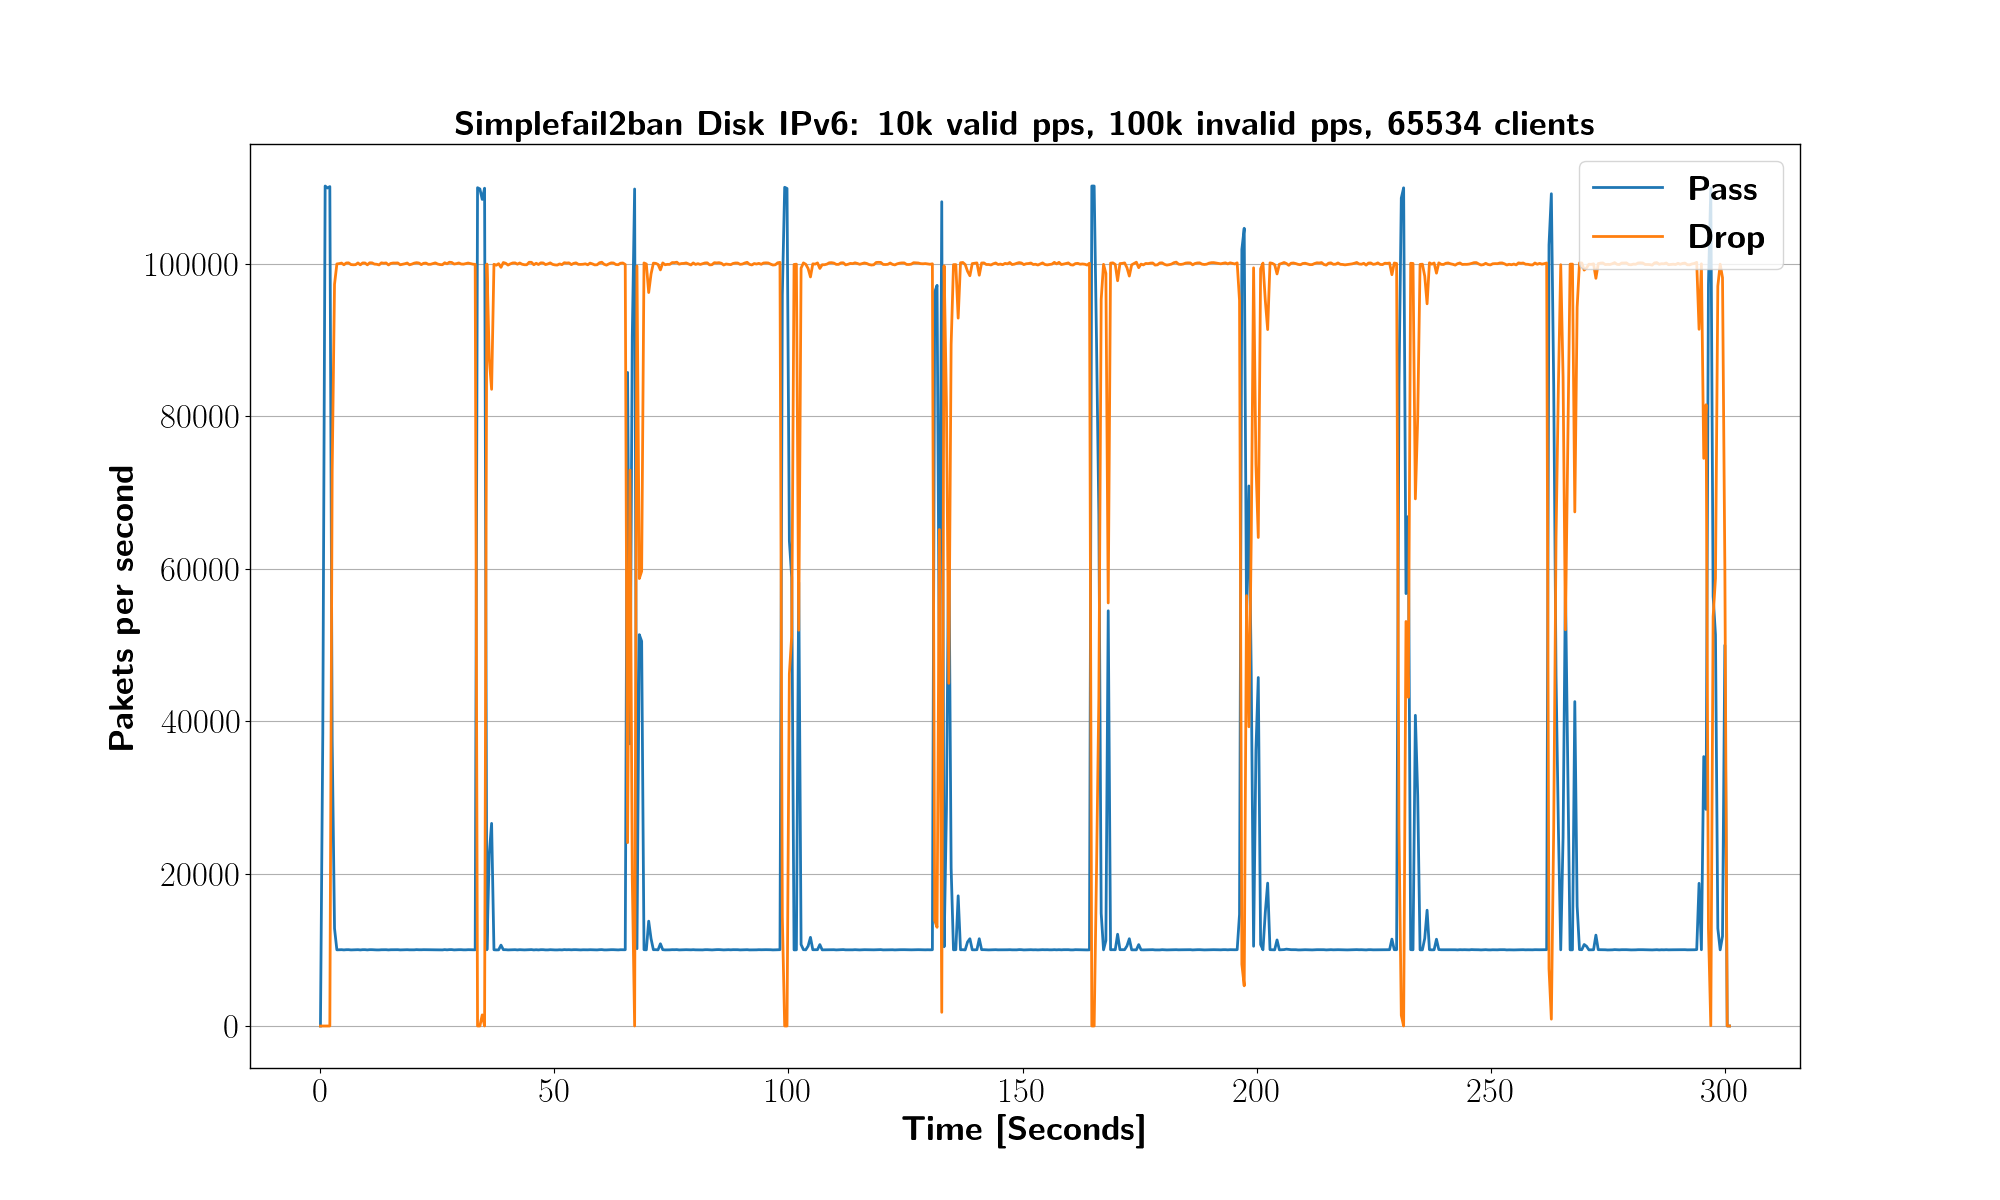
\includegraphics[width=1.2\textwidth]{images/simplefail2ban_disk_ipv6_v10k_iv100k_c65534.png}}
	\end{tabular}
	\begin{tabular}{lllll}
		\toprule
		\textbf{Total packets [$10^6$]} & \textbf{Packets dropped [$10^6$]} & \textbf{Relative drop [\%]} & \textbf{Log messages [$10^6$]} & \textbf{CPU [seconds]} \\ \midrule 
		33 & 27.96 & 99.67 & 2.04 & 11.75 \\
		\bottomrule
	\end{tabular}
	\caption[Simplefail2ban, Logfile IPv6, 100k \ac{PPS}]{Simplefail2ban Logfile \ac{IPv6}, 10 thousand wanted \ac{PPS}, 100 thousand unwanted \ac{PPS}, 65534 clients.}
	\label{fig:simplefail2ban:disk:ip6:100k}
\end{figure}

\begin{figure}[!h]
	\centering
	\scriptsize
	\begin{tabular}{c}
    	\centerline{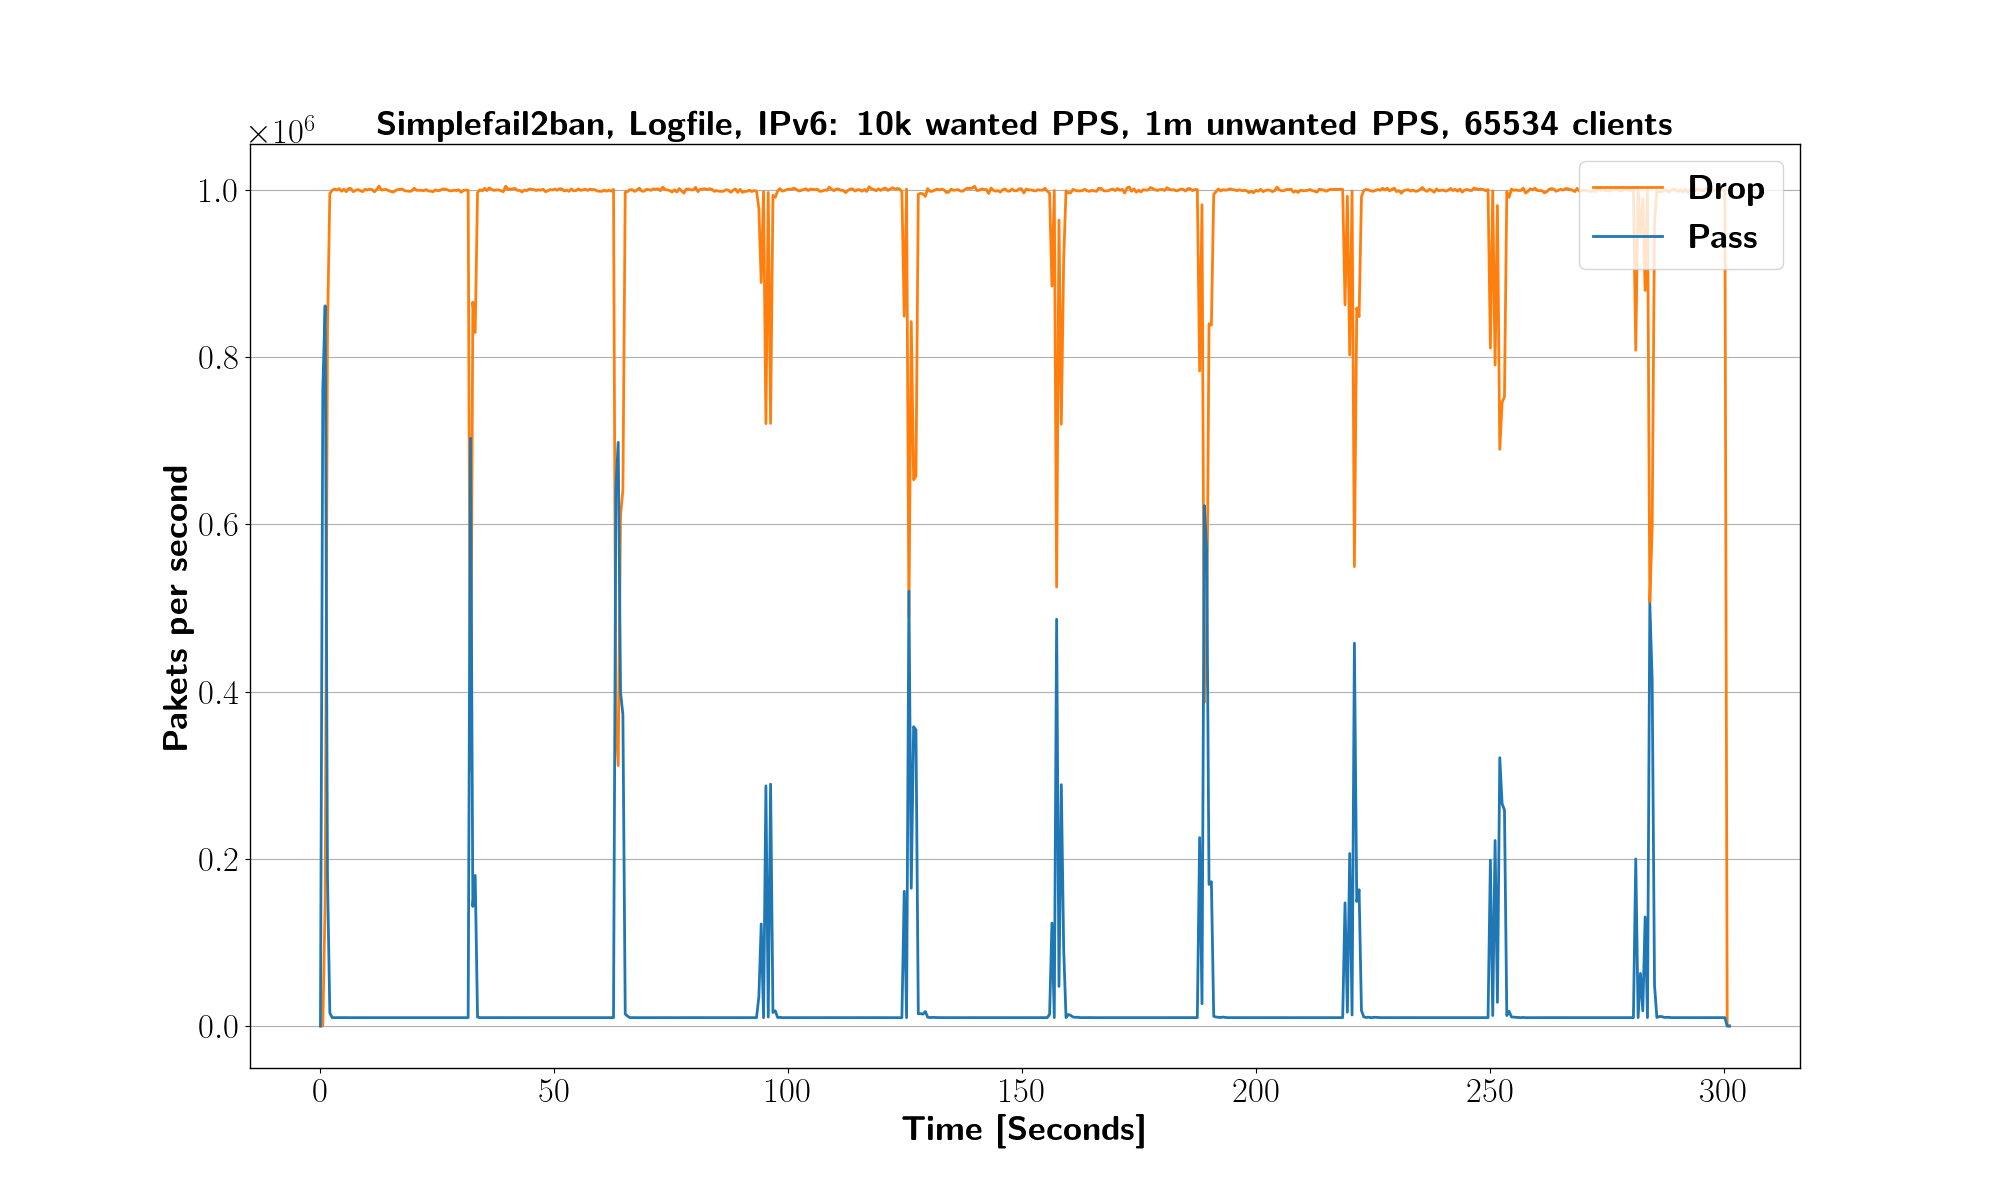
\includegraphics[width=1.2\textwidth]{images/simplefail2ban_disk_ipv6_v10k_iv1m_c65534.png}}
	\end{tabular}
	\begin{tabular}{lllll}
		\toprule
		\textbf{Total packets [$10^6$]} & \textbf{Packets dropped [$10^6$]} & \textbf{Relative drop [\%]} & \textbf{Log messages [$10^6$]} & \textbf{CPU [seconds]} \\ \midrule 
		303 & 293.49 & 98.48 & 5.58 & 21.08 \\
		\bottomrule
	\end{tabular}
	\caption[Simplefail2ban, Logfile IPv6, 1m \ac{PPS}]{Simplefail2ban Logfile \ac{IPv6}, 10 thousand wanted \ac{PPS}, 1 million unwanted \ac{PPS}, 65534 clients.}
	\label{fig:simplefail2ban:disk:ip6:1m}
\end{figure}

\begin{figure}[!h]
	\centering
	\scriptsize
	\begin{tabular}{c}
    	\centerline{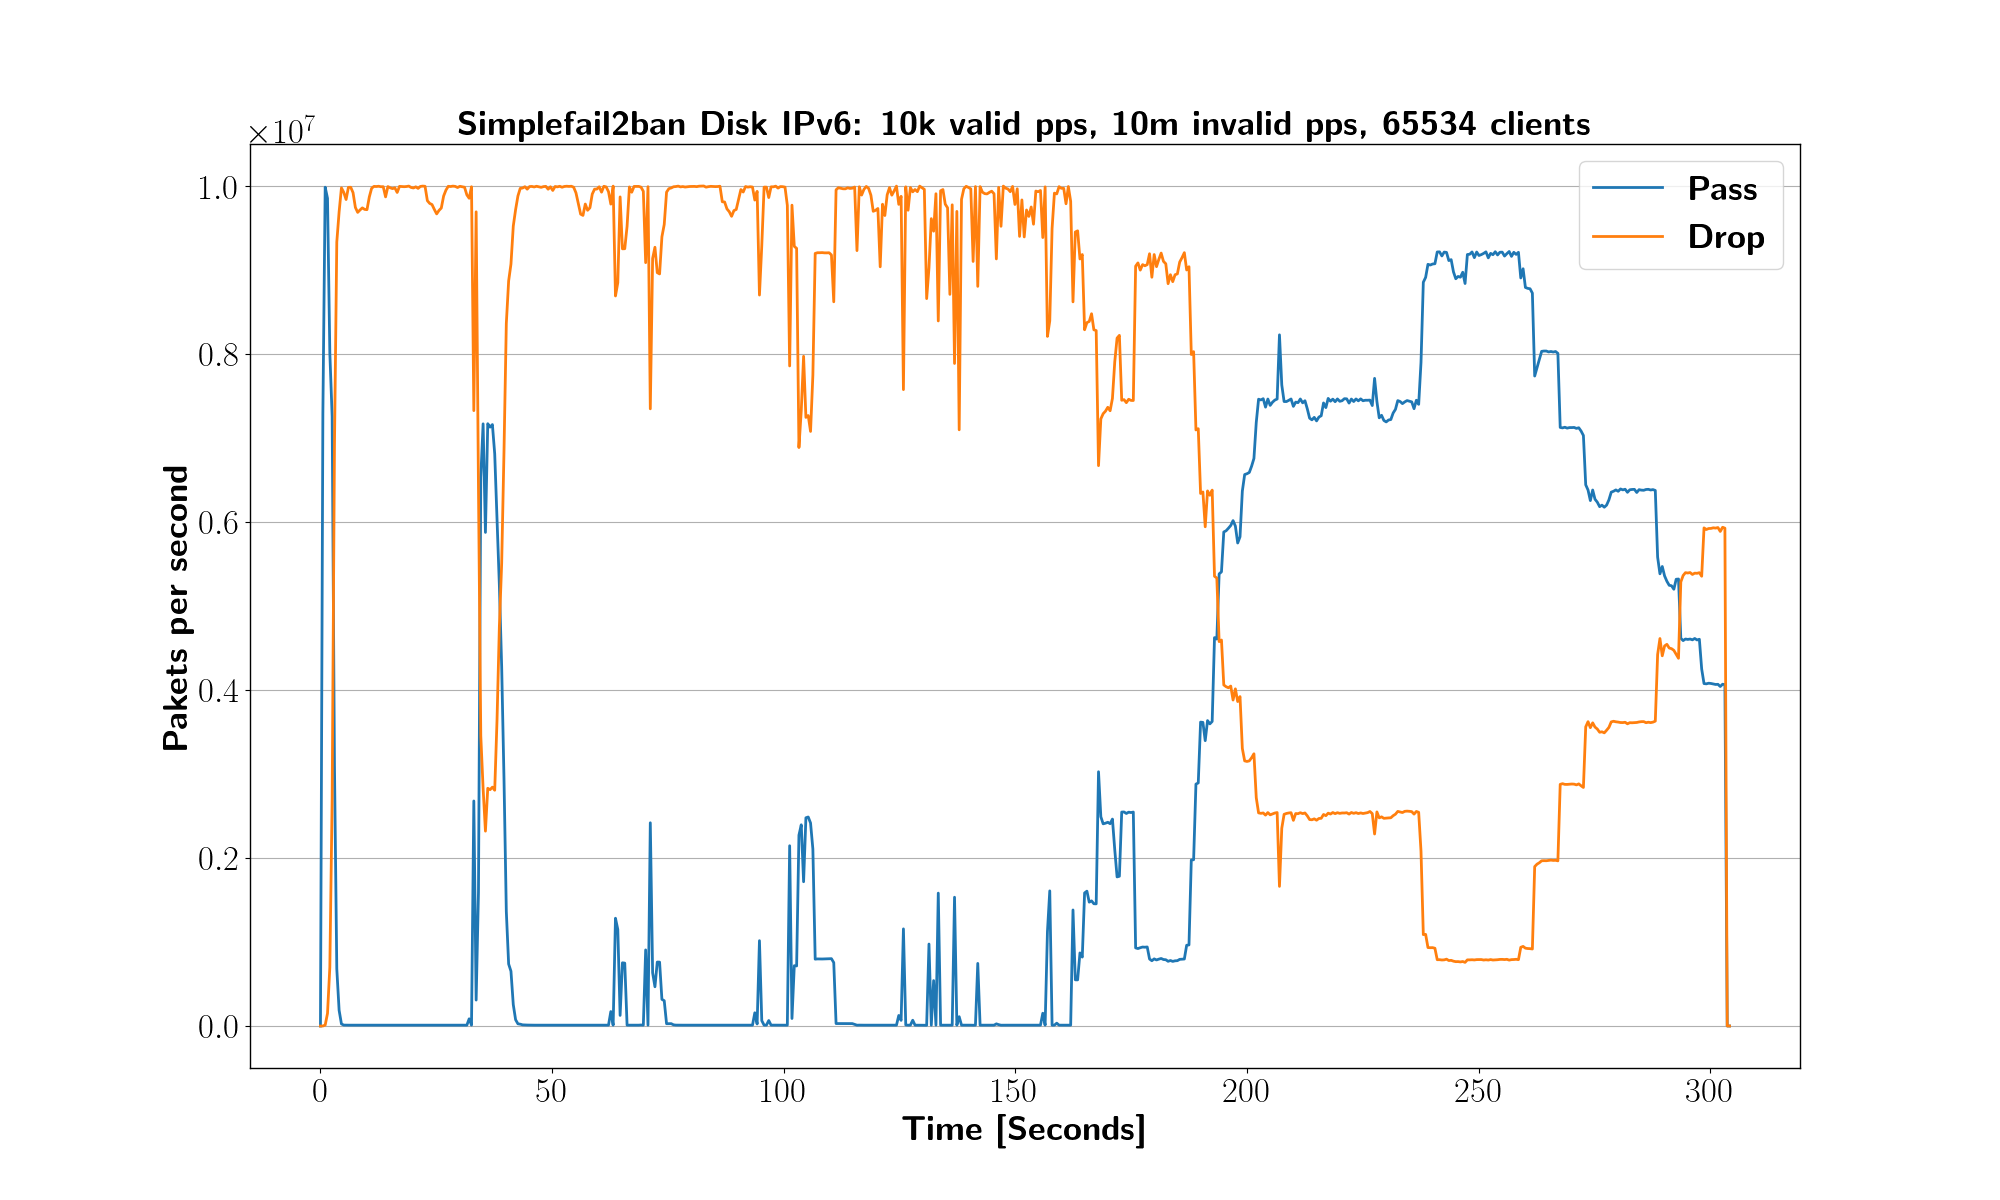
\includegraphics[width=1.2\textwidth]{images/simplefail2ban_disk_ipv6_v10k_iv10m_c65534.png}}
	\end{tabular}
	\begin{tabular}{lllll}
		\toprule
		\textbf{Total packets [$10^6$]} & \textbf{Packets dropped [$10^6$]} & \textbf{Relative drop [\%]} & \textbf{Log messages [$10^6$]} & \textbf{CPU [seconds]} \\ \midrule 
		2992.43 & 2065.28 & 69.13 & 205.4 & 346.73 \\
		\bottomrule
	\end{tabular}
	\caption[Simplefail2ban, Logfile IPv6, 10m \ac{PPS}]{Simplefail2ban Logfile \ac{IPv6}, 10 thousand wanted \ac{PPS}, 10 million unwanted \ac{PPS}, 65534 clients.}
	\label{fig:simplefail2ban:disk:ip6:10m}
\end{figure}


\begin{figure}[!h]
	\centering
	\scriptsize
	\begin{tabular}{c}
    	\centerline{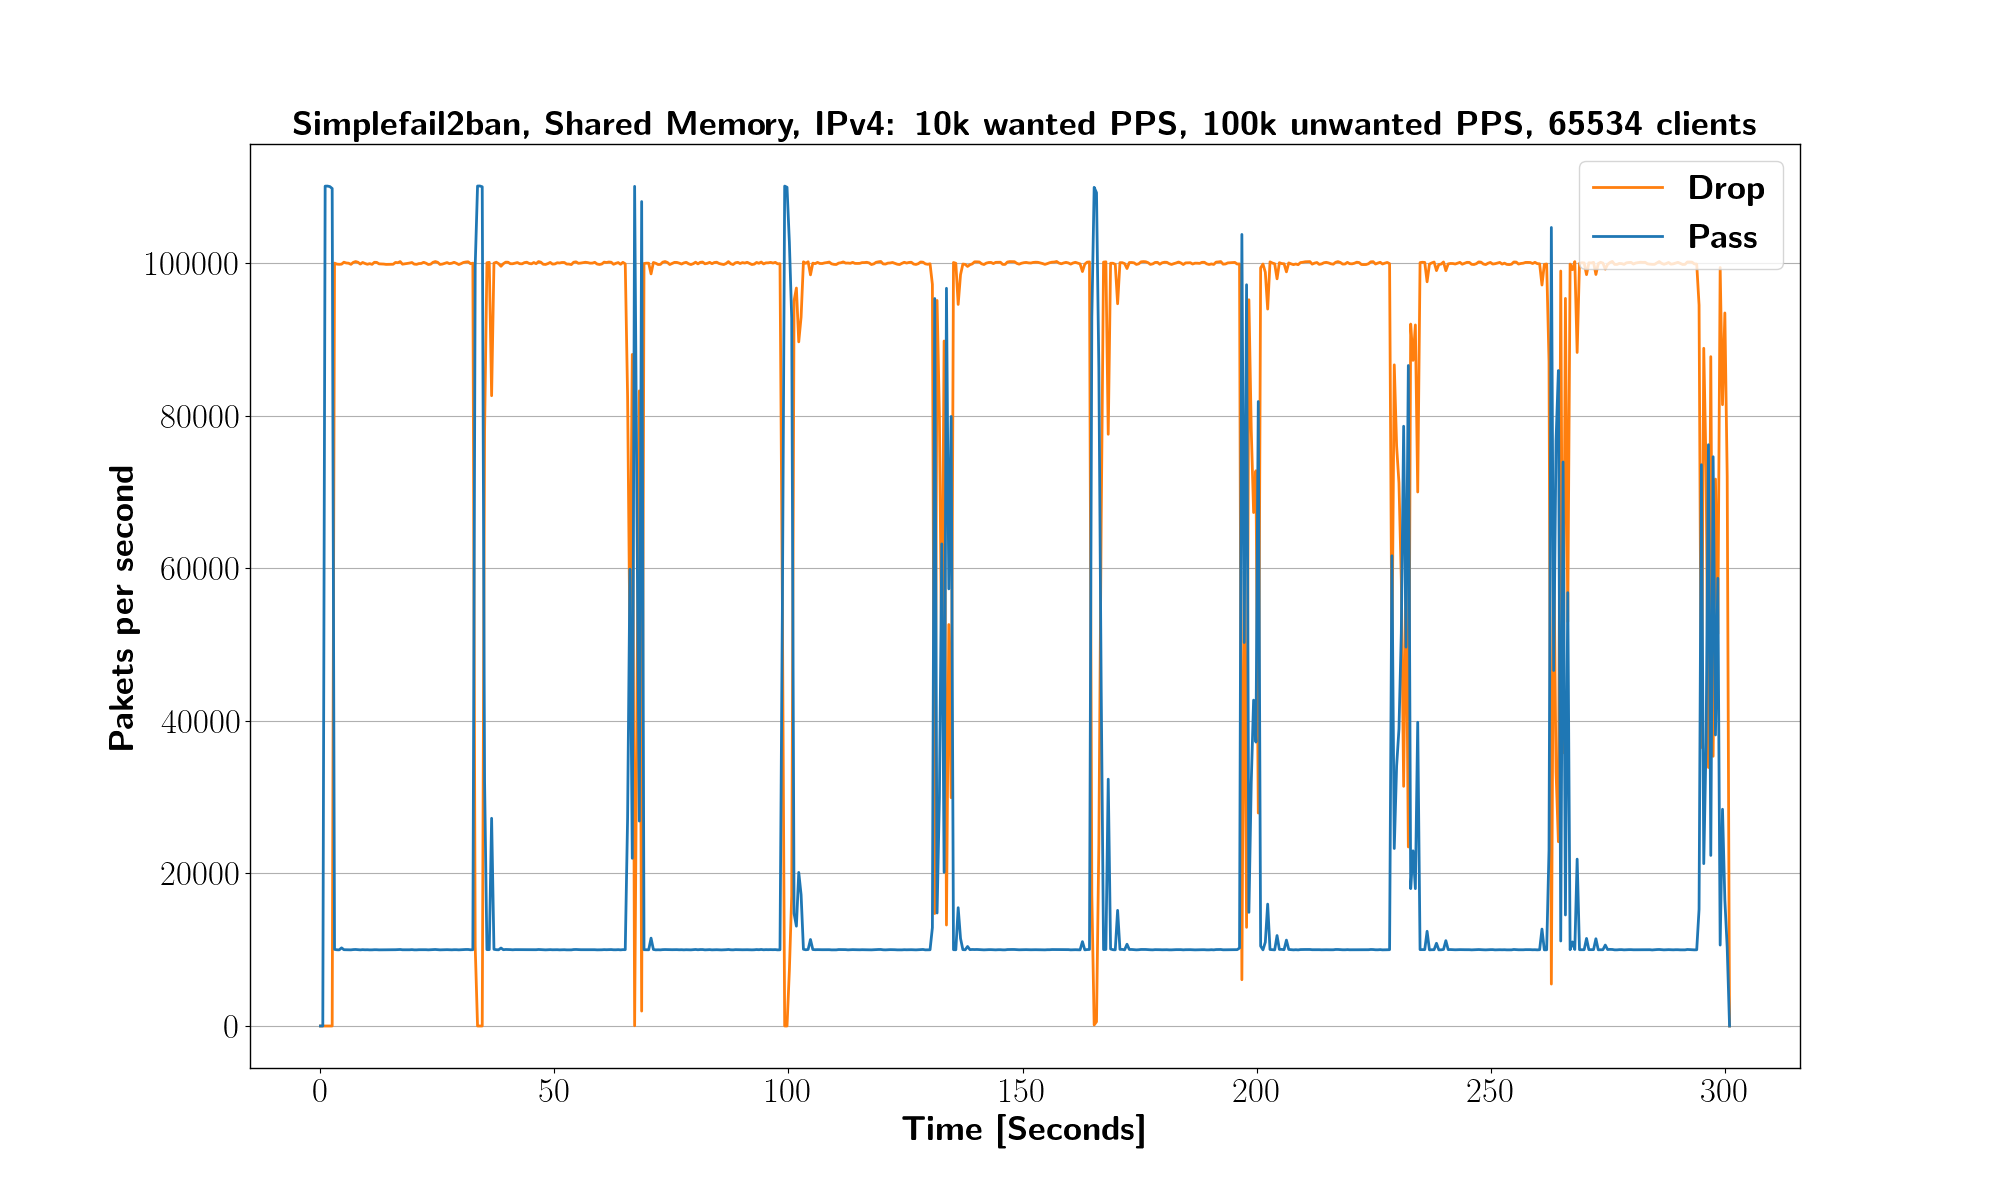
\includegraphics[width=1.2\textwidth]{images/simplefail2ban_shm_ipv4_v10k_iv100k_c65534.png}}
	\end{tabular}
	\begin{tabular}{lllll}
		\toprule
		\textbf{Total packets [$10^6$]} & \textbf{Packets dropped [$10^6$]} & \textbf{Relative drop [\%]} & \textbf{Log messages [$10^6$]} & \textbf{CPU [seconds]} \\ \midrule 
		33 & 27.95 & 99.64 & 2.05 & 13.68 \\
		\bottomrule
	\end{tabular}
	\caption[Simplefail2ban, Shared Memory, IPv4, 100k \ac{PPS}]{Simplefail2ban Shared Memory \ac{IPv4}, 10 thousand wanted \ac{PPS}, 100 thousand unwanted \ac{PPS}, 65534 clients.}
	\label{fig:simplefail2ban:shm:ip4:100k}
\end{figure}

\begin{figure}[!h]
	\centering
	\scriptsize
	\begin{tabular}{c}
    	\centerline{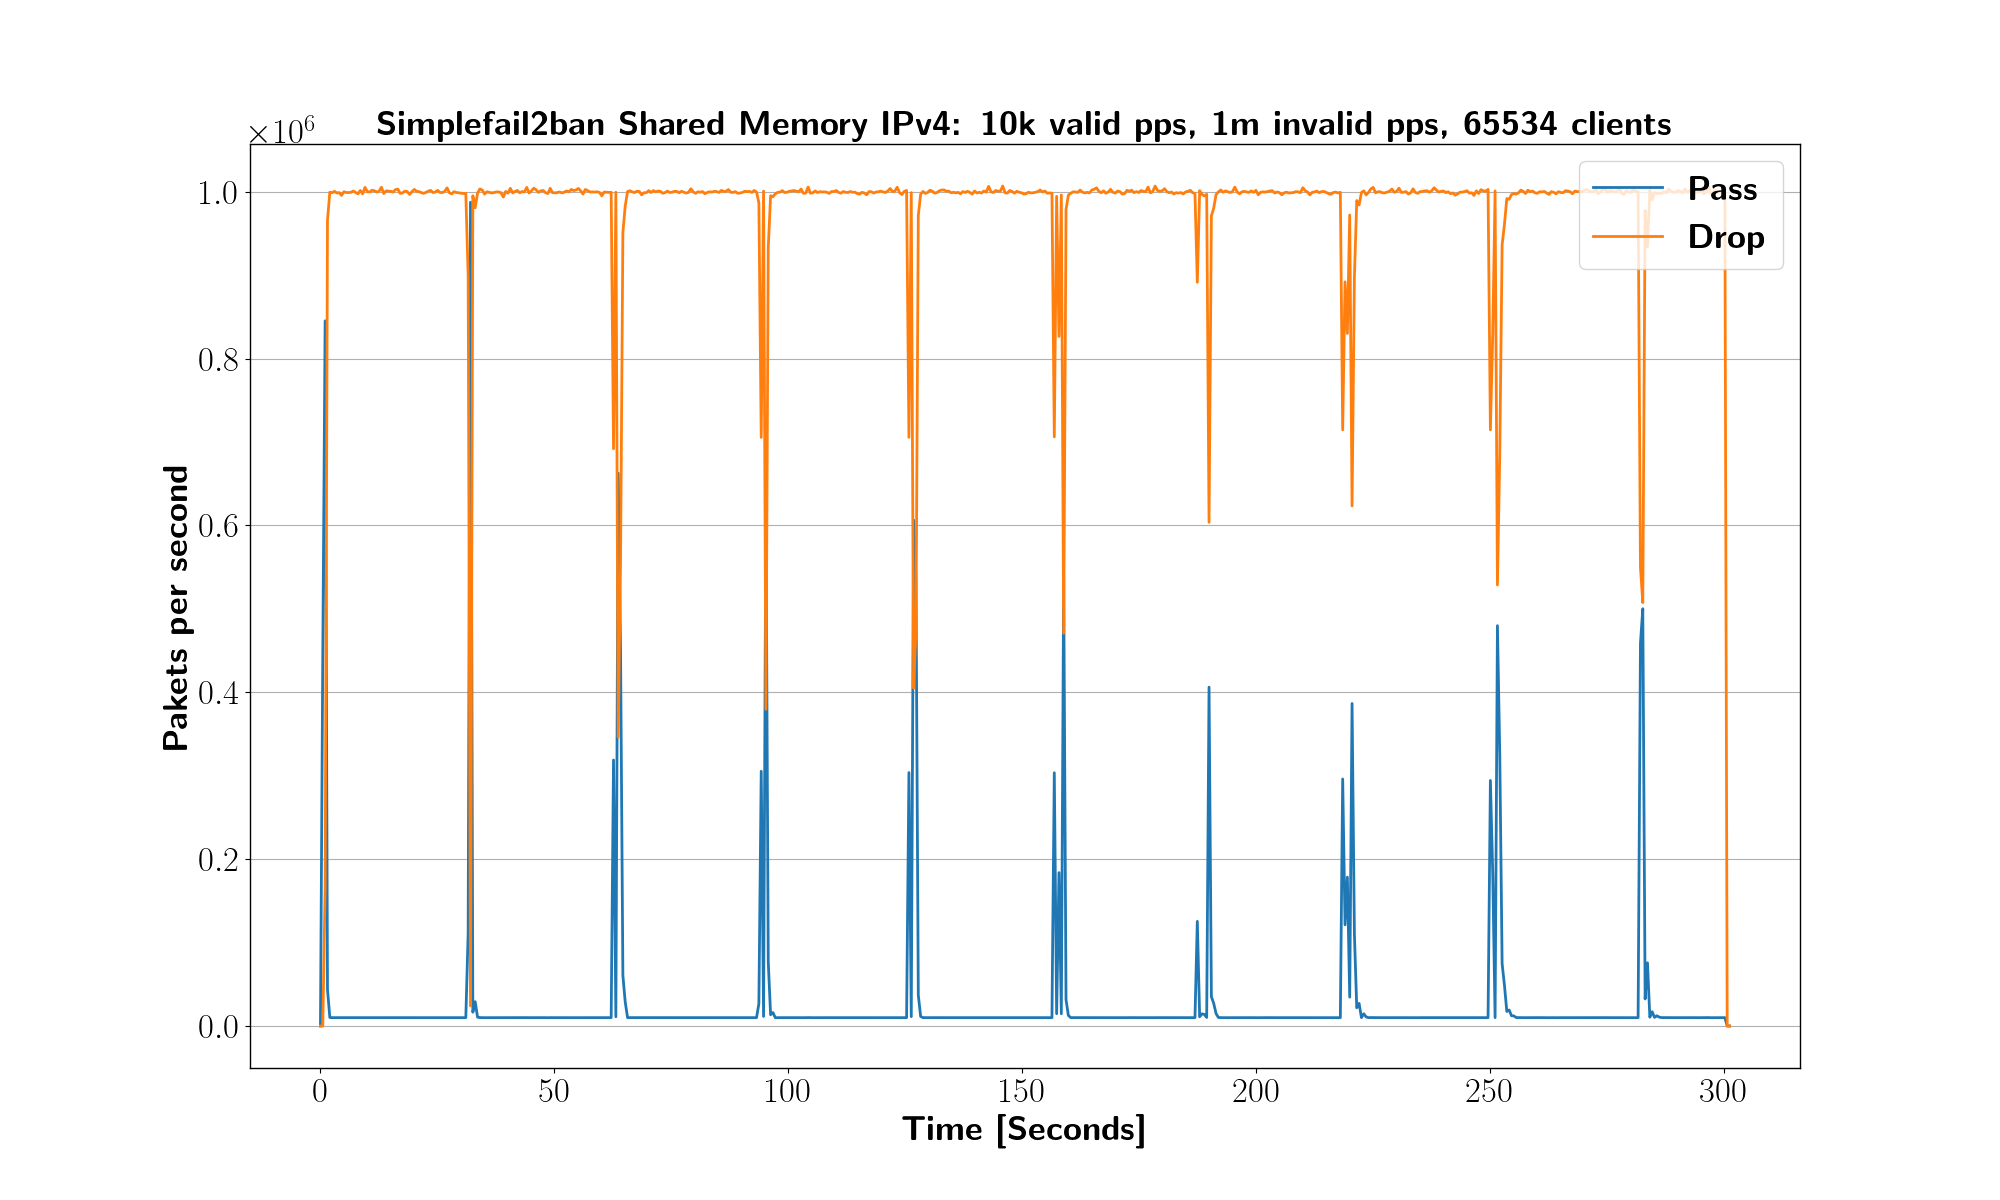
\includegraphics[width=1.2\textwidth]{images/simplefail2ban_shm_ipv4_v10k_iv1m_c65534.png}}
	\end{tabular}
	\begin{tabular}{lllll}
		\toprule
		\textbf{Total packets [$10^6$]} & \textbf{Packets dropped [$10^6$]} & \textbf{Relative drop [\%]} & \textbf{Log messages [$10^6$]} & \textbf{CPU [seconds]} \\ \midrule 
		303 & 294.34 & 98.88 & 4.61 & 15.52 \\
		\bottomrule
	\end{tabular}
	\caption[Simplefail2ban, Shared Memory, IPv4, 1m \ac{PPS}]{Simplefail2ban Shared Memory \ac{IPv4}, 10 thousand wanted \ac{PPS}, 10 million unwanted \ac{PPS}, 65534 clients.}
	\label{fig:simplefail2ban:shm:ip4:1m}
\end{figure}

\begin{figure}[!h]
	\centering
	\scriptsize
	\begin{tabular}{c}
    	\centerline{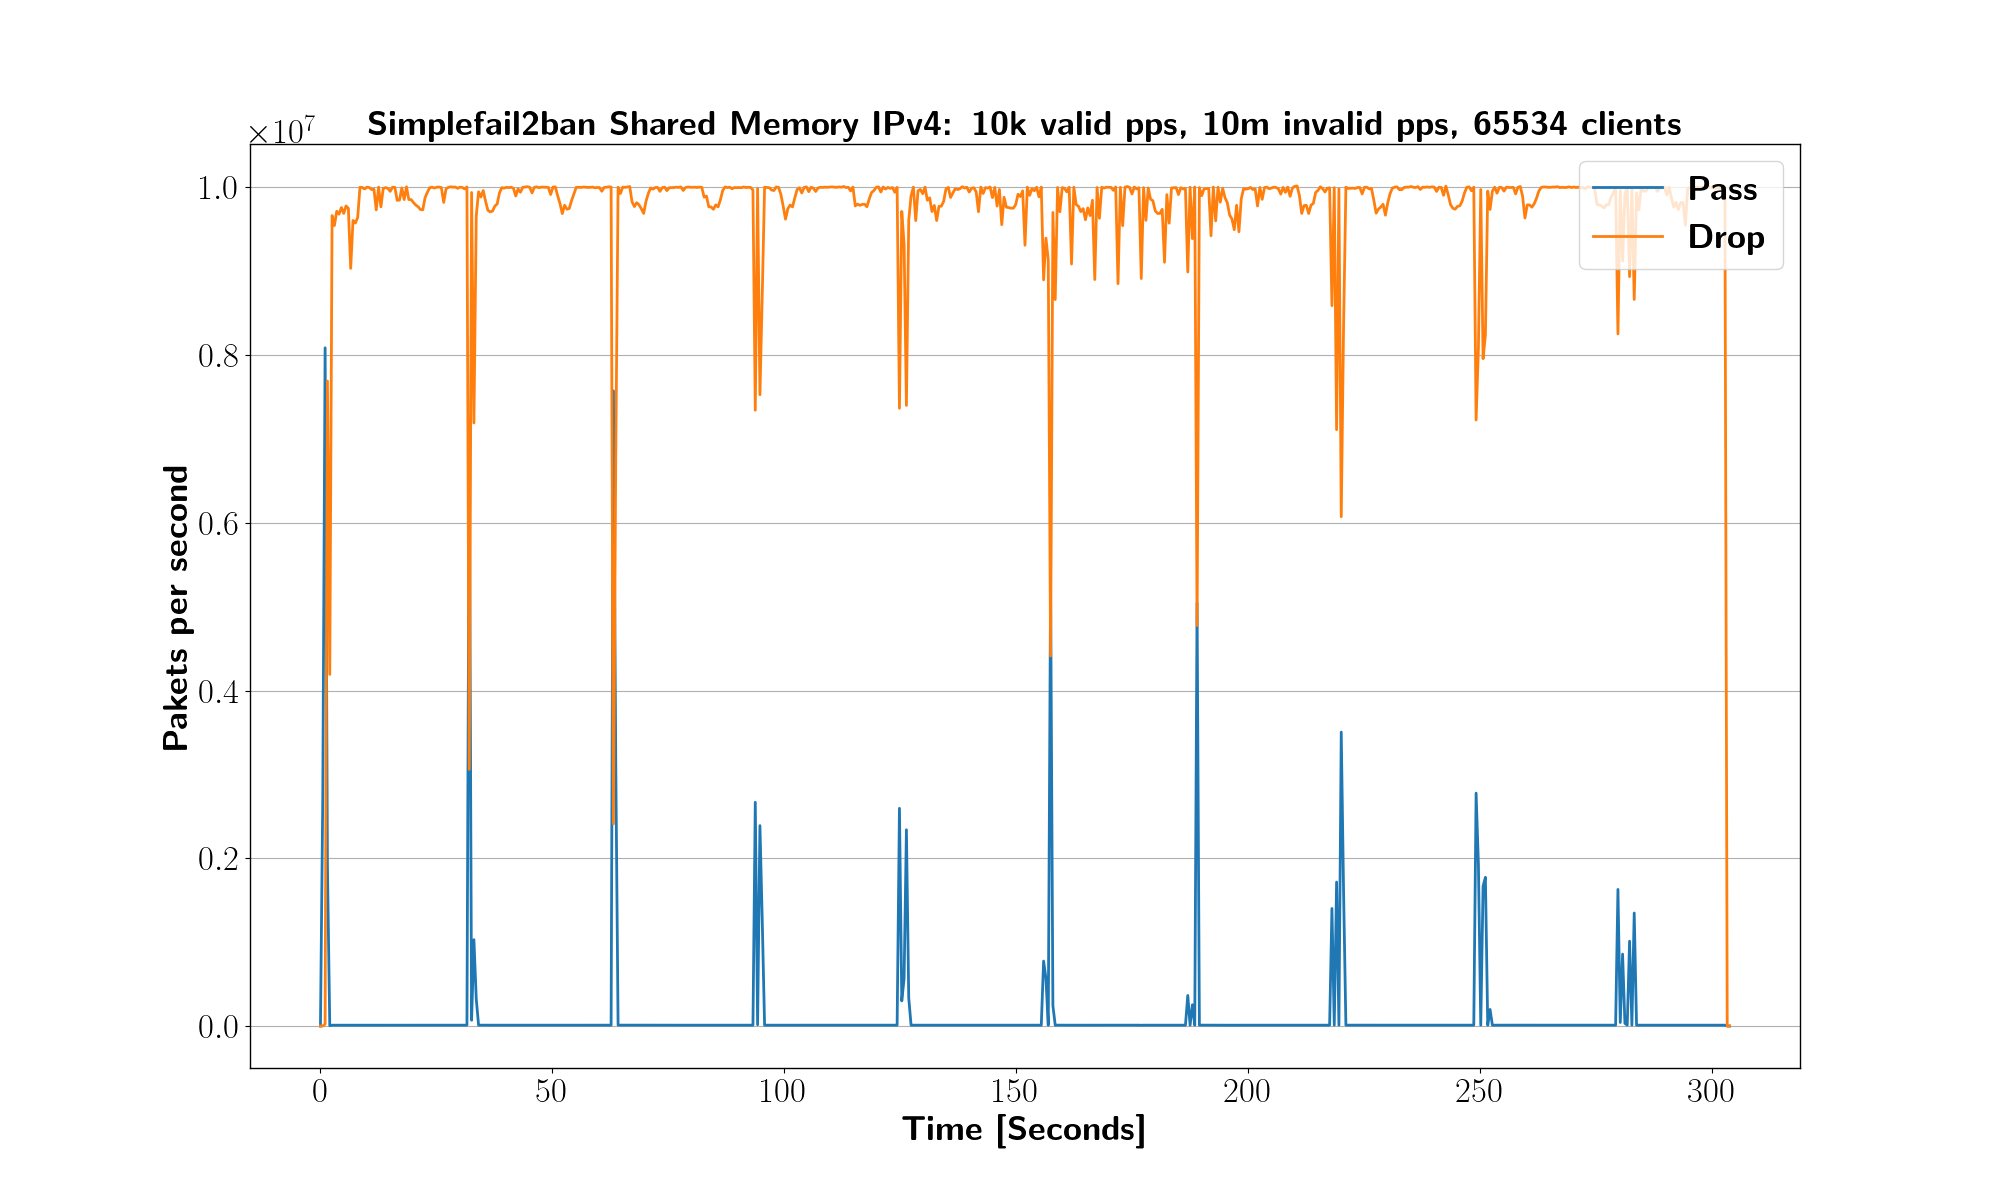
\includegraphics[width=1.2\textwidth]{images/simplefail2ban_shm_ipv4_v10k_iv10m_c65534.png}}
	\end{tabular}
	\begin{tabular}{lllll}
		\toprule
		\textbf{Total packets [$10^6$]} & \textbf{Packets dropped [$10^6$]} & \textbf{Relative drop [\%]} & \textbf{Log messages [$10^6$]} & \textbf{CPU [seconds]} \\ \midrule 
		2991.48 & 2948.51 & 96.72 & 7.69 & 25.59 \\
		\bottomrule
	\end{tabular}
	\caption[Simplefail2ban, Shared Memory, IPv4, 10m \ac{PPS}]{Simplefail2ban Shared Memory \ac{IPv4}, 10 thousand wanted \ac{PPS}, 10 million unwanted \ac{PPS}, 65534 clients.}
	\label{fig:simplefail2ban:shm:ip4:10m}
\end{figure}

\begin{figure}[!h]
	\centering
	\scriptsize
	\begin{tabular}{c}
    	\centerline{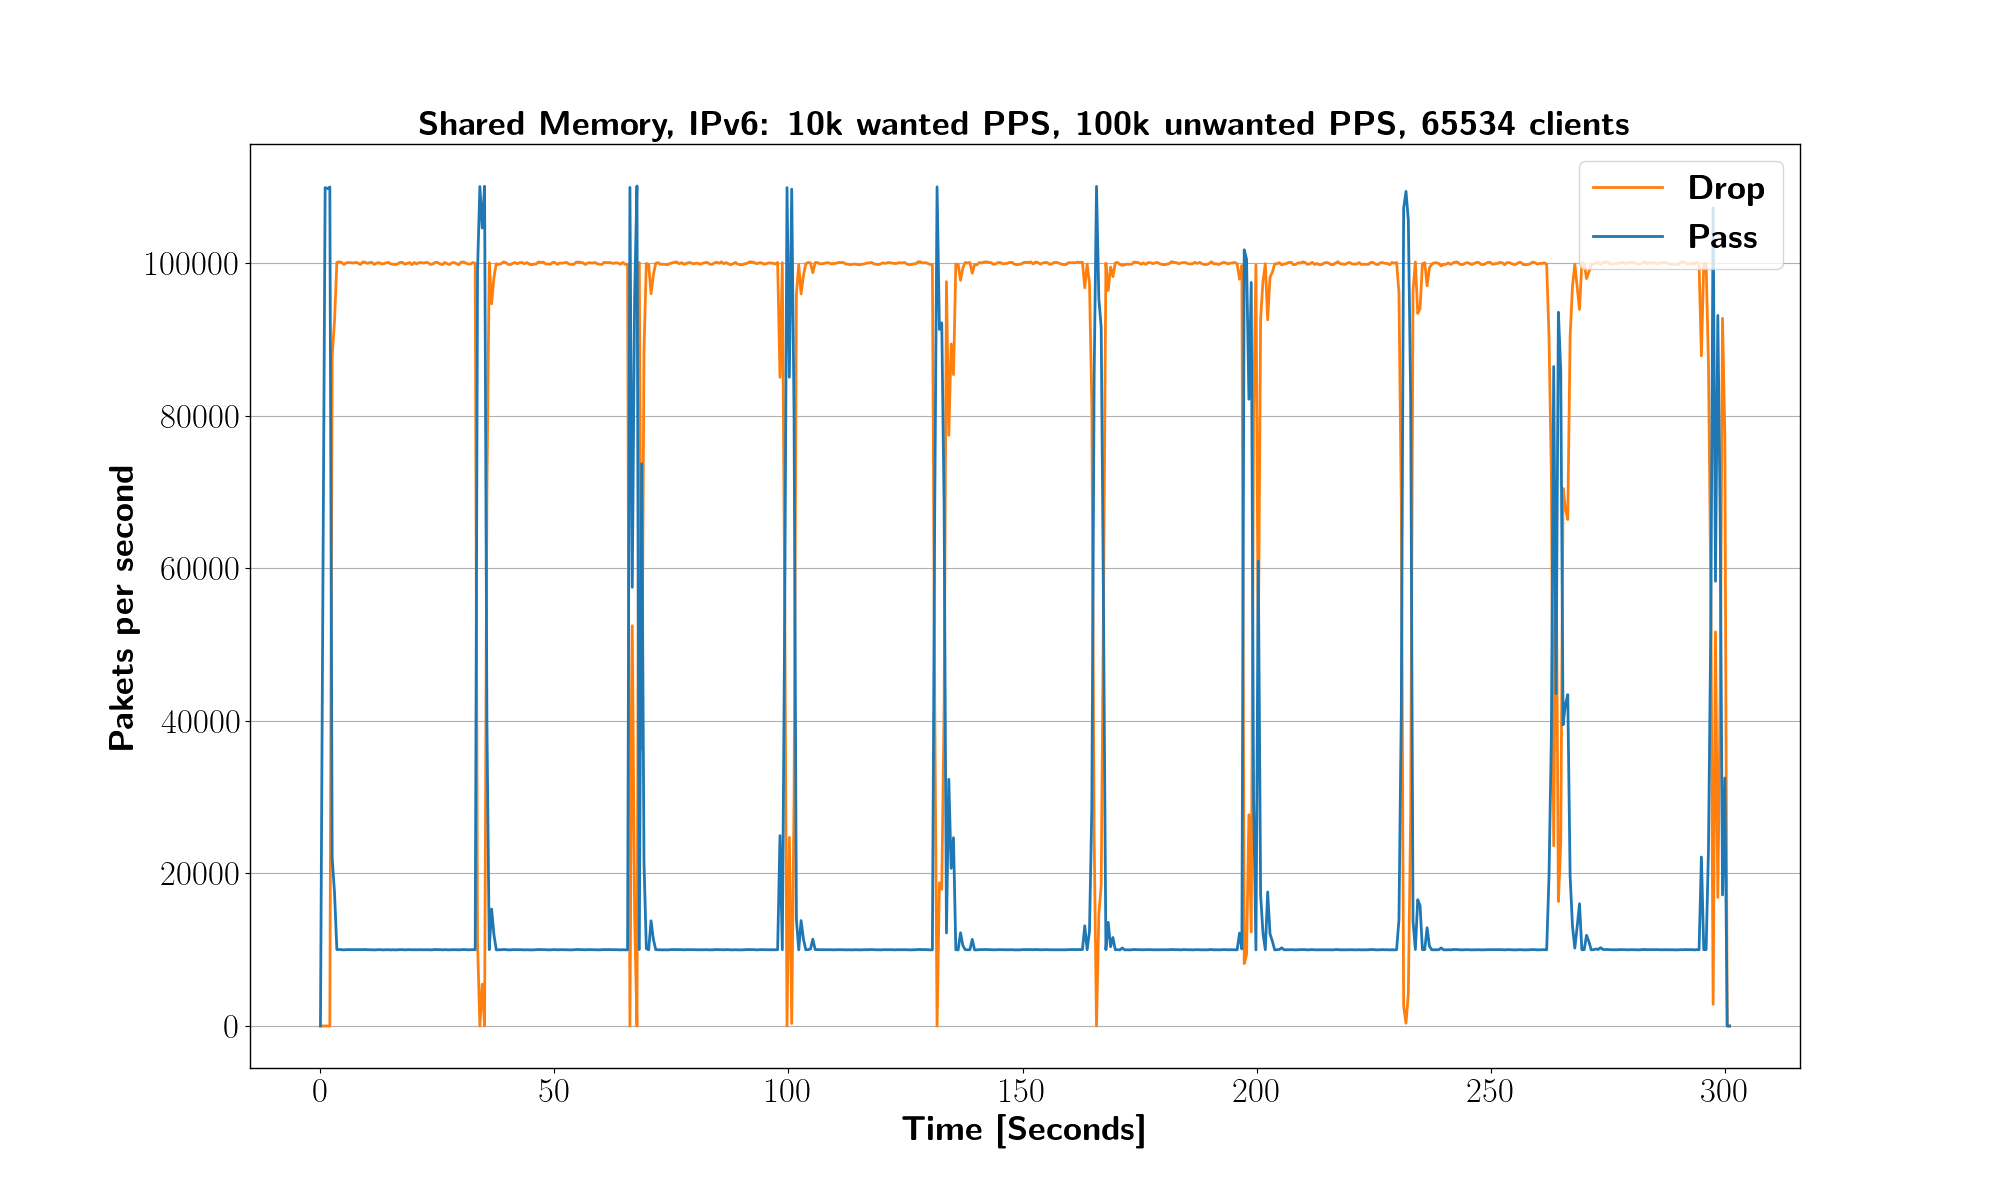
\includegraphics[width=1.2\textwidth]{images/simplefail2ban_shm_ipv6_v10k_iv100k_c65534.png}}
	\end{tabular}
	\begin{tabular}{lllll}
		\toprule
		\textbf{Total packets [$10^6$]} & \textbf{Packets dropped [$10^6$]} & \textbf{Relative drop [\%]} & \textbf{Log messages [$10^6$]} & \textbf{CPU [seconds]} \\ \midrule 
		33 & 27.95 & 99.67 & 2.05 & 15.55 \\
		\bottomrule
	\end{tabular}
	\caption[Simplefail2ban, Shared Memory, IPv6, 100k \ac{PPS}]{Simplefail2ban Shared Memory \ac{IPv6}, 10 thousand wanted \ac{PPS}, 100 thousand unwanted \ac{PPS}, 65534 clients.}
	\label{fig:simplefail2ban:shm:ip6:100k}
\end{figure}

\begin{figure}[!h]
	\centering
	\scriptsize
	\begin{tabular}{c}
    	\centerline{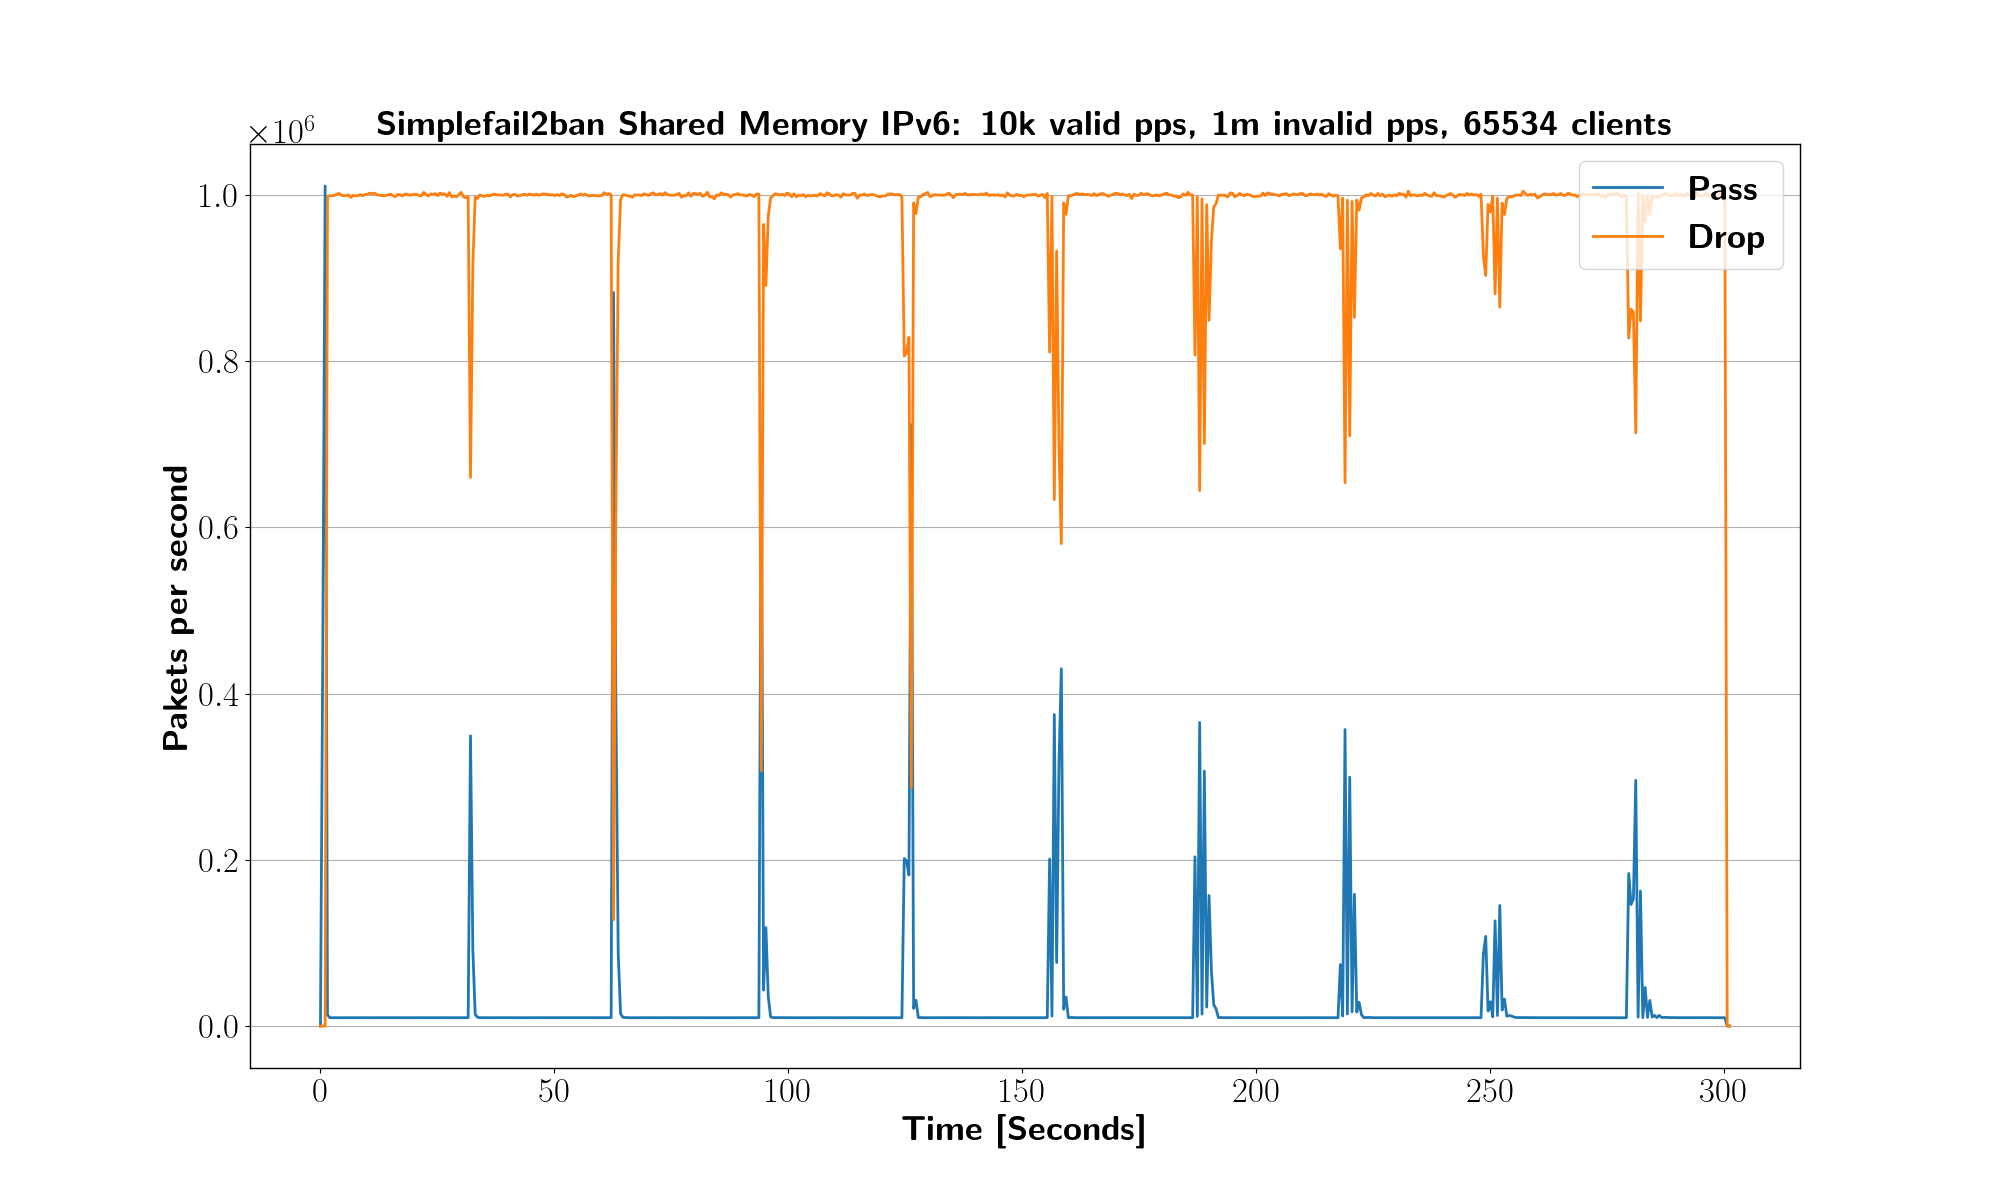
\includegraphics[width=1.2\textwidth]{images/simplefail2ban_shm_ipv6_v10k_iv1m_c65534.png}}
	\end{tabular}
	\begin{tabular}{lllll}
		\toprule
		\textbf{Total packets [$10^6$]} & \textbf{Packets dropped [$10^6$]} & \textbf{Relative drop [\%]} & \textbf{Log messages [$10^6$]} & \textbf{CPU [seconds]} \\ \midrule 
		303 & 294.77 & 98.9 & 4.39 & 17.46 \\
		\bottomrule
	\end{tabular}
	\caption[Simplefail2ban, Shared Memory, IPv6, 1m \ac{PPS}]{Simplefail2ban Shared Memory \ac{IPv6}, 10 thousand wanted \ac{PPS}, 1 million unwanted \ac{PPS}, 65534 clients.}
	\label{fig:simplefail2ban:shm:ip6:1m}
\end{figure}

\begin{figure}[!h]
	\centering
	\scriptsize
	\begin{tabular}{c}
    	\centerline{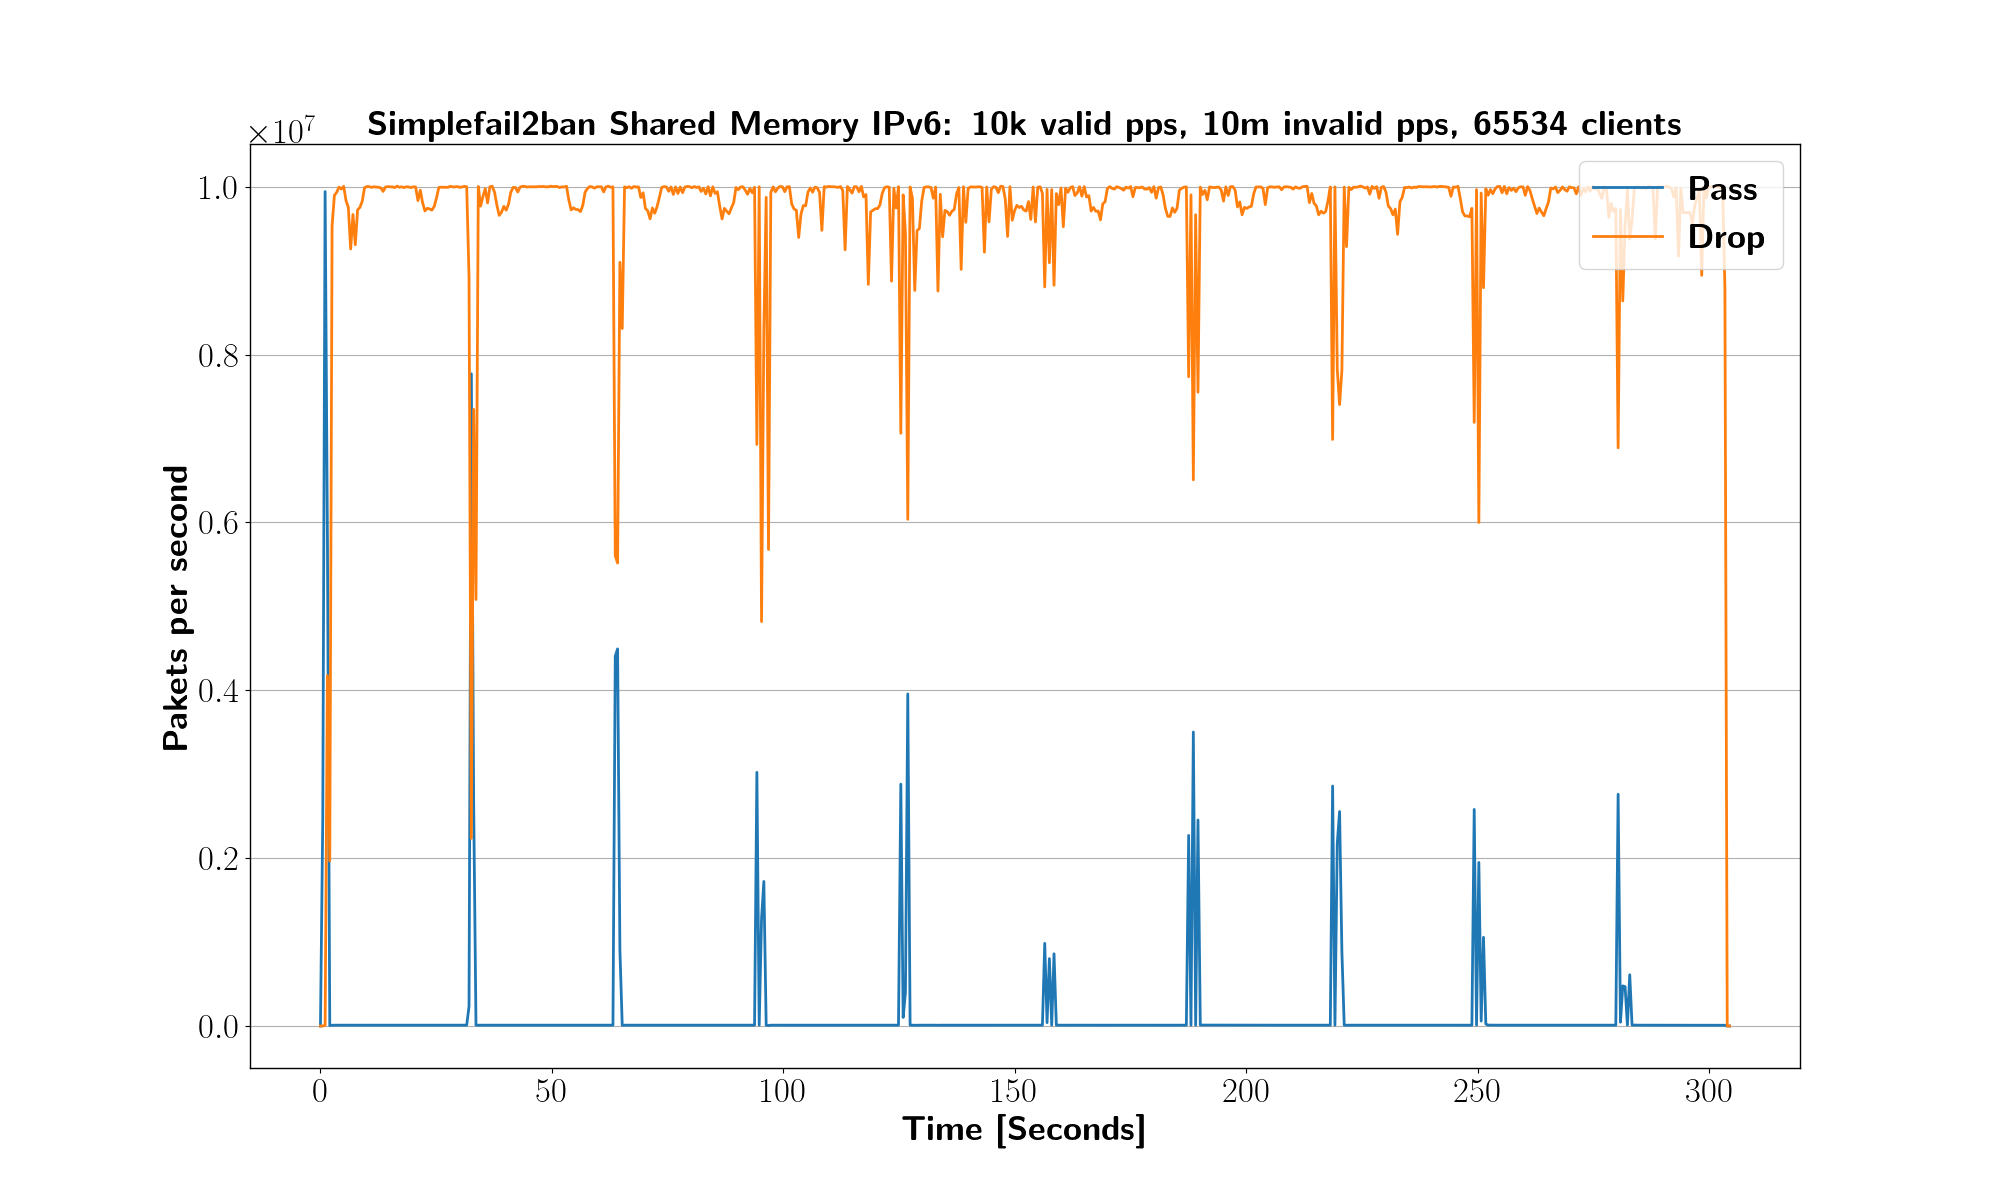
\includegraphics[width=1.2\textwidth]{images/simplefail2ban_shm_ipv6_v10k_iv10m_c65534.png}}
	\end{tabular}
	\begin{tabular}{lllll}
		\toprule
		\textbf{Total packets [$10^6$]} & \textbf{Packets dropped [$10^6$]} & \textbf{Relative drop [\%]} & \textbf{Log messages [$10^6$]} & \textbf{CPU [seconds]} \\ \midrule 
		2991.93 & 2947.1 & 98.66 & 8.88 & 32.36 \\
		\bottomrule
	\end{tabular}
	\caption[Simplefail2ban, Shared Memory, IPv6, 10m \ac{PPS}]{Simplefail2ban Shared Memory \ac{IPv6}, 10 thousand wanted \ac{PPS}, 10 million unwanted \ac{PPS}, 65534 clients.}
	\label{fig:simplefail2ban:shm:ip6:10m}
\end{figure}

%
% bibliography
%
\def\UrlBreaks{\do\/\do-}
% alphaurl is a special bibliography style which includes Hyperlinks 
% to papers
\begingroup
\sloppy
%\raggedright
\bibliographystyle{unsrt}
% bib file without extension
\bibliography{literature}
\endgroup


%\printindex 


\end{document}
